%----------------------------------------------------------------------------------------
%	PACKAGES AND OTHER DOCUMENT CONFIGURATIONS
%----------------------------------------------------------------------------------------
%\pdfmapline{-dummy RTTAOZ+CMMI10}
%\pdfmapline{-dummy RGOISD+CMMI5}
%\pdfmapline{-dummy PYHQIX+CMMI6}
%\pdfmapline{-dummy HVVDLF+CMR10}
%\pdfmapline{-dummy FXXUVH+CMSY10}

\documentclass[
12pt, % The default document font size, options: 10pt, 11pt, 12pt
%oneside, % Two side (alternating margins) for binding by default, uncomment to switch to one side
english, % ngerman for German
onehalfspacing,%singlespacing, % Single line spacing, alternatives: onehalfspacing or doublespacing
%draft, % Uncomment to enable draft mode (no pictures, no links, overfull hboxes indicated)
%nolistspacing, % If the document is onehalfspacing or doublespacing, uncomment this to set spacing in lists to single
%liststotoc, % Uncomment to add the list of figures/tables/etc to the table of contents
%toctotoc, % Uncomment to add the main table of contents to the table of contents
%parskip, % Uncomment to add space between paragraphs
%nohyperref, % Uncomment to not load the hyperref package
headsepline, % Uncomment to get a line under the header
%chapterinoneline, % Uncomment to place the chapter title next to the number on one line
%consistentlayout, % Uncomment to change the layout of the declaration, abstract and acknowledgements pages to match the default layout
]{MastersDoctoralThesis} % The class file specifying the document structure

\setcounter{tocdepth}{2}
%\pdfvariable inclusioncopyfonts=1

\usepackage{float}
\usepackage{caption}
\usepackage{subcaption}

\usepackage[utf8]{inputenc} % Required for inputting international characters
\usepackage[T1]{fontenc} % Output font encoding for international characters
\usepackage{titlesec}
\titleformat{\chapter}{\normalfont\huge\bfseries}{\thechapter}{20pt}{\huge}

% Set formats for each heading level
\titleformat*{\section}{\fontsize{16}{18}\bfseries}
\titleformat*{\subsection}{\fontsize{14}{16}\bfseries}
\titleformat*{\subsubsection}{\fontsize{12}{14}\bfseries}
% This is the end of the addition, END 


%\usepackage{palatino} % Use the Palatino font by default, this is the previous font used for this template 
\usepackage{lmodern}
%\usepackage{cleveref}
%\usepackage{subfig} 
\usepackage{csquotes}
\usepackage{array}
\usepackage{algorithm,algpseudocode}
%
\pdfoptionpdfminorversion=7

%\usepackage[autostyle=true]{csquotes} % Required to generate language-dependent quotes in the bibliography
\usepackage{array}
\usepackage{graphicx}
\usepackage{rotating}
\usepackage{mathtools}
%\usepackage{array}
\usepackage{tabularx}
%\usepackage{booktabs}
%\usepackage{color}

\usepackage{amssymb}
\usepackage{enumerate}

\usepackage{etoolbox}
\usepackage{multirow}
\usepackage{rotating}
%til here
\usepackage{amsfonts}
\usepackage{amsmath} % Use the Palatino font by default
\numberwithin{equation}{chapter} %chapter.equation

\usepackage{hyperref} 


\usepackage[backend=biber,
style=authoryear,
citestyle=authoryear,
maxcitenames=1,
maxnames=50,
uniquelist=false,
dashed=false
]{biblatex}

\addbibresource{example.bib} % The filename of the bibliography
\renewbibmacro{in:}{} % Use the bibtex backend with the authoryear citation style (which resembles APA)


\renewcommand*{\nameyeardelim}{\addcomma\space}

\newcommand{\tikzmark}[1]{\tikz[overlay,remember picture] \node (#1) {};}
\newcommand{\tikzdrawbox}[3][]{%
	\tikz[overlay,remember picture]{
		\draw[#3,#1]
		($(left#2)+(-0.2em,0.9em)$) rectangle
		($(right#2)+(0.2em,-0.3em)$);}
}

\newcommand\x{\times}
\setlength\parindent{20pt} %no indentazione
\setlength{\parskip}{0.5em} %spazio verticale tra paragrafi
%----------------------------------------------------------------------------------------
%	MATH EQUATIONS
%----------------------------------------------------------------------------------------
\makeatletter
\def\user@resume{resume}
\def\user@intermezzo{intermezzo}
%
\newcounter{previousequation}
\newcounter{lastsubequation}
\newcounter{savedparentequation}
\setcounter{savedparentequation}{1}
% 
\renewenvironment{subequations}[1][]{%
	\def\user@decides{#1}%
	\setcounter{previousequation}{\value{equation}}%
	\ifx\user@decides\user@resume 
	\setcounter{equation}{\value{savedparentequation}}%
	\else 
	\ifx\user@decides\user@intermezzo
	\refstepcounter{equation}%
	\else
	\setcounter{lastsubequation}{0}%
	\refstepcounter{equation}%
	\fi\fi
	\protected@edef\theHparentequation{%
		\@ifundefined {theHequation}\theequation \theHequation}%
	\protected@edef\theparentequation{\theequation}%
	\setcounter{parentequation}{\value{equation}}%
	\ifx\user@decides\user@resume 
	\setcounter{equation}{\value{lastsubequation}}%
	\else
	\setcounter{equation}{0}%
	\fi
	\def\theequation {\theparentequation \alph{equation}}%
	\def\theHequation {\theHparentequation \alph{equation}}%
	\ignorespaces
}{%
	% \arabic{equation};\arabic{savedparentequation};\arabic{lastsubequation}
	\ifx\user@decides\user@resume
	\setcounter{lastsubequation}{\value{equation}}%
	\setcounter{equation}{\value{previousequation}}%
	\else
	\ifx\user@decides\user@intermezzo
	\setcounter{equation}{\value{parentequation}}%
	\else
	\setcounter{lastsubequation}{\value{equation}}%
	\setcounter{savedparentequation}{\value{parentequation}}%
	\setcounter{equation}{\value{parentequation}}%
	\fi\fi
	% \arabic{equation};\arabic{savedparentequation};\arabic{lastsubequation}
	\ignorespacesafterend
}
\makeatother
%----------------------------------------------------------------------------------------
%	MARGIN SETTINGS
%----------------------------------------------------------------------------------------

\geometry{
	paper=a4paper, % Change to letterpaper for US letter
	inner=2.5cm, % Inner margin
	outer=2.5cm, % Outer margin
	bindingoffset=1.5cm, % Binding offset
	top=2.5cm, % Top margin
	bottom=2.5cm, % Bottom margin
	%showframe, % Uncomment to show how the type block is set on the page
}

%----------------------------------------------------------------------------------------
%	THESIS INFORMATION
%----------------------------------------------------------------------------------------

\thesistitle{Dealing with uncertainty\\in test assembly} % Your thesis title, this is used in the title and abstract, print it elsewhere with \ttitle
\supervisor{Prof. Stefania \textsc{Mignani}\\Prof. Mariagiulia \textsc{Matteucci}} % Your supervisor's name, this is used in the title page, print it elsewhere with \supname
\examiner{} % Your examiner's name, this is not currently used anywhere in the template, print it elsewhere with \examname
\degree{DOTTORATO DI RICERCA IN\\SCIENZE STATISTICHE\\ \vspace{10px}  CICLO XXXII} % Your degree name, this is used in the title page and abstract, print it elsewhere with \degreename
\author{Giada \textsc{Spaccapanico Proietti}} % Your name, this is used in the title page and abstract, print it elsewhere with \authorname
\addresses{} % Your address, this is not currently used anywhere in the template, print it elsewhere with \addressname

\subject{Statistical Sciences} % Your subject area, this is not currently used anywhere in the template, print it elsewhere with \subjectname
\keywords{} % Keywords for your thesis, this is not currently used anywhere in the template, print it elsewhere with \keywordnames
\university{Alma Mater Studiorum}
% Your university's name and URL, this is used in the title page and abstract, print it elsewhere with \univname
\department{Università di Bologna} % Your department's name and URL, this is used in the title page and abstract, print it elsewhere with \deptname
%\group{\href{http://researchgroup.university.com}{Research Group Name}} % Your research group's name and URL, this is used in the title page, print it elsewhere with \groupname
\faculty{\href{http://stat.unibo.it}{Department of Statistics}} % Your faculty's name and URL, this is used in the title page and abstract, print it elsewhere with \facname, not anymore, changed in MasterDoctoralThesis.cls

\AtBeginDocument{
	\hypersetup{pdftitle=\ttitle} % Set the PDF's title to your title
	\hypersetup{pdfauthor=\authorname} % Set the PDF's author to your name
	\hypersetup{pdfkeywords=\keywordnames} % Set the PDF's keywords to your keywords
}
\renewcommand{\abstractname}{Abstract}

\begin{document}
	
	
	\frontmatter % Use roman page numbering style (i, ii, iii, iv...) for the pre-content pages
	
	\pagestyle{plain} % Default to the plain heading style until the thesis style is called for the body content
	
	%----------------------------------------------------------------------------------------
	%	TITLE PAGE
	%----------------------------------------------------------------------------------------
	
	\begin{titlepage}
		
		\begin{center}
			%\vspace*{.06\textheight}
			{\scshape \large \univname\par}
			{\scshape \large \deptname\par}\vspace{0.5cm} % University name
			{\scshape  \degreename\par}\vspace{1cm} % Thesis type
			
			{ Settore concorsuale: 13/D1}\\
			{ Settore scientifico disciplinare: SECS-S/01}\vspace{1cm}
			
			\HRule \\[0.4cm] % Horizontal line
			{\LARGE \bfseries \ttitle\par}\vspace{0.2cm} % Thesis title
			\HRule \\[1.5cm] % Horizontal line
			
			
			\begin{flushleft} 
				\begin{minipage}[t]{0.5\textwidth}
					\emph{Presentata da:}\\
					\authorname \\
					\vspace{20pt}\\% Author name - remove the \href bracket to remove the link\\
					\emph{Coordinatore:}\\
					Prof. Alessandra \textsc{Luati} % Author name -
				\end{minipage}
			\end{flushleft}
			\vspace{-132px}
			\begin{flushright} 
				\begin{minipage}[t]{0.4\textwidth}
					\emph{Supervisore:}\\
					Prof. Stefania \textsc{Mignani}\\
					% Author name - remove the \href bracket to remove the link
					\emph{Co-supervisori:} \\
					Prof. Mariagiulia \textsc{Matteucci}\\
					Prof. Bernard P. \textsc{Veldkamp}
				\end{minipage}\\[3cm]
			\end{flushright}
			\vfill
			%
			%\large \textit{A thesis submitted in fulfillment of the requirements\\ for the degree of \degreename}\\[0.3cm] % University requirement text
			%\textit{in the}\\[0.4cm]
			%\deptname\\[2cm] % Research group name and department name
			% 
			\vfill
			
			{ 15/10/2019}\\[4cm] % Date
			%\includegraphics{Logo} % University/department logo - uncomment to place it
			
			\vfill
		\end{center}
	\end{titlepage}
	
	%----------------------------------------------------------------------------------------
	%	DECLARATION PAGE
	%----------------------------------------------------------------------------------------
	%
	%\begin{declaration}
	%\addchaptertocentry{\authorshipname} % Add the declaration to the table of contents
	%\noindent I, \authorname, declare that this thesis titled, \enquote{\ttitle} and the work presented in it are my own. I confirm that:
	%
	%\begin{itemize} 
	%\item This work was done wholly or mainly while in candidature for a research degree at this University.
	%\item Where any part of this thesis has previously been submitted for a degree or any other qualification at this University or any other institution, this has been clearly stated.
	%\item Where I have consulted the published work of others, this is always clearly attributed.
	%\item Where I have quoted from the work of others, the source is always given. With the exception of such quotations, this thesis is entirely my own work.
	%\item I have acknowledged all main sources of help.
	%\item Where the thesis is based on work done by myself jointly with others, I have made clear exactly what was done by others and what I have contributed myself.\\
	%\end{itemize}
	% 
	%\noindent Signed:\\
	%\rule[0.5em]{25em}{0.5pt} % This prints a line for the signature
	% 
	%\noindent Date:\\
	%\rule[0.5em]{25em}{0.5pt} % This prints a line to write the date
	%\end{declaration}
	%
	\cleardoublepage
	
	%----------------------------------------------------------------------------------------
	%	QUOTATION PAGE
	%%----------------------------------------------------------------------------------------
	%
	%\vspace*{0.2\textheight}
	%
	%\noindent\enquote{\itshape Thanks to my solid academic training, today I can write hundreds of words on virtually any topic without possessing a shred of information, which is how I got a good job in journalism.}\bigbreak
	%
	%\hfill Dave Barry
	
	%----------------------------------------------------------------------------------------
	%	ABSTRACT PAGE
	%----------------------------------------------------------------------------------------
	
	\begin{abstract}\addchaptertocentry{Abstract} % Add the abstract to the table of contents
		
		The recent development of computer technologies enabled test institutes to improve their process of item selection for test administration by means of automated test assembly (ATA). A general framework for ATA consists in adopting mixed-integer programming models which are commonly intended to be handled by commercial solvers. Those softwares, notwithstanding their success in handling most of the basic ATA problems, are not always able to find solutions for highly constrained and large-sized instances. Moreover, all parameters are assumed to be fixed and known, an hypothesis that is not true for estimates of item response theory (IRT) parameters which are key elements in test assembly. These restrictions motivated us to find an alternative way to specify and solve ATA models. First, we suggest an application of the chance-constrained (CC) approach \parencite[see][]{Charnes1959} to ATA problems which allows to maximize the $\alpha$-quantile (usually smaller than 0.05) of the sampling distribution function of the test information function (TIF) obtained by bootstrapping the calibration process. Secondly, for solving the ATA models, CC or not, we adapted a stochastic meta-heuristic called simulated annealing (SA) proposed by \textcite{goffe1996simann}. This technique can handle large-scale models and non-linear functions. A Lagrangian relaxation formulation helps to find the most feasible/optimal solution and, thanks to the SA, more than one neighbourhood of the space is explored avoiding to being trapped in a local optimum. Several simulations on ATA problems are performed and the solutions are compared to CPLEX 12.8.0 Optimizer, a benchmark solver in the linear programming field. The algorithms are coded in the open-source framework Julia. A package written in Julia is released for solving the assembly problems described in this dissertation.
	\end{abstract}
	
	%----------------------------------------------------------------------------------------
	%	ACKNOWLEDGEMENTS
	%----------------------------------------------------------------------------------------
	%
	\begin{acknowledgements}
		\addchaptertocentry{\acknowledgementname} % Add the acknowledgements to the table of contents
		\doublespacing
		I would like to express my deep gratitude to Professor Stefania Mignani and Professor Mariagiulia Matteucci, my research supervisor, co-supervisor and first of all, my mentors, for their patient guidance, enthusiastic encouragement and positive critiques of this research work.
		The occasion to participate, in the past three years, at the INVALSI meetings for the test assembly of Italian standardized assessment project and at several international conferences of testing commissions has really increased my knowledge about practical issues and opportunities in the field of psychometric research. This would not be possible if they hadn't integrated me in their team.
		
		Grateful thanks go to Professor Bernard Veldkamp, external co-supervisor of this thesis, for his high experienced advice and assistance in my short PhD visiting at Twente Universiteit in October 2018 which has greatly shed light on all my dilemmas. Acknowledgements are also extended to Dr. Angela Verschoor, from CITO (NL), for her priceless suggestions for the development of the optimization algorithms and for spending time with me talking and discussing about geeky and technical topics in the amazing Roman autumnal atmosphere. 
		
		Finally, I wish to thank my collegues and all the staff at the department of statistical sciences of the University of Bologna for their always friendly and welcoming hospitality.
	\end{acknowledgements}
	
	%----------------------------------------------------------------------------------------
	%	DEDICATION
	%----------------------------------------------------------------------------------------
	%
	\dedicatory{\raggedleft \small{\textit{This thesis is dedicated to my beloved Alex, to my always supportive and loyal friends and to my parents who made this adventure begin.} }}
	%----------------------------------------------------------------------------------------
	%	LIST OF CONTENTS/FIGURES/TABLES PAGES
	%----------------------------------------------------------------------------------------
	
	\tableofcontents % Prints the main table of contents
	
	\listoffigures % Prints the list of figures
	
	\listoftables % Prints the list of tables
	
	
	%----------------------------------------------------------------------------------------
	%	THESIS CONTENT - CHAPTERS
	%----------------------------------------------------------------------------------------
	
	\mainmatter % Begin numeric (1,2,3...) page numbering
	
	\pagestyle{thesis} % Return the page headers back to the "thesis" style
	
	% Include the chapters of the thesis as separate files from the Chapters folder
	% Uncomment the lines as you write the chapters
	
	%\include{Chapters/Introduction}
	% Chapter 1

\chapter{Introduction} % Main chapter title

\label{Introduction2} % For referencing the chapter elsewhere, use \ref{Chapter1} 

%----------------------------------------------------------------------------------------

% Define some commands to keep the formatting separated from the content 
\newcommand{\keyword}[1]{\textbf{#1}}
\newcommand{\tabhead}[1]{\textbf{#1}}
\newcommand{\code}[1]{\texttt{#1}}
\newcommand{\file}[1]{\texttt{\bfseries#1}}
\newcommand{\option}[1]{\texttt{\itshape#1}}

%----------------------------------------------------------------------------------------
In the field of educational measurement, a test is a collection of items developed to measure students' abilities. In order to make different measurements comparable, tests should be designed and developed providing evidence of fairness, reliability and validity \parencite{AERA2014}. These concepts have evolved together with the development of new test theories but they all agree that testing environment and procedures must be controlled in such a way differences among testing conditions do not influence the scores. In this framework, the test assembly process plays a fondamental role because, by selecting items from an item pool to build test forms conform to content and psychometric specifications, it allows to control the entire protocol of the test production, from the item construction, because the features of the pool depend on the requirements on the final tests, to the final test building: the core of test assembly. 

Large testing programs, have better access to resources like sophisticated item banking systems, opening the possibility to improve their test assembly process by means of automated test assembly (ATA). ATA has several advantages over manual test assembly. First of all, the test specifications should be defined rigorously, early on reducing the need to repeat some phases of the test development. More importantly, ATA is the only way to find optimal or near-optimal combinations of items starting from large item banks, for which manual assembly is not feasible due to the large number of possible solutions. As a consequence, ATA is fundamental to make measurements comparable while reducing operational costs. 

In practice the ATA models are not always easy to solve because they involve a very large number of decision variables and constraints. Moreover, with the standard form suggested in \textcite{VanDerLinden2005} it's not possible to define any part of the model in a non-linear manner unless one resorts to approximations. Another limit of classic optimization models, until now applied for ATA, is that they consider each variable as fixed or known. This may be valid for prices, quantities but not for estimates, key elements in ATA models. Item response theory (IRT) item parameters and subsequently the item information function (IIF) are an example.

\section{Main contributions and outline of the dissertation}

The restrictions mentioned in the last paragraph motivated us to find an alternative way to specify and solve ATA models.
For the first point we suggested a test assembly model based on the \emph{chance-constrained} (CC) approach \parencite[see][]{charnes1958cost} which allows to maximize the $\alpha$-quantile of the sampling distribution of the test information function (TIF).
The proposed model is an extension of the classical MAXIMIN ATA model (\textcite{VanDerLinden2005}, p.69-70) in which the minimum TIF among all the tests is maximized.
The sampling distribution of the TIF is obtained by boostrapping the calibration process \parencite{efron1993, shao2012}. In this way we ensure that, independently on the situation in which the calibration has been made, we have an high probability to have a certain error (possibly low) in the ability estimation.
For solving the ATA models, chance-constrained or not, we developed an algorithm based on a stochastic heuristic called \emph{simulated annealing} (SA) proposed by \textcite{goffe1996simann}.
This technique can handle large-scale models and non-linear functions.
Thanks to the Lagrange relaxation and to a random variable that accepts or rejects an inferior solution, the interesting properties of our algorithm are essentially two: it can always find the most feasible set of solutions in a limited time interval and it tries to avoid local optima seeking for the globally optimal set of test forms.

The proposed chance-constrained model, as already mentioned, is based on the empirical distribution of the TIFs of the assembled tests. This element is constructed starting from the calibration process, that is the procedure in which the IRT item parameters, such as discrimination and easiness, are estimated.
More specifically, a bootstrap is performed resampling the response data and generating a sample of estimates for each item parameter.
At the end of this phase, the item information function (IIF) for all the items in the pool, at a predefined ability point, is computed using the bootstrap samples.
These quantities are then used in the chance-constrained model to compute the $\alpha$-quantiles of the TIFs and the model is optimized by looking for the best combination of items which produces the tests with the highest quantiles. 
The use of the bootstrap in the calibration is not only propaedeutic for our test assembly model but it is also a method to retrieve additional information on the variability of the item parameters without affecting their native underlying interdependence\footnote{We do not sample independently from empirical distribution of each item parameter, instead, we resample the data following the bootstrap principle and we let the calibration algorithm produce directly the TIFs samples.This procedure should preserve the natural relationships between the item parameters.}. 

The algorithms described in this work are coded in Julia \parencite{bezanson2017julia}, this choice has been made to achieve the best performance in numerical analysis and for the availability of a lot of valuable and customizable packages for optimization.
Two packages have been developed and are available upon request\footnote{\url{https://github.com/giadasp/IRTCalibration.jl}, \url{https://github.com/giadasp/ATA.jl}}.
The first \texttt{IRTCalibration} allows to calibrate an item pool following a unidimensional latent regression model with the one-parameter logistic or two-parameter logistic models, respectively 1PL or 2PL estimated on dichotomous response data.
\texttt{IRTCalibration} uses the techniques described in Chapter \ref{sec:Julia}.
Futhermore, it provides the bootstrap tool to derive the sampling distribution functions of the item parameters.
The second package, \texttt{ATA.jl}, implements the algorithms explained in Chapter \ref{sec:CC} to assemble tests optimizing the classical MAXIMIN model \eqref{eq:MMAXIMIN} and the proposed MAXIMIN chance-constrained model \eqref{eq:CCMAXIMINapprox}.

Since, nowadays, several test assembly models are either based on classical test theory (CTT) or IRT, the dissertation starts, in Chapter \ref{sec:TestTheories}, with a brief excursus on the available test theories and continues with a introduction to the automated test assembly models.
The latter topic is enriched describing the model relaxation using the Lagrange multipliers.
It follows, in Chapter \ref{sec:Julia}, a software benchmarking, in which \texttt{Julia} is proposed as a programming language for calibrating of IRT item parameters following the 1PL and 2PL unidimensional latent variable models.
In this setting the empirical histogram method by \textcite{woods2007} is revised and a cubic-spline method is proposed to interpolate and extrapolate the observed distribution of the ability at predefined knots.
A simulation study to compare estimation accuracy and computational performance of our algorithm with respect to the \texttt{R} package \texttt{mirt} has been conducted.
Moreover, both a parametric and a non-parametric bootstrap on the calibration is provided within the software and taking the \emph{standard setup} defined in \ref{sec:Julia:simSet} we illustrate the results of applying this algorithms on the item parameter calibration by means of a simulation. 
In Chapter \ref{sec:CC}, the CC test assembly model is defined and a specific empirical version is proposed which allows to assemble parallel test forms in terms of percentiles of the TIFs.
To solve the model the SA meta-heuristic is used.
At last, the performance of the heuristic is tested in optimizing both the CC and MAXIMIN models on a simulated item pool always following the already mentioned \emph{standard setup} \ref{sec:Julia:simSet}.
Conclusions and further research ideas are provided in Chapter \ref{sec:conclusions}.
Supplementary tables and figure, which cannot be displayed floating in the body of text are reported at the end of the essay, in Appendix \ref{sec:TablesAndFigures}.

\color{black}

\tableofcontents
\pagebreak
	\chapter{Test theories and automated test assembly models}
\label{ch:ATA}

Educational assessment addresses the problem of measuring the ability of students by modelling their responses to a test under a statistical perspective.
Such test is a set of items selected from an item bank.
A key aspect is that, as with any other measurement instrument, different measurements of the same ability should be comparable.
In order to meet this requirement, tests should be standardized.
A test is considered to be standardized when the test procedures are fixed in such a way that differences among testing conditions, times, and places, do not inflence the scores \parencite{verschoor2007genetic}.
The accuracy of measurement (test reliability), and the degree to which a test actually measures the ability it is supposed to measure (test validity) are fundamental issues in the development of standardized tests and in the production of a fair scoring system.
As the test takers do not necessarily get the same test, it is fundamental that the conditions of reliability and validity are fulfilled through a systematic approach to test development, in which the assembly procedures play a very important role.

According to \textcite{downing2006twelve}, several phases in such an approach can be distinguished: project plan, content definition, test specifications, item development, item banking, pretesting, item bank calibration, test assembly, test production, test administration and reporting results.
Several methods are used for test assembly nowadays.
A common practice is selection by hand, usually after item analysis either based on classical test theory (CTT) or item response theory (IRT).
Larger testing programs, however, have better access to resources like sophisticated item banking systems, opening the possibility to improve their test assembly process by means of automated test assembly (ATA).
ATA has several advantages over manual test assembly.
First of all, the test specifications should be defined rigorously early on reducing the need to repeat some phases of the test development.
More importantly, ATA is the only way to find optimal or near-optimal solutions starting from large item banks, for which manual assembly is not feasible due to the large number of possible combinations of items.
As a consequence, ATA is fundamental to make measurements comparable while reducing operational costs.

The development of computer technologies enabled national test institutes to introduce the use of computers in educational testing.
In 2018, the same INVALSI adopted computer based testing (CBT) for grades 8 and 10 instead of the traditional paper and pencil (P\&P) testing.
This chapter discusses the basics of ATA and the specific characteristics of the assembly procedures used in classical settings for automated test assembly.
In Section 1, the key theoretical issues of CTT and IRT, which represent the fundamentals of ATA, are briefly introduced.
In Section 2, the main features of the optimization models used in ATA are presented together with an in-depth description of the Lagrange relaxation \parencite{fisher1981lagrangian} applied to the mentioned ATA models.

\section{Test Theories}
\label{sec:TestTheories}

In educational and psychological measurement, the process of test development follows specific steps (see, e.g., \textcite{downing2006twelve}) which are guided from strong methodological test theories: classical test theory (CTT) and item response theory (IRT), respectively described in \textcite{lord1952theory} and \textcite{Hamb85,Hamb91}.
The statistical framework of test theories was instead introduced in \textcite{lord1968statistical}.
The major focus of CTT is on test-level information, while IRT primarily focuses on the item-level information.
Especially IRT provides a good framework for automated test assembly methods because it is possible to compute the item Fisher information, a key object used to build optimal test in terms of accuracy of ability estimation.

\subsection{Classical test theory}\label{sec:ctt}

The fundamental assumption of CTT is that the true score of a person on a measurement, which is an unobservable variable, is the expected value of the observed raw score, i.e., the expected number-correct score over an infinite number of independent test administrations \parencite{novick1966axioms,lord1968statistical}.
Given a person $n$, their observed score $X_n$ is defined as the sum of the true component and a random error component, as follows
\begin{equation}
X_n = \tau_n+\epsilon_n,
\end{equation}
where $\tau_n$ is the true score and $\epsilon_n$ is the normally distributed error term with expected value equal to zero and constant variance.
Measurement errors are assumed to be uncorrelated over repeated administrations.

Within CTT, the test development process is based on checking the test validity and test reliability.
In particular, the fundamental concept of reliability is concerned with the internal consistency of the test, i.e., the degree to which all item scores in a test correlate positively with one another.
Given an item bank with items indexed by $i=1,\ldots,I$ and let $\mathcal{I}_t$ indicate the set of items taken in test $t$, the most popular index used to assess test reliability is the Cronbach's $\alpha$ \textcite{cronbach1951coefficient}, which is defined as
\begin{equation}
\alpha= \frac{|\mathcal{I}_t|}{1-|\mathcal{I}_t|}\left(1- \frac{\sum_{i \in \mathcal{I}_t}\sigma^2_i}{\sigma^2} \right),
\end{equation}
where $|\mathcal{I}_t|$ is the cardinality, i.e. the length of test $t$, $\sigma^2$ is the variance of the total test score and $\sigma^2_i$ is the variance of item $i$.
The closer $\alpha$ to 1, the higher the test reliability.
Unfortunately, this function is non-linear with respect to the items and hence is not actively used in test assembly models which are usually linear.
However, it can be employed to assess the consistency of the assembly results.

Two other item properties play an essential role in CTT: item difficulty and item discrimination.
For dichotomously scored items, the difficulty of an item  $i$, in the item bank, is defined as the expected score given by a randomly selected examinee from the population of interest and is usually denoted by $\pi_i$ or \textit{p}-value $p_i$.
The item discrimination is operationalized as the point-biserial correlation between the item score and the raw observed test score and denoted as $\rho_{it}$ for item $i$ and test $t$.

The main limitations of CTT are the test-dependent score, the existence of a single standard error of measurement for the population, and the focus at test level.
These drawbacks are overcome by using IRT.

\subsection{Item response theory}\label{sec:irt}

An exhaustive introduction about IRT models can be found in \textcite{lord1968statistical, Hamb91}.
Here, we are going to discuss IRT models with the only intention to supply their fundamental ideas and statistical notation needed to understand the subsequent sections.
Very briefly, an IRT model expresses the relation between the observable variables (the item responses) and the unobservable, latent ability through a probabilistic model.
It is assumed that the performance of an examinee can be explained through his/her latent ability(ies).
The most popular IRT models are based on the unidimensionality assumption, i.e., the existence of a single latent ability independent between test-takers and the correct modelling of the phenomenon.
However, multidimensional IRT models have been developed as well.
A second assumption is local independence, which means that the item responses are statistically independent, conditional to the specification of the correct dimensionality (a single ability or a set of abilities).

A unidimensional IRT model for dichotomous items (e.g., correct-incorrect) expresses the probability of endorsing an item as a function of the underlying ability and a set of item parameters representing the item properties through a \textit{S}-shaped curve called item characteristic curve (ICC).
This function is non linear in the ability, and it is monotone increasing because the idea behind these models is that the higher a person is located on the latent trait the higher is the probability she/he will give a correct answer.
Different IRT models are characterized by the item response type, the number of item parameters, the latent ability structure, and the functional form.

The Rasch model, also known as the one-parameter logistic (1PL) model, has an ICC expressed by the following formula
\begin{equation}
P_i(\theta)=\frac{\exp(b_i+\theta)}{1+ \exp(b_i+\theta)}
\end{equation}
where $P_i(\theta)$ is the probability of a correct answer to item $i$ for an examinee of ability level $\theta \in (-\infty,\infty)$, and the parameter $b_i \in (-\infty,\infty) $ represents the easyness of the item $i$.
We opted for the parametrization proper of the regression models because it simplifies the computations (addends in the exponential have positive signs).

An example of ICCs for the Rasch model is shown in Figure \ref{fig:icc}.
Note that the curves differ only by their location on the ability scale: the easiest item is C1 while the most difficult one is the C4.
In fact, the Rasch model assumes that the easyness parameter is the only item characteristic that influences the examinee's performance.

%\begin{center}
\begin{figure}[h]
	\centering
	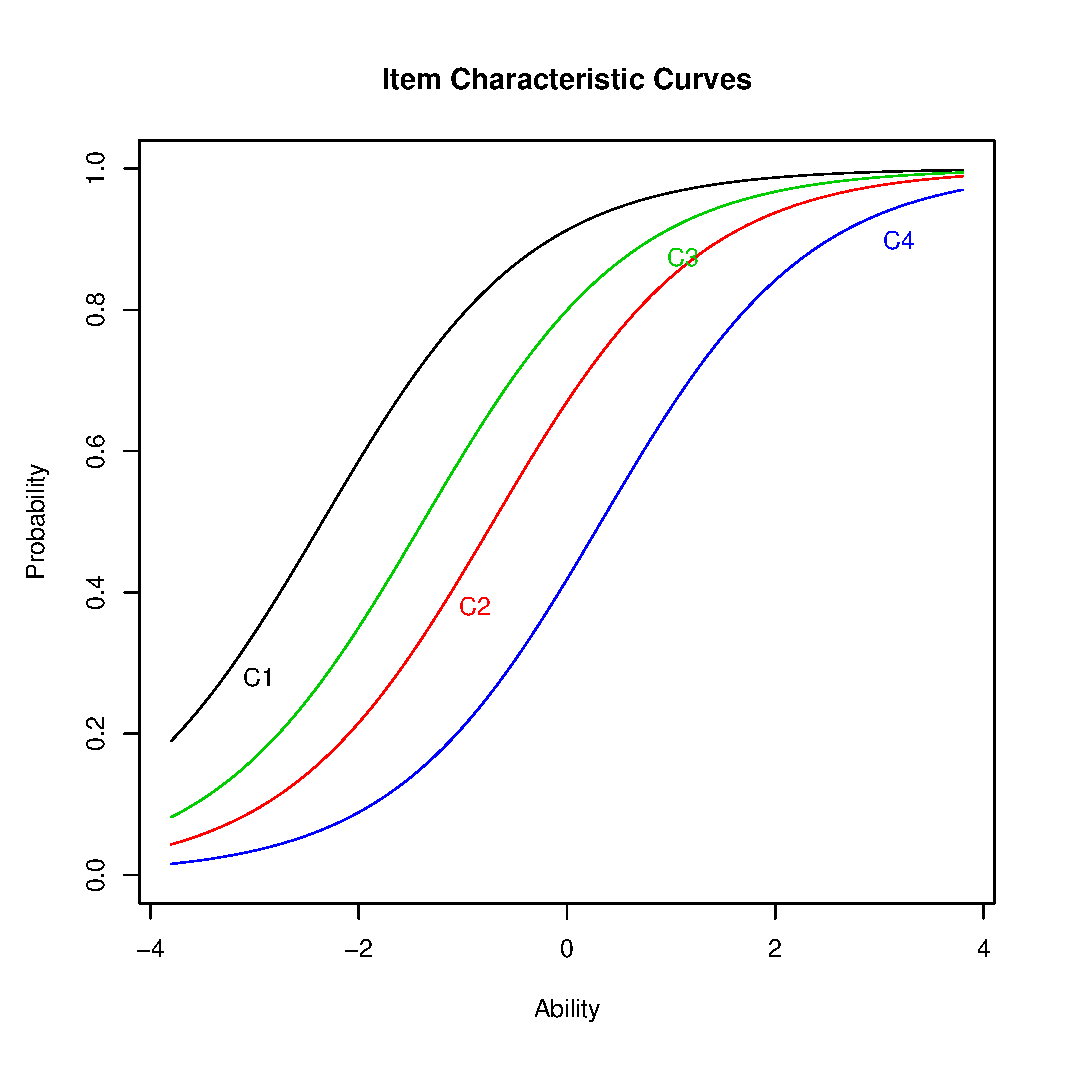
\includegraphics[scale=0.5]{icc.eps}
	\caption{ICCs of 4 items C1-C4 with different difficulties according to the Rasch model.}
	\label{fig:icc}
\end{figure}
%\end{center}

IRT models allow the simultaneous estimation of the item parameters and the examinees' abilities.
The \emph{calibration} process usually involves the estimation of item parameters from pre-test response data.
The \emph{scoring} phase deals with the estimation of the ability scores of the candidates.
Once the item parameters have been estimated, it is possible to understand how precise the test is at various ranges of the latent ability by using the test information function (TIF), which is defined as the sum of the item Fisher information for all the items in the test.
In fact, under the maximum likelihood (ML) scoring, the Fisher information is asymptotically equal to the inverse of the variance of the ML estimator as follow,

\begin{equation}
I(\theta)=\frac{1}{\text{Var}(\hat{\theta}| \theta)}.
\end{equation}

The TIF has a very favourable property that is the additivity (and hence linearity) over the items of a test.
Given a test with $k$ items, the TIF is equal to
\begin{equation}
I(\theta)=\sum_{i=1}^k{I_i(\theta)},
\end{equation}
where $I_i(\theta)$ is the item information function (IIF) for item $i$. Expressions for the IIFs can be easily derived within the framework of IRT. 

For example, for the Rasch model, the IIF of item $i$ is equal to
\begin{equation}\label{eq:infofun2pl}
I_i(\theta)=P_i(\theta)(1-P_i(\theta))=\frac{\exp^{(b_i+\theta)}}{[1+\exp^{(b_i+\theta)}]^2}.
\end{equation}
An example of IIFs for the Rasch model is shown in Figure \ref{fig:iif}. The items are maximally informative (information equal to 0.25) at the ability level corresponding to the easyness parameter.

\begin{figure}[h]
	\centering
	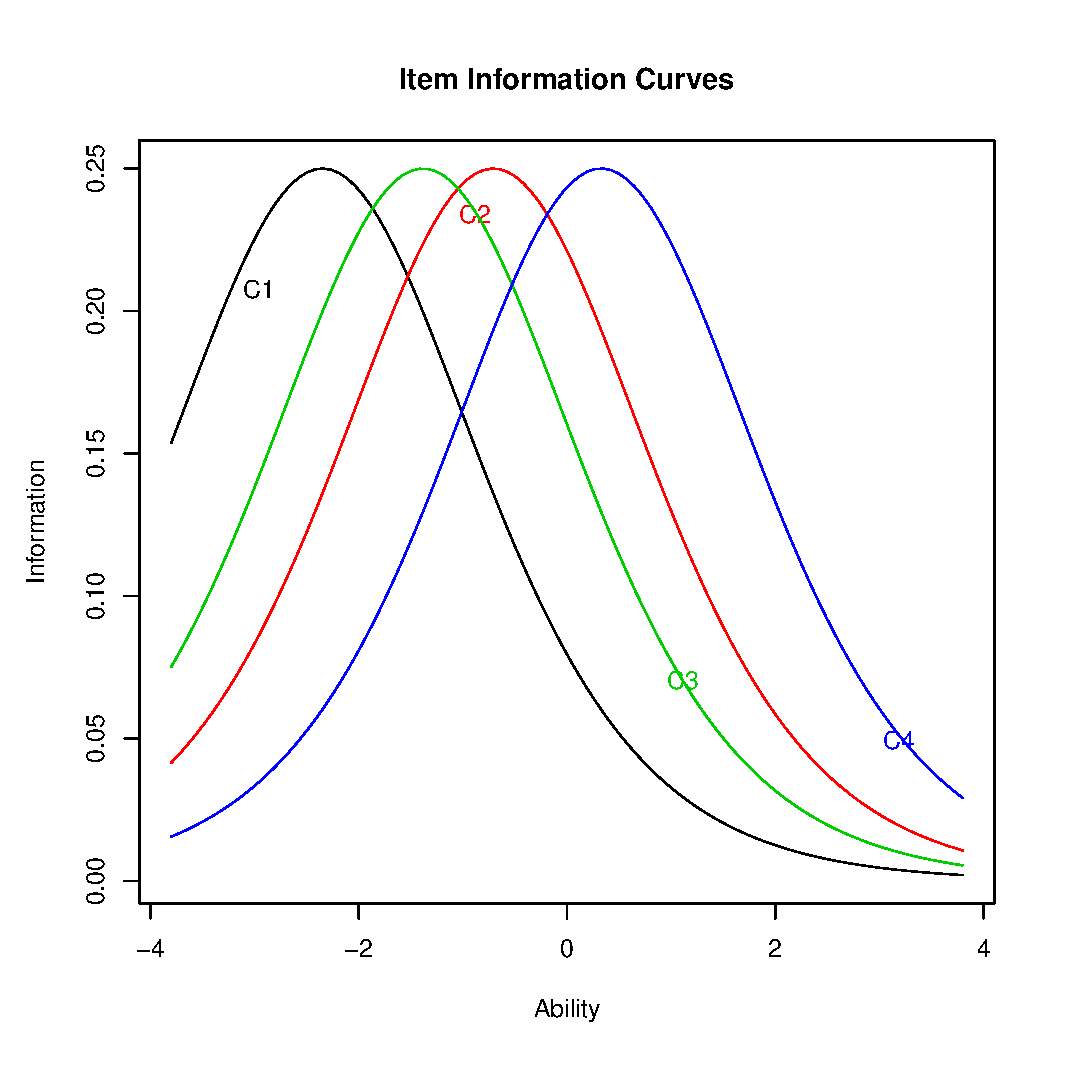
\includegraphics[scale=0.5]{iif.eps}
	\caption{IIFs of 4 items C1-C4 according to the Rasch model.}
	\label{fig:iif}
\end{figure}

Figure \ref{fig:tif} shows a test information function for a test with 10 items.
The Fisher information function is a critical element in test assembly because of its linearity and its easy interpretation.
Tests can be assembled merely through the selection of appropriate items out of an item bank, one way to do so is to use mathematical programming techniques like 0-1 linear programming (LP) or mixed integer programming (MIP) models.
Using these approaches the tests can be built by, for instance, maximizing the TIF at predefined $\theta$ points (MAXIMIN in this dissertation), or matching it with known optimal values (MINIMAX) with linear restrictions on the values of items properties.

\begin{figure}[h]
	\centering
	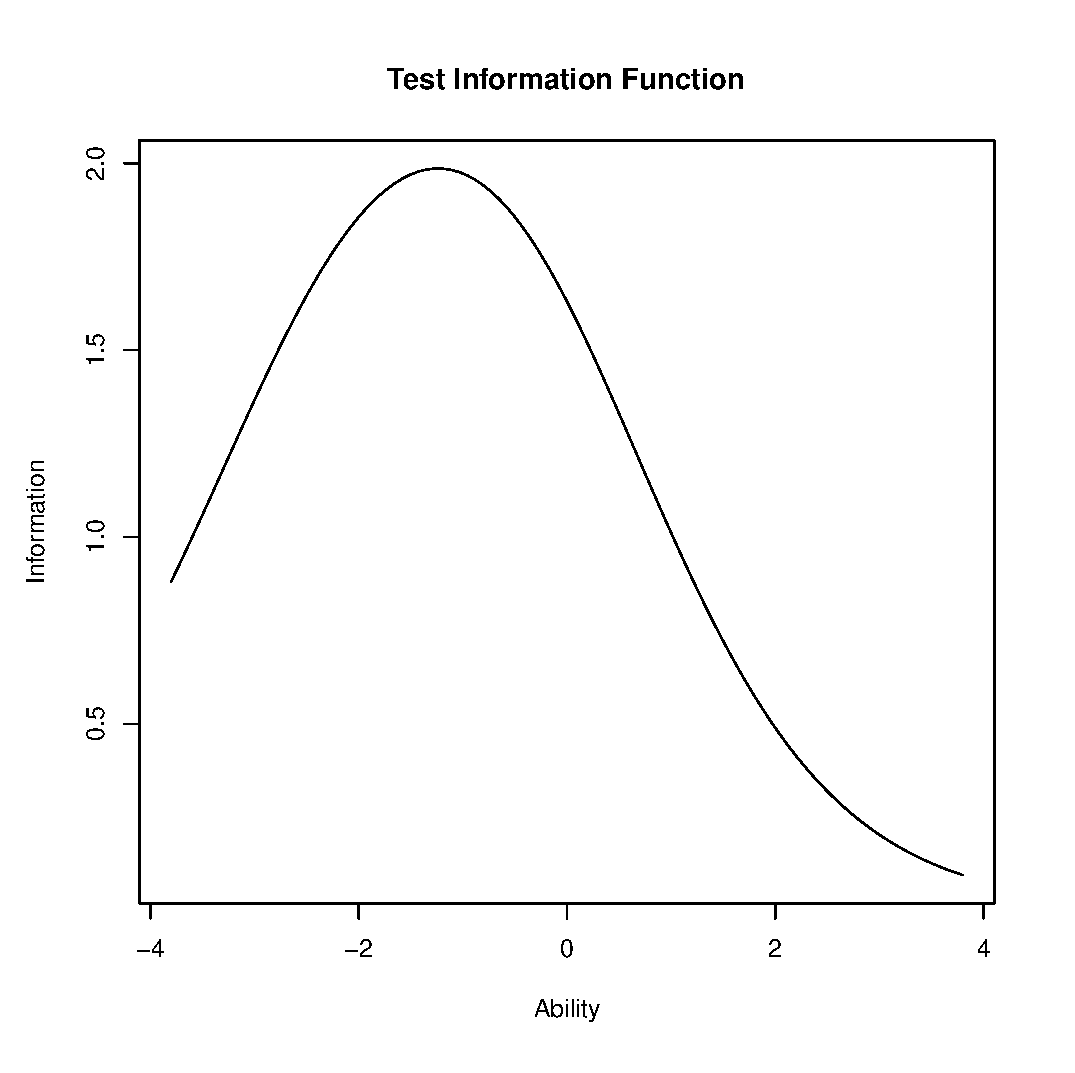
\includegraphics[scale=0.5]{tif.eps}
	\caption{An example of test information function (TIF).}
	\label{fig:tif}
\end{figure}

The 2-parameters logistic model (2PL) \parencite{birnbaum1958} is a generalization of the Rasch model.
Like the Rasch model, the 2PL assumes that the probability of a correct response to an item $i$ depends on the difference between the respondent’s trait level $\theta$ and the easiness of the item $b_i$ (note that, since $b_i$ has positive sign in our parametrization, it is interpreted as easiness).
Also, the 2PL postulates that, for every item, the association between this difference and the response probability depends on an additional item discrimination parameter: $a_i$. 
The ICC of the 2PL IRT model is given by:

\begin{equation}
P_i(\theta)=\frac{\exp(b_i+a_i\theta)}{1+ \exp(b_i+a_i\theta)}
\end{equation}

The probability of a positive response (e.g., solving an item correctly) is strictly monotonic, increasing in $\theta$ and $b_i$.
The item discrimination parameter characterizes how fast the probability of endorsing the item approaches $1.00$ with increasing trait level when compared to other items.
In other words, the model accounts for the possibility that responses to different items are not equally strongly related to the latent trait.
The discrimination parameter describes how well a particular item discriminates between examinees with different trait levels compared to other items on the test.

We decided to focus on the 2PL model because it is widely used in practical applications, \textcite{desimone2015item}

\section{Automated Test Assembly}\label{sec:ata}

In the late 1970s, the transition from paper-and-pencil to computer-based tests has begun in the United States, increasing the efficiency and the accuracy of the assessment tools.
First of all, the administration of tests by computers streamlined the process of data collection and recording, allowing to have scores immediately available and free of data entry errors.
Secondly, skills and variables that could not be assessed or measured by paper-and-pencil tests like higher-level thinking skills, complex problem-solving and response times now are quickly recorded and evaluated thanks to the computers.
The growing number of credentialing exams for allowing the practice of a profession, admission tests for granting the access to the universities and standardized national tests for comparing abilities among different settings increased the importance of the use of test scores and hence the content and statistical features of the tests became crucial for the test validity and reliability.

Automated test assembly was born in this framework where fulfilling several specific requirements on the tests such as reducing the length of the test, maximizing the precision of the ability estimates, building tests with the same difficulty level and moreover, were needed.
In practice by ATA models, a test developer can impose any content and statistical criteria, from here called constraints, by specifying them in the form of linear (in)equalities.
Also, a test developer could choose an objective function to serve as the goal for test assembly.
Therefore, the computer can find a set of test items that optimally meet these specifications.
It is clear that test assembly is at the heart of the test development process but the automatically produced test is only a first draft of tests that could then be reviewed and re-examined by committees.

At the time when the test is assembled, the input is required from  three other processes: test specification, item construction and test data
analysis.
A good test needs good specifications, good items and good data.


\subsection{The Item Bank}\label{sec:the-item-bank}
%Before entering in the test assembly framework we should fix some notation and describe how the items are usually stored in a "database" called \emph{item bank} or \emph{item pool}
Once the calibration has been done, the items and their estimated and structural properties are stored in the \emph{item bank} (or item pool). Afterwards, we can move on to the test assembly procedure in which the items will be selected depending on those distinctive characteristics.

Table \ref{fig:tabitembank} shows an example of the structure of an item bank with $I$ items, where the items are displayed by row while in the columns we find the items features, from left to right: the identifier (\textsl{ID}), the IRT difficulty parameter ($b$) together with its standard error ($b_{se}$), CTT difficulty (\textsl{p-value}), content attributes (\textsl{TYPE}, \textsl{PROCESS}, \textsl{DOMAIN}), and relational attributes that specifies if the item belongs or not to a specific set (\textsl{FRIEND SET 1}, \textsl{FRIEND SET 2}, \textsl{ENEMY SET 1}, \textsl{ENEMY SET 2}).

Examinees can get different sets of items because, thanks to the calibration via IRT, the items are set on the same scale and the examinees' scores can be compared.

\subsection{Types of Assembly Models}\label{sec:assembly-models}

Given an item bank containing a sufficient number of calibrated items, is it possible to assemble one or more test forms which features can be similar or diverge.
When we need to assemble only one test form, we are speaking about \emph{single test assembly} models while if the tests are more than one the models are for \emph{multiple test assembly}.
In particular, if the obtained ones are similar under their psychometric characteristics, they are called \emph{parallel} \footnote{Other details in Section \ref{sec:multiple-test-assembly}.}.
In this work, we will focus on the latter category of automated test assembly models.

To solve this type of problems, in the last decades, three modes of automated test assembly became prevalent: sequential, simultaneous single or multiple test assembly, and adaptive tests.
By the first two, test forms are entirely built before the administration of the test while in the adaptive framework, each test form is assembled during the testing procedure.

\subsubsection{Sequential test Assembly}

The straightforward technique for assembling single or multiple test forms is to populate the forms with items in a sequential way. This is being done by selecting items or groups of items and removing them from the pool; then the model is adapted to the new pool to try to fit the next form. 
In the case of assembling parallel forms, this method has two serious disadvantages.
First, if the forms are assembled one after the other, the value of the objective function for the solution of the model tends to decrease due to the fact that items with the best values will be selected first.
As a consequence, the forms cannot be parallel.
The second disadvantage of this approach is the possible infeasibility of later models in the sequence.
On the other hand, by this type of model, an extensive range of functions can be optimized, e.g., the linear structure of the problem can be relaxed.
Most of these problems nowadays are solved using ad hoc greedy and heuristic techniques.

\subsubsection{Simultaneous test assembly}

In the sequential approach, an incremental number of different models must be optimized in order to obtained multiple forms causing the disadvantages cited in the last paragraph.
Those can be overcome by applying simultaneous test assembly models in which the solution, and hence, the test forms, is obtained by solving only one model.
They are usually represented by 0-1 integer programming problems and solved by linear programming techniques.
The model can be reformulated as a mathematical optimization problem using decision variables.
Decision variables are defined such that the solution of the optimization problem (i.e., the set of values for which the objective function is optimal and all constraints are satisfied) identifies the best decision that can be made.
The decision variables $\{x\}_{it}$ are binary (0-1) since they represent the inclusion (1) or exclusion (0) of the item $i$ in the test $t$.
In the last decades, the algorithms needed to solve such optimization problems were improved, and nowadays, powerful implementations of them are available as commercial or open-source software.

\subsubsection{Adaptive tests}

In the adaptive approach, one item is optimally picked from the pool at a time.
The person's ability estimate is updated during the test, and the next item is chosen to be maximally informative at the last ability update.
The test is then tailored to the candidate.
Because ability estimates converge to the person's true ability level, the item selection improves during the test and the ideal test with maximum information at the person's true ability level is approached.
In the early 1990s, computerized adaptive testing (CAT) was implemented in large-scale testing programs, and nowadays large numbers of subjects are tested worldwide using this type of test assembly.
One of the most important benefits of this method is that it's more efficient, i.e., it is possible to get more precise ability estimates with fewer items than the previous standard approaches, but at the cost that it's quite impossible to ensure the congruence between tests since all the test takers will get a different set of items from the pool.

The description of different approaches to assemble tests is not finished here.
Because of its advantages, the approach dealt with in this report is the simultaneous tests assembly mode.
In Section \ref{sec:single-test-assembly} and Section \ref{sec:multiple-test-assembly} we introduce the reader to the standard test assembly models used to build first, a single test form and secondly, as a generalization, multiple test forms.

\subsection{Single Test Assembly}\label{sec:single-test-assembly}

As already discussed, a new testing program starts with formulating the set of specifications for the test to be met, that here we call \emph{desiderata}.
Sometimes they are verbally expressed as a set of learning objectives or a list of dos and don'ts for the test developer, but they can also be well-structured in tables specifying how many items should have certain content or, even better, the distribution of items according to their specific characteristics.

Once the desiderata have been collected, they must be translated into a standardized language used in test assembly problems.
The standard form of these problems is composed of an \emph{objective function} to be optimized subject to several \emph{constraints}, where the latter define a possibly feasible set of tests for a given item bank, and the former expresses our preferences for the tests in this feasible set.
If the specifications have been formulated in a simple, concise, but complete way, it is possible to determine whether they are objectives or constraints.
These requirements are crucial for a correct translation of the desiderata into the standard language for test assembly problems: disambiguations and possible complications may arise in test design if these principles are not satisfied.
An example of verbal test specifications is described in the Table \ref{tab:exspec}, which is partially extracted from \textcite{VDL2005}.

\begin{table}
	\centering
	\begin{tabular}{|ll|}
		\hline & \\
		1. & Average \textit{p}-value of the test between .40 and .60 \\
		2. & Number of items on applications equal to 24 \\
		3. & Reliability of the test should be as high as possible \\
		4. & Items 73 and 100 never in the same test \\
		5. & Test information function as close as possible to the target \\
		6. & Items 33, 45 and 12 must be in the same test \\
		& \\
		\hline
	\end{tabular}
	\caption{Example of desiderata.}\label{tab:exspec}
\end{table}

The specifications in Table \ref{tab:exspec} may represent either objectives or constraints; for example, points 1,2,4 are constraints while 3 and 5 are objectives.
It is clear now that the objectives involve maximize or minimize some attributes, such as minimize the gap between the test information function at some $\theta$ point to its target (5) or maximize the reliability of the test (3) and on the other hand constraints impose a bound on an attribute of the test or of the items, such as limiting the difficulty of the test (1), fixing the number of items having specific characteristics (2) or considering enemy sets (4) or also item (friend) sets (6). An exhaustive classification of specifications together with examples of not well-expressed desiderata can be found at pages 34-39 of \textcite{VDL2005}.

\subsubsection{Standard form of a test assembly problem}

If a set of desiderata is well specified, they can always be represented in the standard form of Table \ref{tab:stform}.

\begin{table}
	\centering
	\begin{tabular}{|ll|}
		\hline    & \\
		optimize & \textit{Objective function} \\
		subject to & \\
		& \textit{Constraint 1} \\
		& \textit{Constraint 2} \\
		& $\vdots$ \\
		& \textit{Constraint N} \\
		& \\
		\hline
	\end{tabular}
	\caption{Standard form of a test assembly problem.}\label{tab:stform}
\end{table}

Only one objective can be optimized at a time; if we have more than one function to optimize some tricks can be applied to transform the objectives into constraints. On the other hand, there is no upper limit for the number of constraints, provided our solver can handle the problem.
If, at least one combination of items that meets all the constraints do exist, the set of these combinations is called \emph{feasible set}; if this set is empty, we say that the model in \emph{infeasible}.
The subset of tests in the feasible set that optimizes the objective function is called \emph{optimal feasible solution}.

\subsubsection{Decision variables}

Modelling a test assembly problem does not imply only defining objectives and constraints, but we also need the so-called \emph{decision variables} which represent the possible combination of items that compose the test form in a mathematical formulation.
If we need to assemble a single test from a pool of $I$ items, we can choose as decision variables $I$ binary variables in the form:
\begin{equation*}
x_{i}=
\begin{cases}
1 & \mbox{if item }i \mbox{ is in the test},\\
0 & \mbox{otherwise}.
\end{cases}
\end{equation*}

We can also write the $x_i$ in an algebraic way using the vector $x$ of length $I$. 
Therefore, we have $2^I$ possible combinations of values the vector $x$ can take.
These combinations decrease in number if we add constraints to the model.
In the following Section, we will also use non binary variables like integer o continuous, which are often useful to reduce the number of objectives in the problem.
Once the decision variables have been identified, the process of modelling a test assembly problem goes through the steps of modelling the constraints and objectives and solving the model looking for an optimal solution.
In the following Section, we will present the basic formulations for some common types of constraints and objectives. The last step consists of solving the model by using a computer program which implements some mathematical or numerical algorithms.

\subsubsection{The model for assembling a single test}

The models presented in this Section are based mainly on item response theory attributes. 
Here, we will make an almost exhaustive list of categories of constraints that can be added to a model for single test assembly together with possible objective functions.

The standard model for the assembly of a single test with a generic quantitative objective from a pool of $I$ items indexed by $i=1,\ldots,I$ is
\begin{subequations}\label{eq:singClassTest}
	
	\begin{equation}\label{eq:Sobj}
	\mbox{optimize } {\sum_{i=1}^I q_i x_{i}} \quad \mbox{(objective)}
	\end{equation}
	subject to    
	\begin{alignat}{4}
	\label{eq:Scat}
	&n^{\min}_{c} \ &\le & \sum_{i \in V_c} x_i &\le \ & n^{\max}_{c}, \ & \forall c \quad & \mbox{(categorical constraints)}\\
	\label{eq:Squan}
	&b^{\min}_{q} \ &\le & \sum_{i=1}^I q_i x_i &\le \ & b^{\max}_{q}, \ &              \quad & \mbox{(quantitative constraints)}\\
	\label{eq:Slen}
	&n^{\min}      \ &\leq & \sum_{i=1}^I x_i &\le \ & n^{\max},      \ &             \quad & \mbox{(test length)}\\
	\label{eq:Sene}
	&    \ & & \sum_{i \in V_e} x_i&\le \ & 1,              \ & \forall e \quad & \mbox{(enemy sets)}.
	\end{alignat}
	
	Then, definition of variables
	\begin{equation*}\label{eq:SDV2}
	x_i \in \{0,1\}, \ \forall i \quad \mbox{(decision variables)}.
	\end{equation*}
	\label{eq:Smod}
\end{subequations}
where the sums in the constraints may be bounded only on one side, in which case we only need one of the two inequalities.

For a qualitative variable, we use $V_c$ to represent the set of indices of the variable of the items in subset $c$.
Allowing the test to have several items with specific qualitative attribute represented by $V_c$ between $n^{\min}_{c}$ and $n^{\max}_{c}$ means adding a \emph{categorical constraint} to the model.
An example of a categorical constraint is ``the test must contain at least 10 items in problem-solving'', where the set of items in the pool that has the attribute ``problem solving'' is represented by $V_\text{problem solving}$ and $n^{\max}_\text{problem solving}=10$.

On the other hand, if we want to bound the value of a quantitative variable (i.e. that can take numerical values) addressed by the symbol $q$ between the values $b^{\min}_{q}$ and $b^{\max}_{q}$ we are constraining the model adding a \emph{quantitative constraint} where $q_i$ is the value that the item $i$ takes for that variable.
Suppose we want to assemble a test with the following criterion ``the maximum of words must be 300'', $q_i$ will serve as the number of words displayed by the item $i$ and $b^{\max}_{q}=300$.

The interpretation of the \textit{test length} constraint is straightforward as it is a special case of a quantitative constraint where $q_i=1$ for each $i=1,\ldots,I$.

If there are \textit{enemy sets} in our pool, then the items in one of these sets, called $V_e$, cannot be picked together, e.g., the desideratum ``items 23 and 46 cannot be in the same test'' means that items 23 and 46 are enemies and both are in the enemy set $V_e$.
Therefore, the sum of the corresponding decision variables $x_{23}$ and $x_{46}$ cannot be more than 1.

\subsubsection{Item sets}\label{sec:item-sets}

Tests with sets of items organized around common stimuli (known as item sets or friend sets) are popular because of the efficiency of their format.
By combining more than one item with the same stimulus, we can ask questions using more complex stimuli, such as reading passages, descriptions of cases, or problems with data in a set of tables or graphs, without having to sacrifice too many items for the test to meet the time limit.
However, the presence of such sets in the item pool complicates the process of assembling the test.
In particular, if the items are grouped in $S$ item sets, or stimuli, indexed by $s$, there are three ways to deal with this problem \parencite[see][]{VDL2005}.

\begin{itemize}
	\item The \textit{power set method} that consists in summarizing all the quantitative and qualitative attributes by summing or averaging them taking as groups the item sets; if we only need to constraint the test at the set/stimuli level the problem decreases in size since you don't have $I$ decision variables anymore but just $S$. This method is not efficient if you have variables that cannot be summarized, such as standard errors and if you want to keep some constraints at item level since you need to consider again the original decision variables $x_i$ increasing the size of the model.
	\item The \textit{pivot-item method} in which each set is represented by a pivot decision variable $x_{i^*_s}$ arbitrarily chosen. Therefore, we can use the variable for a pivot item as a carrier of the attributes of both its stimulus and item set, and we can drop the stimulus variables in the model.
	\item The \textit{two-stage method} that is a sequential approach with two phases, in the first, stimuli are selected and secondly, the model chooses the items with those stimuli.
	
\end{itemize}
Given the earlier warnings about sequential approaches we do not suggest the two-stage method and since all the variables in our item bank are summarizable (e.g., the item information function is additive, so it is possible to sum it for all the items in the stimulus) we prefer to adopt the power set method which helps to decrease the size of the problem.
\par{
	The power-set formulation needs a phase of preprocessing of the item bank.
	Instead, for the formal representation of the model, we refer to \textcite[Section 7.2, ][]{VDL2005}.}

\subsubsection{Single test MINIMAX}\label{sec:single-test-minimax}

Once we defined all the constraints, and checked that the model is feasible, we need to choose an objective to optimize.
A first option is to choose absolute targets for the TIF, targets are the values that a goal TIF assumes on a fixed number of $\theta$ points along the $\theta$ scale, these values must be chosen by test specialists who knows how much precision is required to estimate the abilities of the students at each ability level.
That is the reason why absolute targets are used almost exclusively when tests are assembled to be parallel with respect to a known reference test. 
Formalizing this requirement in the standard form of test assembly models will produce a multi-objective test assembly problem that must be reformulated using the MINIMAX approach explained below.

In particular, with the following addition to the model \eqref{eq:Smod} we ask that the TIF of the resulting test approximates with minimum negative and positive deviations (i.e., with the highest precision) the chosen goal TIF in a finite set of points $V$ on the $\theta$ scale, which we denote as $T_{k}$ with $k \in V$:
\begin{subequations}[intermezzo]
	\begin{equation}
	\mbox{minimize } \ y \quad \mbox{(objective)}
	\end{equation}
	subject to
	\begin{alignat}{2}
	\label{eq:SMINIMAX1}
	\sum_{i=1}^I I_i(\theta_{k}) x_{i} & \le T_{k}+ y, &\ \forall k \in V \\
	\label{eq:SMINIMAX2}
	\sum_{i=1}^I I_i(\theta_{k}) x_{i} & \ge T_{k}- y, &\ \forall k \in V
	\end{alignat}
	\begin{equation*}
	y \ge 0.
	\end{equation*}
	\label{eq:SMINIMAX}
\end{subequations}
More $\theta$ points we choose more the TIF of the assembled test will meet the auspicable one, usually 3-5 points are enough to have a good approximation.

\subsubsection{Single test MAXIMIN}\label{sec:single-test-maximin}
If a reference test or absolute targets are not available, an alternative approach is trying to achieve the best predictive validity for the test, that is maximizing the TIF in some chosen theta points.
This goal can be met not only setting the location of the peaks of the TIF but also defining its shape in the entire $\theta$ scale, which is to say imposing relative targets.

So, denoting with $R_k$ the relative targets for each $\theta_k$ with $k$ in the chosen set $V$ of ability points in which we want to control the shape of the TIF, we must fix one of the relative targets to a value (e.g. $R_1=1$) and all the other target values must be adjusted correspondingly trying to reproduce the wanted shape.

Like the absolute target model, this method leads to having more than one objective function and also, in this case, it is possible to rely on a simplifyed approach called MAXIMIN.
The model can be formalized as follows:
\begin{subequations}\label{eq:MAXIMIN}
	\begin{equation}
	\mbox{maximize } \ y \quad \mbox{(objective)}
	\end{equation}
	subject to
	\begin{equation}\label{eq:SMAXIMIN1}
	\sum_{i=1}^I I_i(\theta_{k}) x_{i} \ge yR_{k}, \ \forall t,k \in V
	\end{equation}
	\begin{equation*}
	y \ge 0.
	\end{equation*}
	\label{eq:SMAXIMIN}
\end{subequations}
Also here, the practice suggests that the minimum number of $\theta$ points in which maximizin the TIF must be 3 or 5.

\subsection{Multiple Simultaneous Test Assembly}\label{sec:multiple-test-assembly}
%\par The models presented in the previous chapters are to assemble single test, however

In order to discourage the phenomenon of cheating, it is necessary to administer different items to the test takers. This can be achieved building more than one test form that contains different items preserving some overall mutual psychometric features, such as the same test difficulty or same content structure such as the same percentage of items of a certain stimulus. These tests are called \emph{parallel} (or interchangeable) and the procedure aimed to perform this task is called ``multiple test assembly''. In particular, test forms are defined to be \emph{weakly parallel} if their information functions are identical \textcite{same77}. On the other hand, test forms are \emph{strongly parallel} if they have the same test length and the exact test characteristic function \textcite{Lord80}.

As a consequence, we typically have problems with more objectives than those presented in Section \ref{sec:single-test-assembly} for a single test assembly. For example, if we assemble $T$ tests and each test has to meet a target for its information function at $K$ ability points (the same points for each test $t$, with $t=1,\dots, T$), the problem has at least $T \times K$ objectives. However, these sizeable multi-objective test assembly problems can be solved using a direct generalization of the approaches for single test assembly. In the following, we will present a general model for simultaneous assembly of a set of tests (that is, as a solution to a single model) that produces an optimal solution.
This type of assembly requires a reorganization of the problem using a different version of the decision variables. These variables have double indices\footnote{We use a matrix representation only for a better visual idea, actually they are still vectors but of bigger size.}, one for the items in the pool and the other for the test forms. For the current problem, the variables become

\begin{equation*}\label{eq:MDV}
x_{it} =
\begin{cases}
1, & \mbox{if item } i \mbox{ is assigned to test }t\\


0, & \mbox{otherwise}
\end{cases}
\end{equation*}
for all $i$ and $t$.
Like before, we need to complement these variables with a set of constraints that keep their values consistent.
The adapted single test assembly model is presented here followed by constraints that arise only in the case of multiple test assembly.

\subsubsection{The model for assembling multiple tests}

Using the above decision variables, any model for a single test can be reformulated as a model for multiple tests. To illustrate this statement, we reformulate the standard model for a single test in \eqref{eq:Sobj}-\eqref{eq:Sene}.
The model is

\begin{subequations}\label{eq:classTest}
	\begin{equation}\label{eq:Mobj}
	\mbox{optimize } \sum_{t=1}^T{\sum_{i=1}^I q_{it} x_{it}} \quad \mbox{(objective)}
	\end{equation}
	subject to    
	\begin{alignat}{4}
	\label{eq:Mcat}
	&n^{\min}_{ct} \ &\le & \sum_{i \in V_c} x_{it} &\le \ & n^{\max}_{ct}, \ &\forall c,t \quad & \mbox{(categorical constraints)}\\
	\label{eq:Mquan}
	&b^{\min}_{qt} \ &\le & \sum_{i=1}^I q_i x_{it} &\le \ & b^{\max}_{qt}, \ & \forall t \quad & \mbox{(quantitative constraints)}\\
	\label{eq:Mlen}
	&n^{\min}_t \ &\leq& \sum_{i=1}^I x_{it} &\le \ & n^{\max}_t, \  & \forall t \quad &\mbox{(test length)}\\
	\label{eq:Mene}
	&    & & \sum_{i \in V_e} x_{it}&\le \ & 1,   \  & \forall t,e \quad &\mbox{(enemy sets)}
	\end{alignat}
	
	Then, the definition of variables
	
	\begin{equation*}\label{eq:MDV2}
	x_{it} \in \{0,1\}, \ \forall i,t \quad \mbox{(decision variables)}
	\end{equation*}
	\label{eq:Mmod}
\end{subequations}

The changes in \eqref{eq:Mmod} relative to the original model in \eqref{eq:Sobj}-\eqref{eq:Sene} are:
\begin{enumerate}
	\item the replacement of the variables $x_i$ by $x_{it}$;
	\item the extension of the objective function to the case of $T$ tests;
	\item the indexing of the bounds in the constraints by $t$ to enable to assemble tests with different specifications.
\end{enumerate}
The generalization of the objective function in \eqref{eq:Mobj} is simple and consists of taking an (unweighted) sum over the tests.

\subsubsection{Item sets}
The power-set method presented in \ref{sec:item-sets} can be easily generalized to the case of multiple tests assembly, for the sake of brevity we prefer to skip the details and still refer to the van der Linden book \textcite{VDL2005}, Section 7.2.
\subsubsection{Item use}\label{sec:item-use}
If we want to control the minimum or the maximum number, respectively $n^{\min}_i$ and $n^{\max}_i$, of tests in which an item $i$ can be assigned, we have to consider the following constraints:
\begin{subequations}[resume]
	\begin{equation}\label{eq:Mmod:Muse}
	n^{\min}_i \le \sum_{t=1}^T x_{it} \le n^{\max}_i, \ \forall i, \quad \mbox{(item use)}
	\end{equation}
\end{subequations}

\subsubsection{Test overlap}\label{sec:test-overlap}
Since we are creating more than one test form we are not only concerning the properties of each form singularly but also the relationship between them, one of these is the \emph{test overlap}, that is the number of items two forms share.
Sometimes, it is not important to control for this specification, especially if an item use constraint has been fixed.
However, if we do not want any overlap between all the pairs, as an example, we have to add these constraints to \eqref{eq:Mmod}
\begin{subequations}[resume]
	\begin{equation}\label{eq:Mmod:noOL}
	\sum_{t=1}^T{x_{it}} \leq 1, \ \forall i, \quad \mbox{(no overlap)}
	\end{equation}
\end{subequations}

The latter is not enough if the test developer wants to keep the same but not a null level of overlap between all the possible pairs of tests.
In this case, the model has to be modified not only adding new constraints but also a substantial number of variables (luckily binary).
In particular, controlling for test overlap means adding quadratic constraints of the form:
\begin{subequations}[intermezzo]
	\begin{equation*}
	o^{\min}_{tt'} \le \sum_{i=1}^I{x_{it}x_{it'}} \le o^{\max}_{tt'}, \ \forall t \neq t', \quad \mbox{(fixed overlap NON LINEAR)}
	\end{equation*}
\end{subequations}

Those types of constraints must be linearized in order to use the standard LP solvers, so they must be replaced by the following variables
\begin{equation*}
z_{itt'}=
\begin{cases}
1 & \mbox{if item }i \mbox{ is both in test }t \mbox{ and test } t' \mbox{ (i.e. }x_{it}=x_{it'}=1 \mbox{)} \\
0 & \mbox{otherwise}.
\end{cases}
\end{equation*}

This modification increases the size of the model of $I*{{T}\choose{2}}$ binary variables.
Together with the new variables, the constraints must be replaced by
\begin{subequations}[resume]
	\begin{equation}
	o^{\min}_{tt'} \le \sum_{i=1}^I{z_{itt'}} \le o^{\max}_{tt'}, \ \forall t \neq t', \quad \mbox{(fixed overlap LINEAR)}
	\end{equation}
	Integrality constraints:
	\begin{alignat}{2}
	\label{eq:Mmod:Mic1}
	z_{iit'} & \ge x_{it}+x_{it'}-1 \ & \forall i,t \neq t'\\
	\label{eq:Mmod:Mic2}
	2 z_{iit'} & \le x_{it}+x_{it'} \ & \forall i,t \neq t'\\
	\nonumber
	%\label{eq:Mmod:MolDV}
	z_{itt'} & \in \{0,1\}, \ & \forall i,t \neq t'     
	\end{alignat}
	
\end{subequations}
The last two constraints are necessary to keep the values of $z_{itt'}$ consistent with their definitions.

\subsubsection{Multiple MINIMAX}

An example of an objective for multiple test assembly is the generalization of the MINIMAX principle presented in \ref{sec:single-test-minimax}, formally
\begin{subequations}
	\begin{equation}
	\mbox{minimize } \ y \quad \mbox{(objective)}
	\end{equation}
	subject to
	\begin{alignat}{2}
	\label{eq:MMINIMAX1}
	\sum_{i=1}^I I_i(\theta_{kt}) x_{it} & \le T_{kt} + w_ty, \ & \forall t,k \in V_t\\
	\label{eq:MMINIMAX2}
	\sum_{i=1}^I I_i(\theta_{kt}) x_{it} & \ge T_{kt} - w_ty, \ & \forall t,k \in V_t
	\end{alignat}
	\begin{equation*}
	y \ge 0
	\end{equation*}
	\label{eq:MMINIMAX}
\end{subequations}
where the target values $T_{kt}$ are indexed by $t$ to allow us to set different targets for different tests. Besides, a different set of values $V_t$ for each test can be given; we can specify the target values at a different set of $\theta$ values for each test. Finally, we have added weights $w_t$ to have the option of weighting deviations from target values differently for several tests. If our goal is to assemble parallel tests, the targets and weights will be equal for all $t$.

\subsubsection{Multiple MAXIMIN}

The approach used in Section \ref{sec:single-test-maximin} may be generalized to the case of multiple test assembly with this mix of objective and constraints
\begin{subequations}\label{eq:maximinmodel}
	\begin{equation}
	\mbox{maximize } \ y \quad \mbox{(objective)}
	\end{equation}
	subject to
	
	\begin{equation}\label{eq:MMAXIMIN2}
	\sum_{i=1}^I I_i(\theta_{kt}) x_{it} \ge yR_{kt}, \ \forall t,k \in V_t
	\end{equation}
	\begin{equation*}
	y \ge 0,
	\end{equation*}
	\label{eq:MMAXIMIN}
\end{subequations}

where the $R_{kt}$ may be chosen equal between tests, i.e. $R_{kt}=R_{k't'}$ with $t \ne t'$ and $\forall k=k'$ ensuring the parallelism.
%where the $\epsilon_{kt}$ may be chosen to ensure that the TIFs of upcoming tests are inside a certain interval around the maximum possible, it may also be equal to 0 for all $k$ and $t$ and therefore the constraints \eqref{eq:MMINIMAX2} will be withdrawn. Usually, the $\theta$s in the constraints are taken as the points in the ability continuum in which we want the TIFs are maximized.

\subsection{Lagrange relaxation}\label{sec:lagrange}

In the previous sections, we introduced the classical linear models for test assembly formalized in the book \textcite{VDL2005}. In the chapeter 4.3 of this book, an approach to approximate those models by means of Lagrange multipliers is briefly mentioned, that is a \emph{Lagrange relaxation} of the test assembly model \eqref{eq:classTest}.
This method is beneficial in case of infeasibility, a situation very common in practice when there is a large number of constraints or optimization variables. For example, when a large-scale test assembly model of the type \eqref{eq:classTest} is given to a MILP solver, it may happen that a set of tests that meets all the constraints cannot be found, even if the user imposed time limit is very long. This is a very big issue for the test assembler because, usually, the solver just says that the problem in infeasibile without returning any diagnostic, so he/she does not know which constraints made the problem infeasible and he/she does not have any assembled test in his/her hands, not even a barely good one. 

The Lagrange relaxation \parencite{fisher1981lagrangian} overcomes this issue by including in the objective function the absolute deviation, called \emph{violation}, of the incumbent from the constraints. In this way, we try to solve a simplified version of the problem, and we obtain an upper bound for the optimal solution of the initial problem. Even if the problem is highly infeasible, the solver returns the most feasible combination of variables that maximizes the modified objective function.
Thus if we have the most general optimization model:

\begin{subequations}\label{eq:optModel}
	
	\begin{equation}
	\mbox{maximize } {f(x)} \quad \mbox{(objective)}
	\end{equation}
	subject to    
	\begin{alignat}{3}
	&g_m(x) &\le \ & 0 , \ & \forall m \quad & \mbox{(constraints)}
	\end{alignat}
	\begin{equation*}
	x \in \mathbb{R}^d, \ \quad \mbox{(decision variables)}
	\end{equation*}
	
\end{subequations}
Its Lagrange relaxation will be:
\begin{subequations}\label{eq:LRoptModel}
	
	\begin{equation}
	\mbox{maximize } {f(x)-\lambda\sum_m g_m(x)} \quad \mbox{(objective)}
	\end{equation}
	
	\begin{equation*}
	x \in \mathbb{R}^d, \quad \mbox{(decision variables)}
	\end{equation*}
\end{subequations}
where $f()$ ad $g()$ are generic functions from $\mathbb{R}^d$ to $\mathbb{R}$ and $\lambda$ is a constant called the Lagrange multiplier, it has the role to weight the violations of the constraint in the new objective function.
We opt for a modification of the previous model to allow the violations to interfere in the optimization only when the constraints are not met. The \eqref{eq:LRoptModel} will become:
\begin{subequations}\label{eq:LRoptModelmax0}
	\begin{equation}
	\mbox{maximize } {f(x)-\lambda\sum_m \max{[0,g_m(x)]}} \quad \mbox{(objective)}
	\end{equation}
	
	\begin{equation*}
	x \in \mathbb{R}^d, \quad \mbox{(decision variables)}
	\end{equation*}
\end{subequations}

In the field of neural networks, $\max{[0,g_m(x)]}$ is called \emph{RELu} activation function and, in machine learning, it is mentioned as \emph{hinge loss} and it is used for training classifiers. In this context this function serves a different purpose but we will continue to use this names as a reference.

In the case of test assembly, the relaxation of the classical model \eqref{eq:classTest} is still linear.
We summarise this approach by an example of the Lagrange relaxation applied to a single test assembly model of the form \eqref{eq:singClassTest} with an objective function to maximize.
Suppose we have two set of indices $m_u \in M_u$ and $m_l \in M_l$ for upper and lower bound constraints and $m \in M_u \cup M_l$. we can rewrite the relaxed version of the model \eqref{eq:singClassTest} as follows: 
\begin{subequations}\label{eq:LRsingClassTest}
	
	\begin{equation}
	\mbox{maximize } {\beta\sum_{i=1}^I q_i x_{i}-(1-\beta)\sum_{m=1}^{m_u+m_l}{z_m}} \quad \mbox{(objective)}
	\end{equation}
	subject to    
	\begin{alignat}{3}
	\label{eq:LRgenConupper}    & \sum_{i=1}^I c_{i{m_u}}x_i - ub_{m_u} &\le \ & z_{m_u}, \ & \forall m_u \quad & \mbox{(generic constraints with upper bound)}\\
	\label{eq:LRgenConlower}    & -\sum_{i=1}^I c_{i{m_l}}x_i + lb_{m_l} &\le \ & z_{m_l}, \ & \forall m_l \quad & \mbox{(generic constraints with lower bound)}
	\end{alignat}
	\begin{equation*}
	x_i \in \{0,1\}, \ \forall i \quad \mbox{(decision variables)}
	\end{equation*}
	\begin{equation*}
	z_m \in \mathbb{R}^+, \ \forall m \quad \mbox{(violations)}
	\end{equation*}

\end{subequations}

Notice that any of the linear constraints showed in the previous subsections can be represented as a generic constraint either of the form \eqref{eq:LRgenConupper} or \eqref{eq:LRgenConlower}.
The definition of $z_m$ as a positive real number let the solver look for solutions that makes the sum of $z_m$ go to zero and hence satisfy all the constraints. 

To help the test assembler to control the trade-off between optimality and feasibility of the final solution, we let them to choose the Lagrange multiplier $(1-\beta)$, where $0\leq\beta\leq1$.
For example, if the assembler prefers a solution more accurate in the ability estimation sacrificing the fulfillment of tougher constraints they might choose a $\beta>0.5$ Viceversa if they need to respect all the requirements in the desiderata they will select a lower $\beta$.
For a balanced solution, the $\beta$ must be equal to $0.5$.
In chapter \ref{sec:CCATA} we will refer to the model without Lagrange relaxation \eqref{eq:optModel} as the \emph{strict} model, instead, the model of type \eqref{eq:LRoptModel} will be called \emph{relaxed} model.






	\label{key}% Chapter 1

\chapter{IRT item parameter calibration in Julia} % Main chapter title
\label{ch:Julia}

Item response theory (IRT) models, already introduced in Chapter \ref{sec:TestTheories}, are a class of statistical models which are intended to describe the response behaviors of individuals to a set of questions which have a discrete outcome. The item responses are observable manifestation of underlying traits or constructs not directly measured which are called \emph{latent} variables. In the framework of latent class analysis, IRT models hyphotesize the latent variable as continuous, instead, the observed variables are patterns of discrete-valued responses, in particular they can be dichotomous (correct/incorrect) or polythomous. Common assumptions in IRT are the unidimensionality of the latent trait is  since it's considered to be enough to describe the individuals propensity to endorse the items in the survey and conditional indipendence of the probability of a correct response given a certain level of ability. Moreover, IRT models can be seen as a specific type of fixed-effect or random-effect model \parencite{fox2006fixed} or, changing the parametrization, they become a particular case of latent regression models \parencite{von2010stochastic}. 

Once the model is set, the parameters and the latent variables must be estimated. For example in the 2-parameter logistic (2PL) model \parencite{BockMislevy1982}, easiness and discrimination power of the items must be quantified. Several algorithms to retrieve the estimates exist, most of them are based on the expectation maximization (EM) paradigm and differ on the way in which the expectation is approximated and in how the optimization model is solved, some examples are the joint maximum likelihood (JML) \parencite{lord1968statistical}, the marginal maximum likelihood (MML) \parencite{drasgow1989evaluation}, the stochastic EM algorithm \parencite{fox2003stochastic} and the Bayesian methods which adopt monte carlo Markov chain (MCMC) or Gibbs samplers technique to approximate and maximize the posterior of the latent variable \parencite{matteucci2012prior}. 

In this work the unidimensional model, dichotoumous response data and MML estimation method will be taken into account. The latter is widely recognized to outperform the JML and MCMC in terms of consistency of the estimates \parencite{andersen1977sufficient, neyman1948consistent} and computational time  \parencite{patz1999applications} respectively. Unlike the joint maximum likelihood estimation technique, which treat each of the responses as separate observational units, the MML estimation treats only the individuals as such. To accomplish this the MML technique assumes that the latent traits are random effects sampled from some continuous distribution, usually discretized in order to compute the expected value of the likelihood in the first step of the EM algorithm, called \emph{E-step}. In this context, the linear representation allows to perform faster computations of the involved functions since some arrays are computed only once and reused in all the iterations. Another advantage is the use of simple linear algebra transformation such as matrix/matrix or matrix/vector multiplications which are extremely fast in modern programming languages\footnote{The \texttt{BLAS} routines are an example of very fast implementation of linear algebra operations. See  \url{http://www.netlib.org/blas/}}. 

Moreover, since we chose to work in the \texttt{Julia} environment due to its suitability for numerical and computational tasks, we also developed a calibration algorithm for the case of the unidimensional 2PL already introduced in Chapter \ref{ch:ATA}. The cubic-spline interpolation-extrapolation method \parencite{birkhoff1960smooth} is used to recompute the masses of the rescaled observed ability distribution at the predefined theta points. The details of the applied methodology are provided in Section \ref{sec:estimation} together with a software benchmarking which compare the performance of our algorithm to the \texttt{R} \texttt{mirt} package.

Finally, a full reading of this chapter will suggest to both practitioners and scholars a framework for building a pre-test design without knowing the item parameters and for doing a simulation study for testing the performance of an estimation method. The framework is described both in Section \ref{sec:semcalbs}. The package together with the code and the detailed results we obtained are available at \url{https://github.com/giadasp/IRTCalibration}\footnote{Accessible only prior request to \href{mailto:giada.spaccapanico2@unibo.it}{giada.spaccapanico2@unibo.it}.}.

\section{MML estimation}\label{sec:estimation}

Test assembly models might be based on CTT or IRT item parameter estimates. In order to estimate these values, a test assembler needs to perform what is called, a \emph{calibration} of the items. Here, the objective is achieved using the Expectation-Maximization (EM) paradigm in which the likelihood marginalized with respect to the distribution of the initialized abilities is maximized. The model is described in \textcite{bock1981marginal}. We do not use the approach based on response patterns because we allow an unbalanced design of the pre-test after which the calibration takes place. The algorithm requires just to input the responses of the test-takers, and since we allow for an unbalanced design, the response matrix can contain missings. All the other inputs have a default value which can be  modified, in particular, the user can define\footnote{Default values can be found in the file \texttt{structs.jl} in the Github page}: the number of quadrature points, $K$, by which the integral of the ability distribution is approximated, the bounds for the ability distribution, starting knots and masses and starting points and bounds for the item parameters. The user can also define the features of the external optimization EM algorithm and of the internal M-step, here called respectively \texttt{external} and \texttt{internal optimizations}, such as the stopping criteria or the relative tolerances for the likelihood and/or for the estimates. 

In details, our EM algorithm is composed of an iterative scheme. At the beginning of each iteration, the classical E-step and M-step are resolved; there follows a phase of readjusting and rescaling of the masses of the latent distribution. When at least one stopping criterion is met, the abilities of the test-takers are estimated. Before comprehensively outlining the mentioned stages we introduce the notation used in the next paragraphs.
Given a set of $N$ respondents and $I$ items in a pool, we want to estimate a set of vectors $\boldsymbol{\xi}_i$ of length $nPar$ of item parameters from a matrix $\mathbf{U}=\{u\}_{i,n}$ of dichotomous responses, i.e.
\begin{equation*}
u_{i,n}= 
\begin{cases} 
1, & \mbox{if the test taker $n$ answered correctly to the question $i$}  \\
0, & \mbox{if the test taker $n$ answered incorrectly to the question $i$}\\
missing, & \mbox{if the item $i$ hasn't been administered to the test taker $n$,}
\end{cases}
\end{equation*}

\noindent where $i=1,\ldots,I$ and $n=1,\ldots,N$. For example, if the chosen model is the 2PL we will have $nPar=2$, instead for the 1PL model $nPar=1$.
For simplicity we will also define the vectors $\mathbf{u}_i$ and $\mathbf{u}_n$ respectively as the $N$ columns and the $I$ rows of the matrix $\mathbf{U}$. 
The density of the latent variable $\theta$, the prior in a Bayesian perspective, is denoted by $p(\theta|\boldsymbol{\tau})$ where the vector $\boldsymbol{\tau}$ contains the parameters which characterize the latent probability distribution. In order to compute the expectation of the complete log-likelihood which consists of a complex integral, a discretization of the distribution is performed at $K$ knots in the domain of $\theta$, namely the $X_k$s, for $k=1,\ldots,K$. Since, most of the times, the latent density is not known, for each of these points the mass $W_k$ is initialized to the value of an arbitrarily reasonable probability density (the observed empirical distribution of a previous test administration may be used) and readjusted in the calibration process to match the distribution of the ability in the population under examination. This "readjusting" phase is not performed at each step because can compromise the convergence of the algorithm. We decided to let the user choose which are the first and the last iteration in which it must be done and after how many iterations. For example, one can choose that the masses must be readjusted from iteration 3 to iteration 12 and at every 3 iterations; basically it will happen at iterations 3, 6, 9 and 12.

\subsubsection{Design matrices}

The calibration algorithm strongly depends on the test design. To help understanding its structure we define two types of design matrices: an \emph{items $\times$ tests} design matrix and a \emph{tests $\times$ examinees} design matrix. The first assigns the items from the pool to the tests; this is the result of the pre-test assembly. The second assigns the test forms to the test-takers. The combination of these two designs generates the \emph{items $\times$ examinees} design matrix. All these further configurations can be represented by a 0-1 matrix, respectively of sizes $I \times T$, $T\times N$ and $I \times N$. See Figures \ref{fig:itemsxtests}, \ref{fig:testsxexaminees} and \ref{fig:itemsxexaminees} for a visual explanation. One vector, $i_n$, for each test-taker and one vector, $n_i$, for each item are produced. They represent, in the same order, the indices where the columns and the rows of the \emph{items $\times$ examinees} design matrix are equal to $1$. For example, if the examinee $n$ takes the items $1$, $3$, $40$ and $52$, his/her vector $i_n$ will be equal to $\{1,3,40,52\}$. On the other side, if the item $i$ is given to the examinees $100$, $2540$ and $351$ his/her vector $n_i$ will be equal to $\{100,2540, 351\}$. These vectors are intensively used in the algorithm to filter the response matrix $\mathbf{U}$. 

\subsection{E-step} 

In practice, in the E-step the expected value $E_{\theta|u}\left[\mathit{l}(\mathbf{u},\theta|\boldsymbol{\xi})\right]$ of the complete data log-likelihood is computed by summing the log-likelihoods of the $I$ items weighted by the posterior distribution  $p(X_k|\mathbf{u}_n,\boldsymbol{\tau},\boldsymbol{\xi})$ of the latent variable. Formally:
\begin{equation}\label{eq:expect}
\begin{aligned}
E_{\theta|u}\left[\mathit{l}(\mathbf{u},\theta|\boldsymbol{\xi})\right] & =\sum_{i=1}^{I}{ \sum_{n \in n_i}{\int_{\theta}{\left[\mathit{l}(\mathbf{u}|\theta,\boldsymbol{\xi}_i)+\log(p(\theta|\boldsymbol{\tau}))\right]p(\theta|\mathbf{u},\boldsymbol{\tau},\boldsymbol{\xi})} d\theta}} \\
& \approx \sum_{i=1}^{I}{\sum_{n \in n_i}{\sum_{k=1}^K {p(X_k|\mathbf{u}_n,\boldsymbol{\tau},\boldsymbol{\xi})\left[\mathit{l}(u_{i,n}|X_k,\boldsymbol{\xi}_i)+\log(p(X_k|\boldsymbol{\tau})) \right]}}} \\
& \approx \sum_{i=1}^{I}\sum_{n \in n_i}{\sum_{k=1}^K {{\color{DarkCyan}p(X_k|\mathbf{u}_n,\boldsymbol{\tau},\boldsymbol{\xi})\mathit{l}(u_{i,n}|X_k,\boldsymbol{\xi}_i)}}} \\
& +{\color{Indigo}p(X_k|\mathbf{u}_n,\boldsymbol{\tau},\boldsymbol{\xi})\log(p(X_k|\boldsymbol{\tau}))} \\
& =\sum_{i=1}^{I}{\sum_{n \in n_i}{\sum_{k=1}^K{{\color{DarkCyan}Q(u_{i,n}|X_k)}+{\color{Indigo}\phi(X_k|\boldsymbol{\tau})}}}},
\end{aligned}
\end{equation}
where
\begin{equation}\label{eq:expectation}
\begin{aligned}[c]
p(X_k|\mathbf{u}_n,\boldsymbol{\tau},\boldsymbol{\xi}) & = \frac{W_k\left[ \prod_{i \in i_n}{L(u_{i,n}|X_k,\boldsymbol{\xi}_i)}\right]}{\sum_j{W_j \ \left[ \prod_{i \in i_n}{L(u_{i,n}|X_j,\boldsymbol{\xi}_i)}\right]}} \\
& = \frac{W_k \ \exp\left[ \sum_{i \in i_n}{\mathit{l}(u_{i,n}|X_k,\boldsymbol{\xi}_i)}\right]}{\sum_j{W_j \ \exp\left[ \sum_{i \in i_n}{\mathit{l}(u_{i,n}|X_j,\boldsymbol{\xi}_i)}\right]}}, \\
\mathit{l}(u_{i,n}|X_k,\boldsymbol{\xi}_i) &=u_{i,n} \Psi(\boldsymbol{\xi}_i| X_k)-\log(1+\exp(\Psi(\boldsymbol{\xi}_i|X_k)))
\end{aligned}
\end{equation}

\noindent and $\Psi(\boldsymbol{\xi}_i| X_k)$ is the linear predictor. For example, in case of the 2PL model, $\Psi(\boldsymbol{\xi}_i|X)=b_i+a_iX$.

\subsection{M-step}
Noticing that the function \eqref{eq:expectation} is separable with respect to the $I$ items, the M-step is performed individually for each item $i$. In the $s$-th iteration the estimates of the item parameters of item $i$ are obtained by maximizing the first part of the expected log-likelihood:
\begin{equation}\label{eq:M-step}
\begin{aligned}[c]
& \hat{\boldsymbol{\xi}}_i^{(s)} && \quad = \text{arg}\max_{\boldsymbol{\xi}_i} \quad &&  E_{\theta|u}\left[\mathit{l}(\mathbf{u},\theta|\boldsymbol{\xi})\right]_i \\
& && && \approx \sum_{k=1}^K{\sum_{n \in n_i}{Q(u_{i,n}|X_k)}} \\ 
& && && \approx \sum_{k=1}^K\sum_{n \in n_i}{p(X_k|\mathbf{u}_n,\boldsymbol{\tau},\hat{\boldsymbol{\xi}}^{(s-1)})\mathit{l}(u_{i,n}|X_k,\boldsymbol{\xi}_i)}.
\end{aligned}
\end{equation}

The maximization is usually performed numerically by using non-linear solvers. In \texttt{Julia} several high-level interfaces are available to communicate with a multitude of solvers, from commercial, such as Artelis Knitro or Fico Express, to open-source, like NLopt and Ipopt \footnote{\url{http://www.juliaopt.org/JuMP.jl/v0.20.0/installation/}}.

\subsection{The rescale of the latent distribution}

The posterior distribution of $\theta$ depends on the item parameters estimated at the previous step $s-1$ and to the masses $W_k$. The latter can be constant or may be adapted at each iteration of the EM algorithm. Since the model is identified only if the metric of the latent probability distribution is fixed (for example having mean zero and standard deviation one), the adaptation of the masses is a very delicate phase which is subject to unstable results. Usually, the starting points for the masses come from the probability density function of the standardized normal, but they can be arbitrarily initialized. After the first iterations, the $W_k$ may be adapted by using the approach introduced by \textcite{mislevy1984estimating}, that implies maximizing:
\begin{equation}\label{eq:maxWk}
\sum_{n \in n_i}{\log{\sum_{k=1}^K{{\mathit{L_n}(X_k,\boldsymbol{\xi})}W_k}}}, 
\end{equation} 

\noindent and adding a Lagrange multiplier to constrain the sum of the masses to be equal to $1$. 
Practically, the optimal weights are analytically computed as the average of the posterior distribution among the $N$ respondents: 
\begin{equation} \label{eq:updateWk}
W_k^{(s)}  = 1/N \sum_{n=1}^N{p(X_k|\mathbf{u}_n,\boldsymbol{\tau},\hat{\boldsymbol{\xi}}^{(s)})}.
\end{equation}

After the masses have been adjusted, it is necessary to rescale the quadrature points in order to match a predefined metric which consists of: mean, $\mu_\theta$, and standard deviation, $\sigma_\theta$. At the iteration $s$, the rescale is performed by generating new knots $\boldsymbol{X}^{*(s)}=\{X_1^{*(s)},\ldots,X_K^{*(s)}\}$ by linearly transform the original quadrature points $\boldsymbol{X}^{(s)}=\{X_1^{(s)},\ldots,X_K^{(s)}\}$ as follows
\begin{equation}\label{eq:rescale}
X_k^{*(s)}=\frac{(X_k^{(s)}-(\boldsymbol{W}^{(s)'}\boldsymbol{X}^{(s)}-\mu_\theta))\sigma_\theta}{\sqrt{\boldsymbol{W}^{(s)'}(\boldsymbol{X}^{(s)}\odot \boldsymbol{X}^{(s)})}}, \quad  k=1,\ldots,K,
\end{equation}

\noindent where $\boldsymbol{X} \odot \boldsymbol{X}$ is simply a vector containing the squares of the elements of $\boldsymbol{X}$ and $\boldsymbol{W}^{(s)}$ comes from the EM algorithm as the optimum of \eqref{eq:maxWk}.
Using the new quadrature points in the next iterations is not advisable because they can alter the convergence of the algorithm and they can gradually translate outside a reasonable interval of variation of the ability. To overcome this issue, the \texttt{R} package \texttt{mirt} adopts the interpolation/extrapolation approach introduced by \textcite{woods2007} that linearly estimates new weights $\boldsymbol{W^{*(s)}}$ on the original quadrature points $\boldsymbol{X}^{(s)}$. 

In this work, the spline interpolation is considered and applied to the calibration problem by using the \texttt{Julia} package \texttt{Interpolations.jl}\footnote{\url{https://github.com/JuliaMath/Interpolations.jl}}. On this topic see \textcite{de1978practical} for a gentle introduction and \textcite{meijering2002chronology} for a historical traceback. 
In particular, by this package, it is possible to choose between linear, quadratic, and cubic interpolation; on-grid and on cell interpolation objects and flat, line, free, periodic and reflect boundary conditions. After several trials, the \textbf{cubic-spline,} with on-grid interpolation and line boundary condition is selected because it had the combination which produced lower RMSEs of the estimates.

This step is performed only in the first iterations in order to avoid an undesired behaviour of the spline and a lack of convergence of the EM procedure. In particular, the masses are adapted and rescaled in iterations $9,12$ and $15$.

\subsection{Ability estimation}

Once the $\hat{\boldsymbol{\xi}}_i^{(s)}$ have been obtained and the weights $\boldsymbol{W}^{(s)}$ have been updated, if no prior has been chosen, the $\hat{\theta}_n^{(s)}$ can be estimated by using the expected a posteriori \parencite[EAP, ][]{BockMislevy1982} or maximum a posteriori (MAP) method as follows:
\begin{equation}
\hat{\theta}_n^{(s)}{}_{EAP}=\sum_k{p(X_k|\mathbf{u}_n,\boldsymbol{\tau},\hat{\boldsymbol{\xi}}^{(s)})X_k},
\end{equation}
\begin{equation}
\hat{\theta}_n^{(s)}{}_{MAP}=\{X_k : k=\text{arg}\max_k p(X_k|\mathbf{u}_n,\boldsymbol{\tau},\hat{\boldsymbol{\xi}}^{(s)}) \}.
\end{equation}
However, if a prior $p(\theta|\boldsymbol{\tau})$ is selected, the latter is transformed into:
\begin{alignat*}{3}
& \hat{\theta}_n^{(s)}{}_{MAP}&&=\text{arg}\max_\theta p(        \theta|\mathbf{u}_n,\boldsymbol{\tau},\hat{\boldsymbol{\xi}}^{(s)}) \\
& &&=\text{arg}\max_\theta \mathit{l}(u_{i,n}|\theta,\boldsymbol{\xi}_i)+\log(p(\theta|\boldsymbol{\tau})).
\end{alignat*}

\pagebreak

\subsubsection{The algorithm}

We optimize the marginal likelihood by using the \texttt{NLopt.jl} package based on the \texttt{NLopt} suite, in particular, we use the \texttt{SLSQP} algorithm, which is fast and stable. The implemented EM sub-routine is described in the following pseudo-algorithm:

\begin{algorithm}[H]
	\caption{EM}\label{alg:EMalg}
	\begin{algorithmic}
		\State Initialize $\boldsymbol{\xi},\boldsymbol\theta$ to arbitrary values (e.g. $b^{(0)}_i=0.0$, for all $i$)
		\State Initialize $\boldsymbol{W}$ by the Normal$(\mu_{\theta},\sigma_\theta)$ density.
		\State s=1
		\While{none of the stopping criterion is satisfied}
		\State E-step: Compute \eqref{eq:expectation} $\rightarrow$ $p(X_k|\mathbf{u}_n,\boldsymbol{\tau},\boldsymbol{\xi}), \quad \forall n,k$
		\State M-Step: Maximize \eqref{eq:M-step} by \texttt{NLopt} $\forall i$ $\rightarrow$ $ \hat{\boldsymbol{\xi}}^{(s)}$
		\If{(s==9 or s==12 or s==15)}
		\State Update $\boldsymbol{W}$: Compute \eqref{eq:updateWk} $\rightarrow$ $\boldsymbol{W}^{*(s)}$
		\State Rescale $\boldsymbol{X}$: Compute \eqref{eq:rescale} $\rightarrow$ $\boldsymbol{X}^{*(s)}$
		\EndIf
		\State Interpolate: Cubic-spline of $\boldsymbol{W}^{*(s)}$ on  $\boldsymbol{X}$ $\rightarrow$ $\boldsymbol{W}^{(s)}$
		\State s+=1 
		\EndWhile
	\end{algorithmic}
\end{algorithm}

\subsection{Bootstrap}\label{sec:juliaBS}

The strength of IRT models, theoretically, is to have invariant item parameters across samples of examinees from the same population. Practically, invariance is hard to be guaranteed under the calibration process. 
Several factors may contribute to obtain considerably different item parameter estimates from the same set of items under different conditions. Such factors include the positioning of items in the test, different populations, different points of time. In \textcite{tsutakawa1990effect} is showed that using estimates of item parameters instead of their actual values could lead to biases in the following inference about the students' ability. Also, \textcite{veldkamp2013application} pointed out that an item selection based on maximum information would capitalize on positive estimation errors if the uncertainty in the estimates of discrimination parameters is not taken into account. 

Although existing methods for handling uncertainty in item parameters provide a variety of tools, most of them belong to Bayesian applications, which need to know the prior distribution of item parameters and abilities. An alternative approach that simulates the calibration under different conditions and that does not ask to assume any probability distribution is the \emph{bootstrap} \parencite[see][]{efron1993}. In particular, we performed the calibration in a large number of resamples of the response data. The aim is to fully characterize the uncertainty related to each item parameter estimate by exploring its empirical distribution function (edf). 

Given an item bank of items and a sample of students, from here called \emph{full sample}, after the items have been administered, we have a matrix of dichotomous responses. For each item, we want to estimate a vector $\boldsymbol{\hat{\xi}}_i$ of IRT parameters which may contain a different number of parameters in case we have a different model such as the 1PL, the 2PL or the 3PL. The  number of parameters for each item is denoted by $nPar$.
We first perform an \emph{overall calibration} (on the full sample) by following the MML estimation method, previously presented. Once the overall estimates of item parameters and abilities of the students are obtained, we proceed by resampling with replacement $N^* = N$ rows of the response matrix $\mathbf{U}$ , $R$ times, and, in each of these replications we reestimate the IRT item parameters. In this way we have $R$ samples of each item parameter. 

Depending on the way the responses are resampled we can distinguish two different algorithms: the parametric and the non-parametric schemes. They are analytically described in the next pseudo algorithms:

\begin{algorithm}[H]
	\caption{Non-parametric bootstrap}
	\begin{algorithmic}
		\State Choose a large number of repetitions $R$, the subsample size $N^* = N$.
		\For{$r=1:R$}
		\State Sample with replacement $N^*$ rows of the responses matrix assuming that each row has a $1/N$ probability to be drawn. 
		\State Calibrate the items in the subsample. Get $\hat{\boldsymbol{\Xi}}_{r}=\{\hat{\boldsymbol{\xi}}_{1r},\ldots,\hat{\boldsymbol{\xi}}_{Ir}\}$.
		\State Store $\hat{\boldsymbol{\Xi}}_{r}$
		\EndFor
	\end{algorithmic}
\end{algorithm}

\begin{algorithm}[H]
	\caption{Parametric bootstrap}
	\begin{algorithmic}
		\State Choose a large number of repetitions $R$, the subsample size $N^* = N$.
		\State Estimate $\boldsymbol{\hat{\xi}}$, $\hat{\boldsymbol{\theta}}$ and $\mathbf{\hat{W}}$ on the full sample.
		\State Discretize the distribution of the ability by dividing its continuum in $K$ bins and approximate the probability of sampling the $n$-th examinee by its relative frequency $\hat{p}_n$ of his $\hat{\theta}_n$ assuming that, in each bin, the students (and their abilities) are uniformly distributed.
		\For{$r=1:R$}
		\State Resample with replacement from the discretized distribution, $N^*$ rows from the responses matrix.  
		\State Calibrate the items in the subsample taking $\mathbf{\hat{W}}$ as fixed and equal to its overall estimate. Get $\hat{\boldsymbol{\Xi}}_{r}=\{\hat{\boldsymbol{\xi}}_{1r},\ldots,\hat{\boldsymbol{\xi}}_{Ir}\}$.
		\State Store $\hat{\boldsymbol{\Xi}}_{r}$
		
		\EndFor
	\end{algorithmic}
\end{algorithm}

At the end of the bootstrap procedure, we will have a set of $R$, $I\times nPar$ matrices $\hat{\boldsymbol{\Xi}}_r$ for $r=1,\ldots,R$, which contain the samples of the item parameter estimates.

\section{Simulation study}

In order to show the suitability of \texttt{Julia} as a programming language for calibration purposes we present a benchmark analysis between our application and another open-source framework, the \texttt{R} programming language.
In particular, we focused on the \texttt{mirt} \texttt{R} package \parencite{R,JSSv048i06} because we believe it is the most reliable and fast open-source software for this task. Moreover, \texttt{mirt} has a flexible structure which allows to estimate several types of latent models with highly customizable settings and estimation methods.
Other open-source options available for items calibration were: the \texttt{R} package \texttt{ltm} \parencite{JSSv017i05} and \texttt{stan} \parencite{JSSv076i01} from a Bayesian perspective. The first, as far as we know, doesn't handle the missings coming from an unbalanced pre-test design, the second produced unstable results. Both were very slow compared to \texttt{mirt}.

All the tasks are performed using \texttt{Julia 1.2.0} and \texttt{R 3.6.1} and working on a desktop computer with the following features: Windows 10, Intel-core i5-4670 CPU and 16GB of ram.

Specifically, the comparison is made between \texttt{Julia} and two versions of the algorithm implemented in \texttt{mirt}. About \texttt{mirt}, the first version uses the default of the argument \texttt{dentype}, which rules the type of density that is used for the latent trait parameters, i.e., the Gaussian density. The second version, named here \texttt{mirt EHW},  estimates the latent distribution with the empirical histogram and interpolation extrapolation method described in \textcite{woods2007}. The unidimensional 2PL model has been chosen for the simulation together with dichotomous observed response variables.
Through the analysis of the simulation results, first, the accuracy of estimates, in terms of BIAS and RMSE, and computational performance are evaluated for the three softwares in all the cases defined in Table \ref{tab:casesJulia}. Secondly, a non-parametric and parametric bootstrap is applied on the calibration process for the \emph{standard setup} defined later in order to characterize the uncertainty related to the estimates and to illustrate their sampling distributions.

\subsection{Simulation settings (Framework for pre-testing)} \label{sec:semcalbs}
\label{sec:sim_catbs}
Several simulations are performed. Each design is driven by a different combination of variables that may recreate real pre-test situations. The aim of this section is not only to describe the process in which we benchmarked the mentioned algorithms but also to give to potential users an efficient framework for developing a test assembly strategy, from the assembly of the pre-tests to the calibration of item parameters. 
In practice, we chose to fix the length of the test at 50 items, $I=250$ items in the pool, and we varied the other conditions as follows:

\renewcommand{\arraystretch}{1.3}%
\begin{table}[ht]
	\centering
	\caption{Simulated  distributions for item parameters and ability and sample sizes \label{tab:combJulia}}
	\begin{tabular}{ l  c }
		\toprule
		$b$         & $  \text{Normal}(0,1), \ \text{Uniform}(-4,4)  $ \\%[5pt]
		$a$         & $  \text{LogNormal}(0,0.25), \ \text{Uniform}(0.001,4) $ \\%[5pt]
		$\theta$    & $\text{Normal}(0,1), \ \text{LogNormal}(0,0.5)$ \\%[5pt]
		$N$                             & 600, 3000, 6000 \\%[5pt]
		\bottomrule  
	\end{tabular}
\end{table}
The distributions of the item parameters and the ability have been chosen according to the literature \parencite[see for example]{glas2005modeling, glas2005testing, ban2002data}.
The case 1a will be used intensively in this work since it is a standard-setting for calibration. We will call it the \emph{standard setup}.
We decided also to include a case plausible in the real world, that is the case 2b where the abilities of the test-takers will be drawn from a LogNormal(0,0.5) and then changed of sign in order to increase the probability of having less high-performing examinees. 
\renewcommand{\arraystretch}{1.3}%
Next table details all the examined cases:

\begin{table}[H]
	\centering
	\caption{Simulation settings \label{tab:casesJulia}}
	\begin{tabular}{ l c c c c  }
		\toprule
		\#case     & $b$ & $a$ & $\theta$ & $N$ \\%[5pt]
		\midrule
		\color{DarkCyan}1a    & $N(0,1)$ & $\text{LogN}(0,0.25)$& $N(0,1)$ & $3000$ \\%[5pt]
		\color{black}1b   & $N(0,1)$ & $\text{LogN}(0,0.25)$ & $N(0,1)$  & $600$ \\%[5pt]
		1c    & $N(0,1)$ & $\text{LogN}(0,0.25)$ & $N(0,1)$ &  $6000$ \\%[5pt]
		2a    & $N(0,1)$ & $\text{LogN}(0,0.25)$ & $\text{LogN}(0,0.5)$& $3000$\\%[5pt]
		2b    & $N(0,1)$ & $\text{LogN}(0,0.25)$ & $-\text{LogN}(0,0.5)$\footnote{The sampled abilities are changed in sign after being rescaled to the standard metric.}& $3000$\\%[5pt]
		3    & $N(0,1)$ & $\text{U}(0.001,4)$ & $N(0,1)$  & $3000$\\%[5pt]
		4    & $\text{U}(-4,4)$ &  $\text{LogN}(0,0.25)$& $N(0,1)$  & $3000$\\%[5pt]
		\bottomrule    
	\end{tabular}
\end{table}
Each step of the simulation study is comprehensively described herewith:
\begin{enumerate}
	\item A case from Table \ref{tab:casesJulia} and a metric are chosen. We decide to fix $\mu_\theta$ to $0$ and $\sigma_\theta$ to $1$.
	\item True values for $\boldsymbol\theta$ and $\boldsymbol{\xi}$ are sampled from the respective distributions. The simulated item parameters $\boldsymbol{\xi}^\dagger$ and abilities $\boldsymbol\theta^\dagger$ are linearly rescaled to fit the predefined metric. These quantities represent the true values in the benchmarking phase.
	\item To assemble the pre-test form, assuming no information is available about the IRT item parameters, we assign to each item an approximated easiness level, from 1 to 3. This information can be given by the experts of the domain of the item under examination. In this simulation the levels are approximated by cutting the sampled $b_i$s by the 25th, 50th and 75th percentiles of the true distribution of the easiness.
	\item $T=6$ tests are assembled with the following features: 10 anchor items, length = $50$, fixed difficulty (easiness) composition (25\%, 50\%, and 25\%) approximated by the three levels previously assigned. 
	The resulting pre-test design will be unbalanced, this means that the test forms are partially overlapped (presence of anchor items) and hence the response data will contain missings. To provide a random assignment we choose to distribute the tests in a sequential fashion.
	\item For each of the $S=100$ simulations, we use the \emph{items $\times$ examinees} design to generate the responses.
	The data matrices $\mathbf{U}^{(s)}$ will be generated by sampling, for each student $n$, a correct response to the item $i$ using a Bernoulli with a probability equal to
	
	\[P_{i,n}=\frac{1}{1+\exp{(-\Psi(\boldsymbol{\xi}_i^\dagger|\theta_n^\dagger))}} \]
	
	\item The calibration process is run for each of the $S$ simulations $\mathbf{U}_s$, for $s=1,\ldots,S$ by the EM algorithm \ref{alg:EMalg} and by the \texttt{mirt} package using the following settings:
	\begin{itemize}
		\item Bounds for $a$ and $b$ are respectively $[0,5]$ and $[-6,6]$\footnote{\texttt{mirt} default solver which allows box bounds is \texttt{minlp}}. 
		\item Bounds for $\theta$ are $[-6,6]$. The quadrature is done on $K=61$ knots.
		\item Tolerance for the item parameters is $1e^{-4}$. Tolerance for the likelihood is $1e^{-8}$.
		\item The maximum number of iteration is set to $500$ and the time limit to $1000$ seconds.
	\end{itemize}
	\item The elapsed time and the RMSEs and BIASs for the estimated item parameters $\hat{\boldsymbol{\xi}}_s$ and individual abilities $\boldsymbol{\hat{\theta}}$ across the $S$ simulations of response data are compared.
	
	Let $x_j^\dagger$ be the true value of the variable $x_j$ where $x$ can be an item parameter or the ability and the index $j$ may indicate a particular item or the test-taker Moreover, let $\hat{x}_{js}$ the estimates of the same variable in the $s$-th simulation, we define the RMSE and BIAS of the object $i$ as:
	\begin{equation}
	RMSE_j=\sqrt{\frac{1}{S} \sum_{s=1}^S{\left( \hat{x}_{js}-x_j^\dagger \right)^2}}
	\end{equation}
	\begin{equation}
	BIAS_j=\frac{1}{S} \sum_{s=1}^S{\left( \hat{x}_{js}-x_j^\dagger \right)}
	\end{equation}
\end{enumerate}

\subsection{Results} 

In the next sections, we illustrate the results of the calibration for the seven cases under analysis calibrated using the three mentioned softwares \texttt{Julia} \emph{(jl)}, \texttt{mirt} with default settings (\emph{mirt}) and \texttt{mirt} with the Woods' empirical histogram (\emph{mirt\tiny{EHW}}).

First, for the sake of brevity, the overall precision of each algorithm in all the cases is summarized in Tables \ref{tab:RMSE} and \ref{tab:BIAS}, where the RMSEs and BIASs are averaged across the item pool, for the item parameters, and across test-takers, for the abilities. For a deeper comparison of the estimation accuracy of the examined algorithms the boxplots and the scatterplots of the RMSEs and BIASs are reported in the Appendix \ref{ch:TablesAndFigures} together with the analytical tables for all the items for the standard setup. The scatter plots with respect to the true values of item parameters and abilities help to understand if the algorithms have a different behaviour at specific intervals of the domains.
Together with the precision of estimates, we intend to evaluate the computational performance of our implementation by comparing the elapsed time and the number of iterations observed for calibrating the items for all the algorithms.
Secondly, the estimated $\mathbf{\hat{W}}^{(s)}$, where $s=1,\ldots,S$, are plotted against the true $\mathbf{W}$ obtained by drawing 1.000.000 samples from the true distribution and computing the relative frequencies in the $K$ chosen $\mathbf{X}$ points.
In the last section, some examples of sampling distribution of the item parameters obtained by bootstrapping the calibration are reported. 

\subsubsection{Summary of estimation accuracy}
In the following tables the RMSEs and BIASs averaged across the item pool for discrimination and easiness parameters and across the test-takers for the latent variable are presented for all the cases under analysis. The best achieved, i.e. the lowest RMSEs and the most proximal to zero BIASs, are formatted in bold font. 
In the case of normality of the latent trait (cases 1a, 1b and 1c) we can notice that the precision of the algorithms is almost the same for all the estimates except the \texttt{mirt\tiny{EHW}} which does not behave well in case of few observation, that is the case 1b in which $N=600$.
On the other hand, when it comes to have a non-normal latent trait (case 2a and 2b) our algorithm has the best performance notably for the discrimination parameter in which the RMSEs are $0.01$ lower than the \texttt{mirt} package. No remarkable differences are observed in cases 3 and 4 where the distributions of the item parameters are different from the usual setting. 
A substantial discrepancy is observed analyzing the BIASs where our approach has a better overall performance.

Regarding the analytical results illustrated in the plots and Tables which can be found in Appendix \ref{ch:TablesAndFigures}, we observe a comparable behaviour of our approach and  \texttt{mirt} in cases 1a, and 1c. Instead, in case 2a \texttt{mirt\tiny{EHW}} produces more or less the same distribution of BIAS and RMSE but, looking at the scatterplots we can see that our algorithm better estimates the abilities of high-performing examinees. In case 2b, we decided to not plot the results of \texttt{mirt\tiny{EHW}} because it really had a low accuracy; the distribution of RMSE and BIAS is sensibly more proximal to zero than \texttt{mirt}. 
The plots confirm that we do not observe substantial differences between the approaches in cases 3 and 4.
\begin{table}[H]
	\centering
	\caption{RMSEs averaged across the item pool ($\hat{a}$ and $\hat{b}$) and test-takers ($\hat{\theta}$) \label{tab:RMSE}}
	\resizebox{\textwidth}{!}{
		\begin{tabular}{l  c c c | c c c | c c c   }
			\toprule
			& \multicolumn{3}{c|}{$\hat{b}$} & \multicolumn{3}{c|}{$\hat{a}$} & \multicolumn{3}{c}{$\hat{\theta}$} \\
			case &jl & mirt &  mirt\tiny{EHW} &jl & mirt &  mirt\tiny{EHW} &jl & mirt & mirt\tiny{EHW} \\ 	
			\midrule
			1a &\textbf{0.114} &\textbf{0.114}& \textbf{0.114}& \textbf{0.134}&0.135 &0.135 &\textbf{0.311} &\textbf{0.311} &\textbf{0.311}   \\ 
			1b &0.264 &\textbf{0.263} &0.877 & 0.339&\textbf{0.336} & 0.341& 0.320 & \textbf{0.317} &0.799\\ 
			1c &\textbf{0.077} &\textbf{0.077} & 0.078&\textbf{0.094} &\textbf{0.094} &\textbf{0.094} &\textbf{0.305}& \textbf{0.305} &\textbf{0.305}  \\ 
			2a &\textbf{0.111} & 0.117&\textbf{0.111} &\textbf{0.152} &0.166 & 0.154 & \textbf{0.294}& 0.333 & 0.315  \\
			2b &\textbf{0.114} & 0.119 & 6.076 & \textbf{0.149} & 0.159 & 0.232 & \textbf{0.302} & 0.331 & 5.278 \\ 
			3 &\textbf{0.138} &\textbf{0.138} &\textbf{0.138} &\textbf{0.214} &0.221 &0.227 &0.221 &\textbf{0.220} &\textbf{0.220}   \\ 
			4 &\textbf{0.188}& 0.189&0.190 & \textbf{0.186}&\textbf{0.186}& 0.187&\textbf{0.372}& \textbf{0.372} &\textbf{0.372 }  \\ 
			\bottomrule
		\end{tabular}
	}
\end{table}

\begin{table}[H]
	\centering
	\caption{BIASs averaged across the item pool ($\hat{a}$ and $\hat{b}$) and test-takers ($\hat{\theta}$) \label{tab:BIAS}}
	\resizebox{\textwidth}{!}{
		\begin{tabular}{l  r r r | r r r | r r r   }
			\toprule
			& \multicolumn{3}{c}{$\hat{b}$} & \multicolumn{3}{c}{$\hat{a}$} & \multicolumn{3}{c}{$\hat{\theta}$} \\
			case &jl & mirt &  mirt\tiny{EHW} &jl & mirt &  mirt\tiny{EHW} &jl & mirt &  mirt\tiny{EHW} \\ 	
			\midrule
			\color{DarkCyan}1a & \textbf{0.002} & 0.004 & \textbf{0.002} & \textbf{0.009} & 0.011 & 0.010 &{$2.8\times 10^{-4}$}  &-0.002 & {$\mathbf{2.0\times 10^{-4}}$} \color{black}  \\ 
			1b & \textbf{0.005}& 0.006& 0.120&0.060 &\textbf{0.059} &0.642 & \textbf{-0.002}& -0.004&-0.105\\ 
			1c &\textbf{0.001 }&0.002 &\textbf{0.001} &0.005 &\textbf{0.004} &0.005 &{$-1.6\times 10^{-4}$}& {$-1.1\times 10^{-3}$}&{$\mathbf{1.5\times 10^{-4}}$}\\ 
			2a &\textbf{0.004} &-0.042 & 0.005& \textbf{0.005}&-0.091 &0.118 &{$\mathbf{4.8\times 10^{-4}}$} & -0.002 & -0.028  \\
			2b &\textbf{-0.003}&0.040&6.073&\textbf{-0.009}&-0.072&0.006&{$\mathbf{9\times 10^{-4}}$}&-0.002&-5.268 \\ 
			3 & \textbf{0.001} &0.010 &\textbf{0.001} &\textbf{-0.013} &0.033 &0.044 &{ $\mathbf{3.9\times 10^{-4}}$}& -0.003& {$9.2\times 10^{-4}$}  \\ 
			4 &\textbf{0.001} & 0.006& \textbf{0.001}& \textbf{0.013}&\textbf{0.013} &0.014 &{$\mathbf{-7.1\times 10^{-5}}$} &{$-1.3\times 10^{-3}$} &{$2.2\times 10^{-4}$} \\ 
			\bottomrule
	\end{tabular}}
\end{table}

\subsubsection{Cubic-spline interpolation/extrapolation}
Our approach differs from usual MML estimation because in the step where the distribution of the latent trait is updated we apply the cubic-spline method to interpolate the just rescaled values of the masses $\mathbf{W}$ at the original ability points $\mathbf{X}$. The cubic-spline is a valuable technique in our case, because it's smoother than a linear interpolator and hence more suitable for retrieving the discretized values of a continuous distribution. 
The following plots show, for all the cases under analysis, the estimated $\mathbf{\hat{W}}$ at $\mathbf{X}=\{-6.0,-5.8,-5.6,\ldots,5.6,5.8,6.0\}$ obtained at the end of the 100 simulations in \color{DarkCyan}{dark cyan color}\color{black}. The true histogram, at the same $\mathbf{X}$, built using 1.000.000 samples drawn from the true distribution of $\theta$, overlaps the estimates in \color{Indigo}{indigo color}\color{black}.
The distribution is approximately retrieved in most of the cases, only when the true distribution of the discrimination parameter is Uniform(0.001,4), case 3, the latent distribution is not well estimated. 

\captionsetup[subfigure]{labelformat=empty}

\begin{figure}[H]
	\centering
	\begin{subfigure}[t]{.4\textwidth}
		\centering
		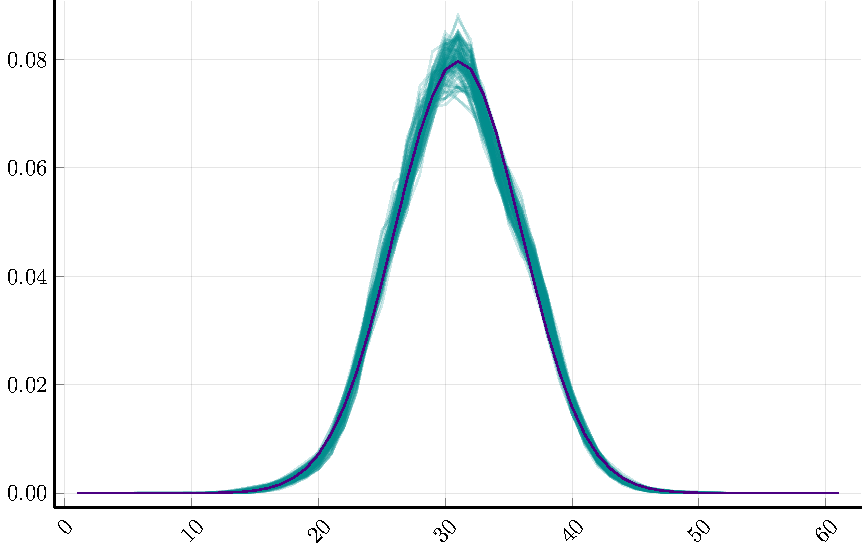
\includegraphics[width=\linewidth]{Figures/1a/W.pdf}
		\caption{Case 1a - Normal(0,1), N=3000} 
	\end{subfigure}
	\begin{subfigure}[t]{.4\textwidth}
		\centering
		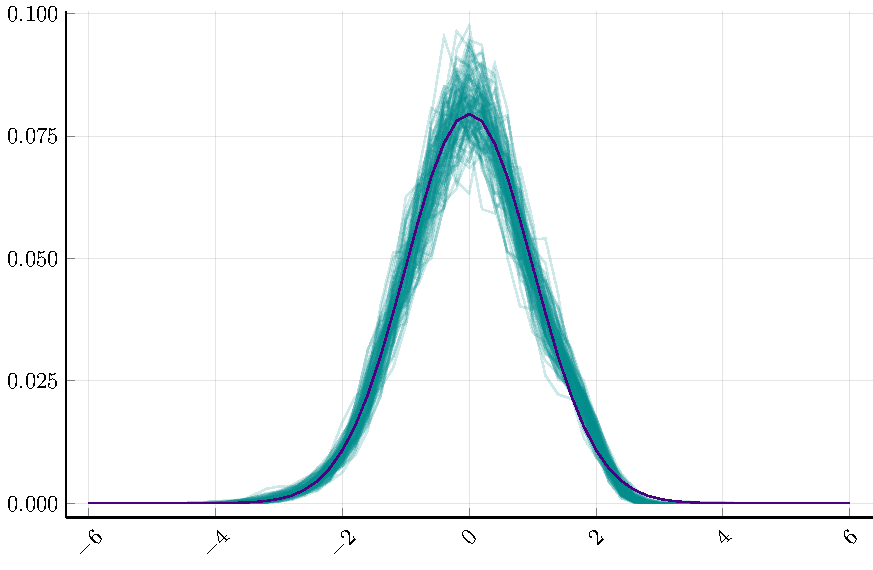
\includegraphics[width=\linewidth]{Figures/1b/W.pdf}
		\caption{Case 1b - Normal(0,1), N=600} 
	\end{subfigure}
	\vspace{20px}
	\begin{subfigure}[t]{.4\textwidth}
		\centering
		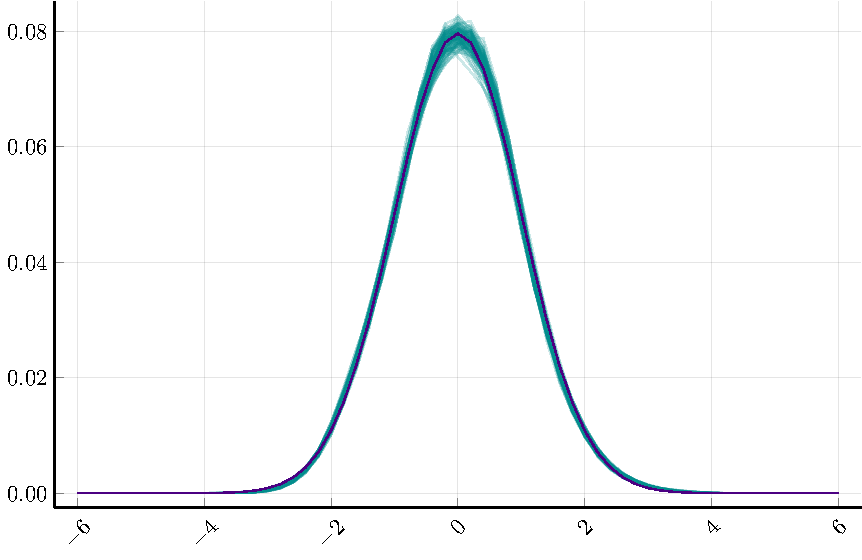
\includegraphics[width=\linewidth]{Figures/1c/W.pdf}
		\caption{Case 1c - Normal(0,1), N=6000} 
	\end{subfigure}
	\begin{subfigure}[t]{.4\textwidth}
		\centering
		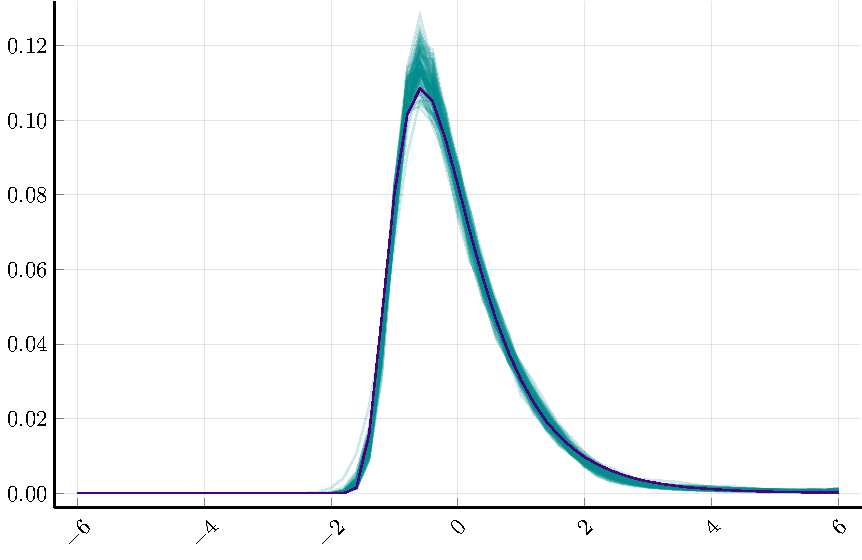
\includegraphics[width=\linewidth]{Figures/2a/W.pdf}
		\caption{Case 2a - LogNormal(0,0.5), N=3000} 
	\end{subfigure}
	\vspace{20px}
	\begin{subfigure}[t]{.4\textwidth}
		\centering
		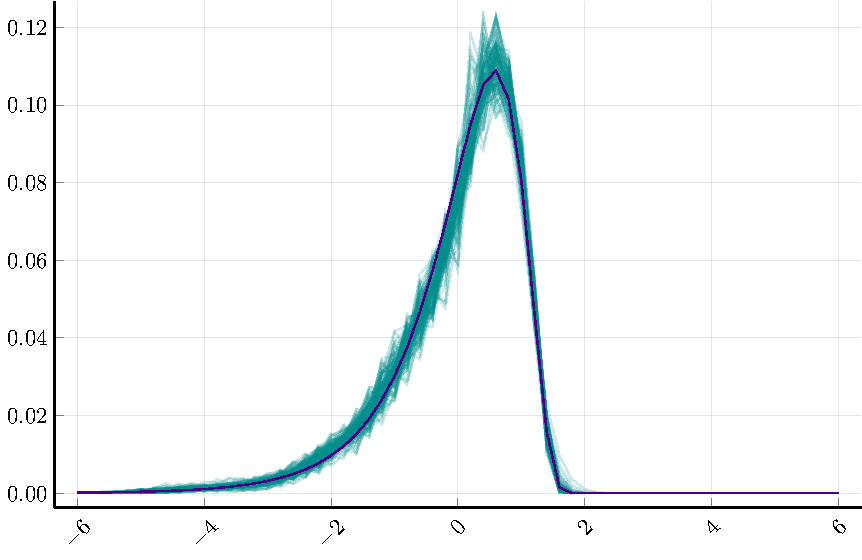
\includegraphics[width=\linewidth]{Figures/2b/W.pdf}
		\caption{Case 2b - flipped LogNormal(0,0.5), N=3000} 
	\end{subfigure}
	\begin{subfigure}[t]{.4\textwidth}
		\centering
		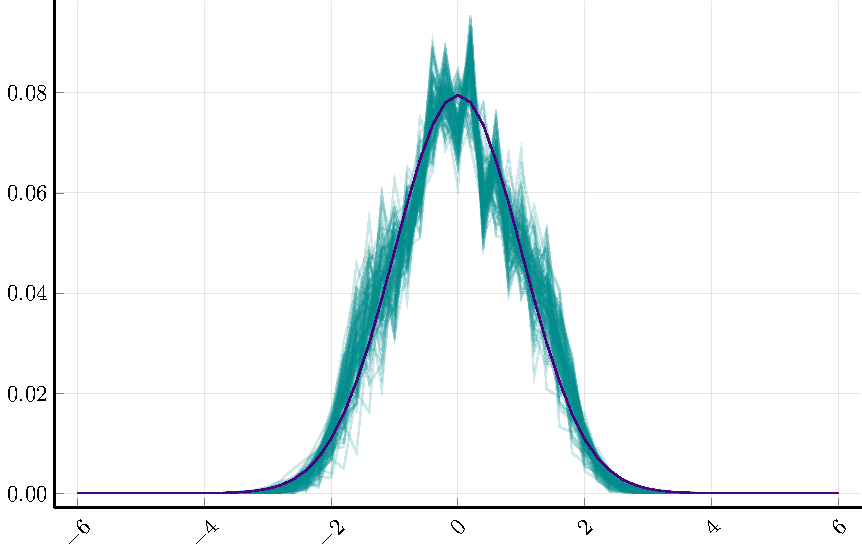
\includegraphics[width=\linewidth]{Figures/3/W.pdf}
		\caption{Case 3 - Normal(0,1), N=3000} 
		\centering
	\end{subfigure}
	\vspace{20px}
	\begin{subfigure}[t]{.4\textwidth}
		\centering
		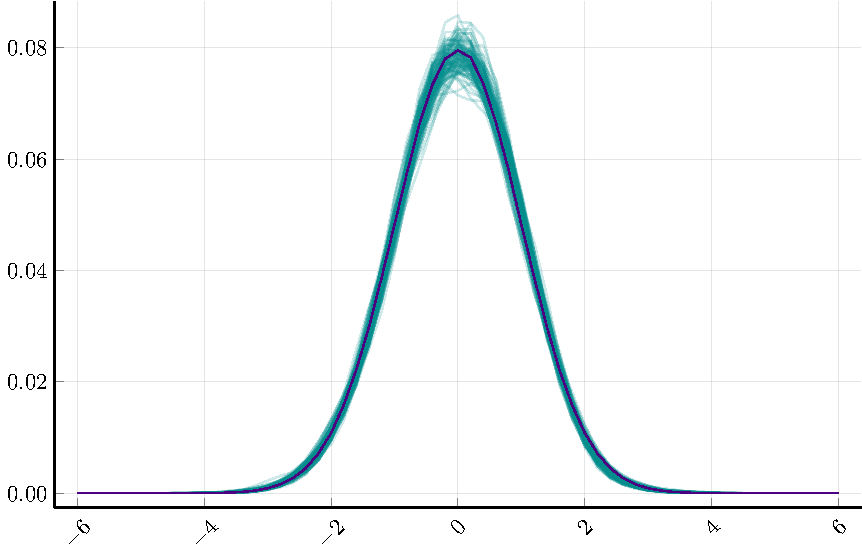
\includegraphics[width=\linewidth]{Figures/4/W.pdf}
		\caption{Case 4 - Normal(0,1), N=3000} 
		
	\end{subfigure}
	%\textbf{Distribution of RMSEs of estimates across items and test-takers }\par\medskip
	\caption{Retrieval of the latent probability distribution by cubic-spline}
	\label{fig:cubicspline}
\end{figure}


\subsubsection{Computational performance}


To compare the performance of the three considered algorithms, we evaluate their CPU times, and the iteration counts averaged across the $S$ simulations. The results for the cases under analysis are summarized in the following table.

\begin{table}[H]
	\label{tab:cases}
	\renewcommand{\arraystretch}{1.5}%
	\centering
	\caption{Computational power summary}
	\begin{tabular}{ l  c c  c  c c c  }
		\toprule
		& \multicolumn{3}{c}{average CPU time} & \multicolumn{3}{c}{average iterations count} \\
		\toprule
		& {jl} &{mirt} & {mirt\tiny{EHW}} & {jl} &{mirt} & {mirt\tiny{EHW}}  \\
		\midrule
		1a    &\textbf{5.75} & 11.90 &17.27 &88.88 & 55.12  & 59.99  \\%[5pt]
		1b    &\textbf{2.55}  & 9.137 &16.75 & 109.54  &51.31 & 69.12 \\%[2pt]
		1c    &\textbf{10.58}  &14.69  & 20.50 & 92.73 &56.42 & 59.31\\%[2pt]
		2a    & \textbf{7.75}  &12.32 & 21.39 &105.85  & 47.09 & 65.43 \\%[5pt]
		2b    &\textbf{5.77}  & 9.47 & 97.42 & 97.35 & 49.87 & 169.73\\%[5pt]
		3    & \textbf{12.81} & 24.81 &37.54 & 222.28  & 140.44 & 151.14\\%[5pt]
		4    & \textbf{3.59} & 12.98  &16.45  &58.17  &43.86  &53.61 \\%[5pt]
		\bottomrule   
		
	\end{tabular}
	
\end{table}

As it is clearly noticeable, \texttt{Julia} has a better time performance in all the studied cases. However, more iterations than \texttt{mirt} are needed to reach convergence of the estimations. We believe that the latter phenomenon is due to acceleration techniques applied in the \texttt{R} package, such as Ramsay or SQUAREM \parencite{varadhan2008simple}. In our approach no acceleration has been implemented to avoid instability in the first iterations where the rescale of the latent distribution and the cubic-spline interpolation is performed. 
Moreover, we think that our code is further optimizable by introducing more parallel or distributed computing \texttt{Julia} tools\footnote{See \url{https://docs.julialang.org/en/v1/manual/parallel-computing/index.html}}.

\subsubsection{Sampling distribution of IRT item parameters}

The following plots show the sampling distributions of the IRT parameters, $\hat{a}$ and $\hat{b}$, of the first 10 items of the pool obtained by performing the non-parametric and parametric bootstrap described before. The results are reported only for the \emph{standard setup} (case 1a).
As can be seen, there is not any discernible difference between the results of the two approaches. In both cases, the true value of the item parameter (black dot) is not always between the first and third quartiles of the distribution. At least, the simulated value it is never in the outlier area, that is the area outside the whiskers which delimit the interval obtained by multiplying by 1.5 the range between the first and third quartile.

\captionsetup[subfigure]{labelformat=empty}

\begin{figure}[H]
	\centering
	\begin{subfigure}[t]{0.8\textwidth}
		\centering
		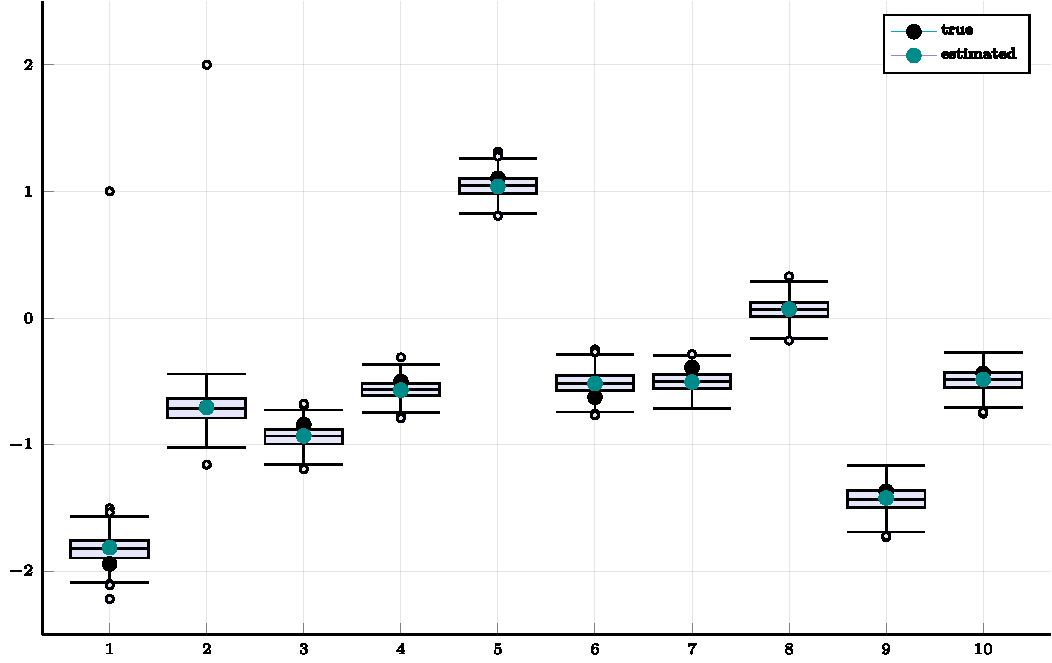
\includegraphics[width=\linewidth]{Figures/bootstrap/BSb_npar.pdf}
		\caption{(1) Easiness parameter $b$} 
	\end{subfigure}
	\begin{subfigure}[t]{0.8\textwidth}
		\centering
		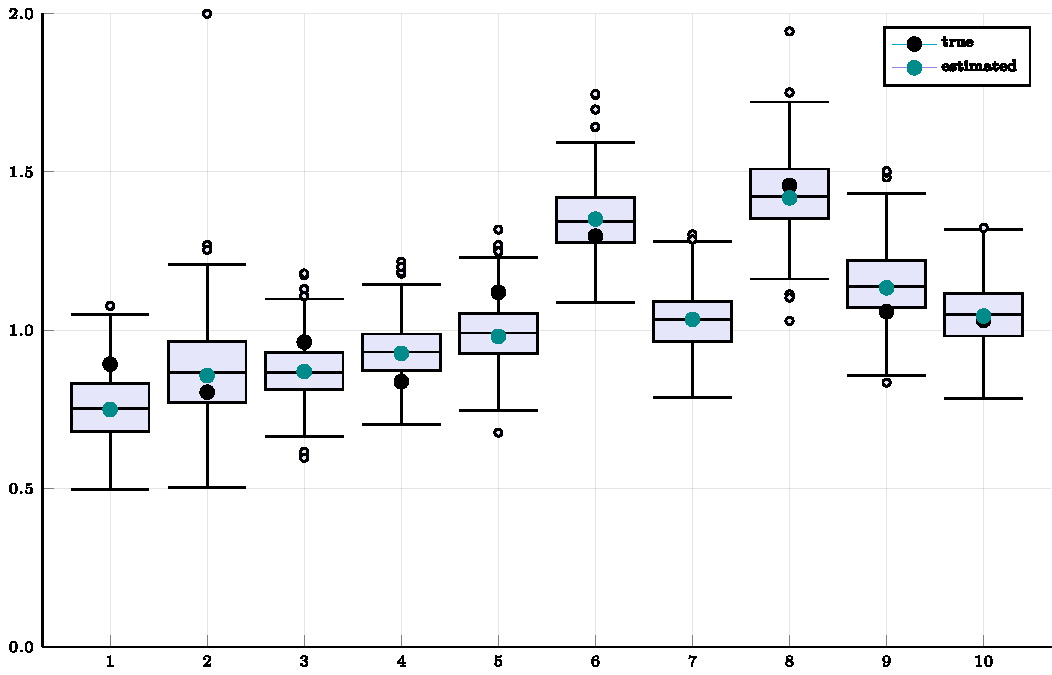
\includegraphics[width=\linewidth]{Figures/bootstrap/BSa_npar.pdf}
		\caption{(2)  Discrimination parameter $a$} 
	\end{subfigure}
	
	%\textbf{Distribution of RMSEs of estimates across items and test-takers }\par\medskip
	\caption{Case 1a - Non-parametric bootstrap - Sampling distributions of first 10 item parameters.}
	\label{fig:sampdist10npar}
\end{figure}

\captionsetup[subfigure]{labelformat=empty}

\begin{figure}[H]
	\centering
	\begin{subfigure}[t]{0.8\textwidth}
		\centering
		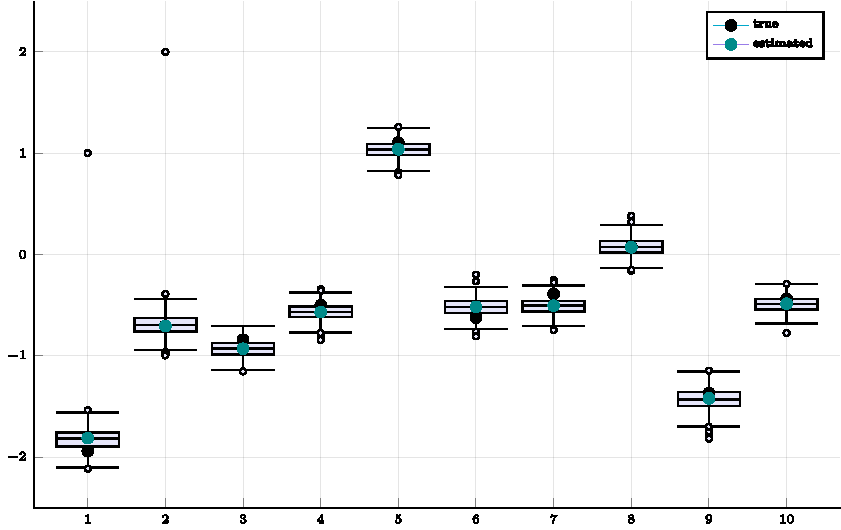
\includegraphics[width=\linewidth]{Figures/bootstrap/BSb_par.pdf}
		\caption{(1) Easiness parameter $b$} 
	\end{subfigure}
	\begin{subfigure}[t]{0.8\textwidth}
		\centering
		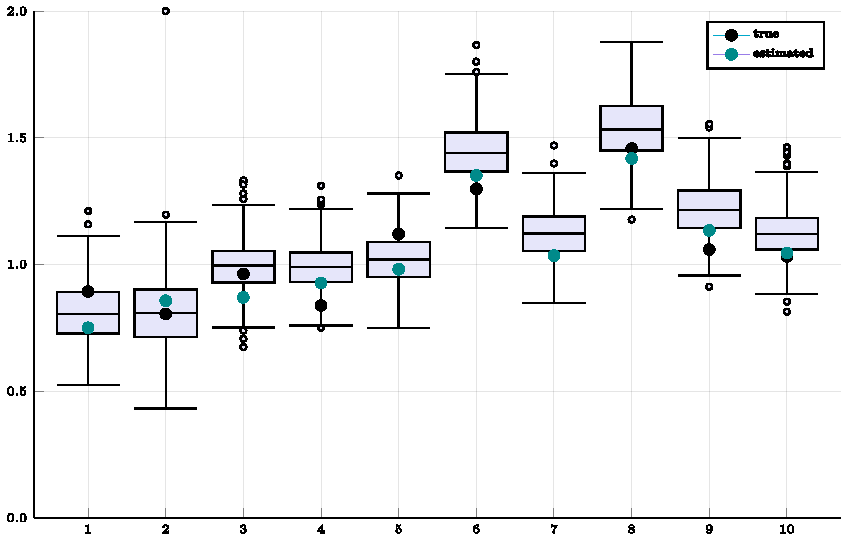
\includegraphics[width=\linewidth]{Figures/bootstrap/BSa_par.pdf}
		\caption{(2) Discrimination parameter $a$} 
	\end{subfigure}
	
	%\textbf{Distribution of RMSEs of estimates across items and test-takers }\par\medskip
	\caption{Case 1a - Parametric bootstrap - Sampling distributions of first 10 item parameters}
	\label{fig:sampdist10par}
\end{figure}

	% Chapter 3

\chapter{Chance-constrained test assembly}
\label{sec:CC}

The test information function (TIF) is a key object both in the IRT and in the test assembly framework. Most of the automated test assembly models (ATA) are} based on this quantity that usually appears in the objective function, being the goal for the optimization model. As explained in Section~\ref{ch:ATA} the IIFs are considered as given values. This approach may lead to several issues such as infeasibility of the MINIMAX or MAXIMIN model, e.g. if it is not possible to find $T$ parallel tests that have TIFs inside a fixed interval around the targets. Another issue is the incorrect interpretation of the assembly results. For example, if the calibration algorithm had produced wrong estimates for the item parameters and hence the item information functions are not accurate enough, the TIF of the assembled test might be overestimated. Regarding the latter issue, a good test assembly model would consider the variation of the item parameter estimates in order to build test forms in a conservative fashion, i.e., it would produce tests with a maximum plausible lower bound of the TIF.  

There is a need for better treatment of this problem in test assembly models. My attempt in this dissertation is to incorporate uncertainty in the optimization models most seen in practice and in literature for simoultaneous multiple test assembly using the modern techniques of the stochastic programming framework. Chance-constraints (or probabilistic constraints) are a natural solution to the mentioned problems. They are among the first extentions proposed in the stochastic programming framework to deal with constraints where some of the coefficients are uncertain \parencite{charnes1963deterministic,krokhmal2002portfolio}. In particular, by adjusting a conservative parameter $\alpha$, also called \emph{risk level}, it is possible to modulate the level of fulfilment of some probabilized constraints enabling the user to relax or to tighten the feasibility of the problem. Narrowing our focus on the MAXIMIN test assembly model introduced in \ref{sec:ata}, a percentile optimization model would maximize a reasonable lower bound of the TIF, its $\alpha$-quantile, approximated by the $\lceil \alpha R \rceil$-th ranked value of the TIF computed on the $R$ bootstrap replications of the estimates of item parameters.
%In case of infeasibility another approach would be relax some constraints by randomizing their fulfillment.

An introduction to the idea of chance-constrained modeling is provided in the first Section together with a brief literature review of the issues and of the existing methods to solve this type of problems. Subsequently, a chance-constrained version of the MAXIMIN test assembly model is proposed and, since this novel model cannot be approximated by a linear formulation, a heuristic based on simulated annealing \parencite{goffe1996simann} has been developed. This technique can handle large-scale models and non-linear functions. A Lagrangian relaxation formulation helps to find the most feasible/optimal solution and, thanks to a random variable, more than one neighborhood of the space is explored avoiding to being trapped in a local optimum. Moreover, the proposed heuristic can solve a wide class of optimization problems characterized by having binary optimization variables and a separable objective function. Furthermore, the details of the results of the retrieval of the empirical distribution function of the TIF are provided in Section \ref{sec:edfTIF}.

Several simulations of ATA problems are performed and the solutions are compared to CPLEX 12.8.0 Optimizer, a benchmark solver in the linear programming field. In particular, since our heuristic is able also to solve the classical ATA models we compare the results of the optimization in both the framework: exact and chance-constrained. Every described algorithm is coded in the open-source framework Julia. A package written in Julia has been released \footnote{\url{http:\\github.com\\giadasp\\CCATA}, available in private version, ask to \url{giada.spaccapanico2@unibo.it} for the credentials.}.

\section{Chance-constrained modeling}

In the past five decades, the developments in the theory of choice under risk in financial applications, e.g. portfolio optimization where the prices of instruments are random variables (see \textcite{rockafellar2000optimization,rockafellar2001uryasev}),  followed the expected mean-variance approach \parencite{chen1973quadratic,freund1956introduction,scott1972practical}). In risk management and reliability applications the decision maker must select a combination of assets for building a portfolio by maximizing their utility function. The latter is defined in terms of the expected mean and variance of the returns or of the prices of the instruments which are uncertain coefficients in the linear objective or constraints of the optimization model. More recently, instead, the regulations for finance businesses require to reformulate the problem in terms of percentiles of loss distributions. These requirements gave rise to the theory of \emph{chance-constraints}, also called probabilistic constraints, originally proposed by \textcite{Charnes1959}. 

The probabilistic constraints present coefficients which are assumed to be randomly distributed and they are subject to some predetermined threshold $\alpha$ of the constraints fulfilment. Modifying $\alpha$ it is possible to relax or tighten some constraints modulating the level of conservativeness of the model.
The standard form of a mixed-integer optimization problem can be represented by  

		\begin{alignat}{4}\label{eq:optModel2}	\underset{\mathbf{x}}{\arg \min} \quad & f(\mathbf{x}) &&\quad  & \\
	\nonumber
	\text{subject to} \quad & g_j(\mathbf{x}) \leq 0 &&\quad & j=1,\ldots,J
	\end{alignat}
	\begin{equation}\nonumber
		 \mathbf{x} \in \mathbb{Z}^p \times \mathbb{R}^{n-p}   
	\end{equation}

where $f(\cdot)$ is the objective function to be optimized, $\mathbf{x}$ is the vector of $p$ integer and $n-p$ continuous optimization variables. Both $f(\cdot)$ and $g(\cdot)$ are scalar functions.\\
The optimization domain is $D=\text{dom}(f) \cap \bigcap_{j=1}^J \text{dom}(g_j)$ and the set \\ $\mathbf{X}=\left\{\mathbf{x} : \mathbf{x} \in D, g_j(\mathbf{x}) \leq 0 \ \forall j \right\}$ is called \emph{feasible set}, i.e. a solution $\mathbf{x}$ is feasible if it is in the optimization domain and satisfies the constraints. Starting from \eqref{eq:optModel2}, a chance-constraints reformulation will add the following set of constraints:

\begin{equation}\label{eq:CCcon}
\mathbb{P}\left[g_k(\mathbf{x},\boldsymbol{\xi})\leq 0\right] \geq 1-\alpha \quad k=1,\ldots,K
\end{equation}

where $\boldsymbol{\xi}$ is a vector of random variables. This formulation seeks a decision vector $\mathbf{x}$  that minimizes the function $f(\mathbf{x})$ while satisfying the chance constraints $g_k(\mathbf{x},\boldsymbol{\xi})\leq 0$ with probability at least $1-\alpha$. Such constraints imply having a function to compute (or better approximate) the probability and a solver which can deal with that function. Whenever a MAXIMIN principle is applied, they can be seen as \emph{percentile optimization} problems \parencite{krokhmal2002portfolio} because the probability in \eqref{eq:CCcon} is replaced by the $\alpha$-th percentile of the distribution function of $g_k(\mathbf{x},\boldsymbol{\xi})$ and these percentiles must be maximized.

Despite the old age, chance-constrained models are, still hard to be solved. An issue is the general non-convexity of the probabilistic constraints. Even if the original deterministic constraints\footnote{$g_k(\mathbf{x},\boldsymbol{\xi})$ where $\boldsymbol{\xi}$ is not random.} were convex the respective chance-constraints may be non-convex. In general they are usually untractable (see \textcite{Nemirovski}) because even if they are convex the quantiles of the random variables are difficult or impossible to compute. Examples of approximations of chance-constraints are the linearization method called sample average approximation \parencite{Ahmed2008} and the case when the random variables follow a known multivariate distribution with known mean and variance. For the first case, a big-M approach is needed to deal with the indicator function bringing numerical instability in the optimization. The second approach instead imposes strong distributional assumptions (see \textcite{Kataria} for a list of distributional assumptions) and, since they are based on the Chebishev inequality they require a modest number of elements in the summations to achieve the convergence, they need also a solver which can deal with second-order conic constraints, the most difficult type of convex functions to be optimized. All the mentioned formulations increase exponentially the number of optimization variables, thus they are not suitable for large-scaled models.

Other approaches rely on discretization of the random variable and hence the model is optimized in all possible scenarios (i.e. realizations of the random variables) thus they do not fit to problems with a large number of random variables because all the patterns must be considered \parencite{margellos2014road,wang2011chance,tarim2006}. In finance, such models are called VaR (value at risk) and they are usually characterized by non-concavity and hence computational intractability except in certain cases where returns are known to have an elliptical distribution, see for example \textcite{vehvi2003} or \textcite{mcneil2005}. 

Another question is the domain of optimization. Usually, stochastic optimization models are addressed in the case of continuous optimization variables while mixed-integer problems are still neglected because of their greater complexity. Given a lack in optimization techniques which can handle such problems, we first use a Monte-Carlo approach to approximate the quantiles in a percentile optimization perspective and, in Section \ref{sec:heur}, we propose an heuristic to solve the chance-constrained test assembly model defined previously. In the last Section a simulation study is conducted to show the practical and computational advantage of our approach in the test assembly research field.

\section{Chance-constrained test assembly model}\label{sec:CCATA}

In the context of test assembly the optimization models used for selecting the items does not consider the inaccuracy of the estimates of item parameters \parencite{VDL2005}. However, estimates are never exact. Thus, ignoring the potential imprecision can lead to wrong conclusions and misinterpretations of the results such as overestimation of the information function and hence of the accuracy of the test in ability estimation. Some attempts to include uncertainty in the test assembly models have been done by \textcite{veldkamp2013application} and \textcite{veldkamp2013uncertainties} who developed and applied the robust model introduced in \textcite{bertsimas2003robust}. The mentioned automated test assembly model considers the standard error of the estimates and a protection level $\Gamma$ that indicates how many items in the model are assumed to be changed in order to affect the solution. It treats the uncertainty in a deterministic way and, given $\Gamma$, it adjust the solution adopting the most conservative approach, because standard errors are the maximum expression of uncertainty of the estimates.

In contrast, if we consider the MAXIMIN model \eqref{eq:maximinmodel} its chance-constrained equivalent would replace the constraints \eqref{eq:MMAXIMIN2} involved in the maximization of the TIF by 

\begin{equation}\label{eq:CCATA}
\mathbb{P}\left[\sum_{i=1}^I I_i(\theta_{k_t}) x_{it} \ge y \right] \geq 1-\alpha , \ \forall t,k_t,
\end{equation}

where $t=1,\ldots,T$ are the test to be assembled and $\theta_{k_t}$ are the ability points in which the TIF of the test $t$ must be maximized. We decided to ignore the weights to simplify the notation but the extension to the weighted case is straightforward. We will call the model \eqref{eq:CCATA} \emph{chance-constrained MAXIMIN}, or CCMAXIMIN. The key element of this model is, again, the information function which is assumed to be random. This assumption arises, as already explained, by the necessity of taking into account the uncertainty of the item parameter estimates, of which the item information function is a statistic (see \eqref{eq:infofun2pl} for an example).

The CCMAXIMIN model allows to maximize the expected precision of the assembled tests in estimating the latent trait of the test-takers at pre-determined ability points with a high  confidence level if the $\alpha$ is chosen to be next to zero. In terms of probability we can say that the constraints in \eqref{eq:MMAXIMIN2} must be fulfilled with a probability at least $1-\alpha$. Adjusting the confidence level it is possible to relax or tighten the fulfilment of the chance-constraints setting a specific conservative attitude, i.e. a small $\alpha$ means an high level of conservatism, on the contrary a big $\alpha$ means an almost relaxation of the constraints. This is the novelty of the CCMAXIMIN model with respect to the robust model proposed in \textcite{veldkamp2013application,veldkamp2013uncertainties} which, instead, perform a worst-case optimization. 

Once the chance-constraints have been defined, a way to evaluate the probability in \eqref{eq:CCATA} must be found in order to quantify the feasibility of a solution. To solve this problem, some methods rely on assumptions on the probability distribution of $\boldsymbol{\xi}$, such as the multivariate normal \parencite{kim1990deterministic}. Others try to approximate the probability using samples of the random variable obtained by a Monte Carlo simulation \parencite{Ahmed2008} which is a specific case of a scenario generation where all the scenarios have the same probability of occurrence. 
We decided to use the Monte Carlo method because of its flexibility and adaptability to our problem. 

In particular, our random variable is the TIF of a test form, that  is a statistic on some estimates which are uncertain. There are different ways to sample from the distribution function of this random variable: given the standard errors of the estimates, the samples can be uniformily drawn from their confidence intervals\footnote{as in the robust model \parencite{veldkamp2013application}}; otherwise, if a Bayesian estimation is carried on, the last samples in the Markov chain can be used. In this dissertation the samples are picked by bootstrapping the estimation process and the empirical distribution function of the statistic is obtained. The bootstrap \parencite{efron1993} is a very powerful algorithm to extract information about the distribution of some estimate, provided that the method of resampling is accurate enough to reproduce the underlying data generation process. The details of the retrieval of the empirical distribution function of the TIF are reported in the following section.

\subsection{Empirical measure of the TIF}\label{sec:edfTIF}

Conventionally, the estimates of IRT item parameters are considered as known values in test assembly models \parencite{VDL2005}. Test assembly models ignore the uncertainty related to the calibrated items and thus they often yield an overstated measurement accuracy of the assembled tests in terms of their TIFs.
A standard approach to extract the uncertainty related to the estimates of the item parameters would be first, sampling a high number of plausible values of the item parameters $\boldsymbol{\xi}_i$ in the confidence intervals built using the standard errors of the estimates and, secondly, computing the related IIFs at target $\theta$ points. This may be an optimal starting point to assemble robust tests, \parencite[see]{veldkamp2013uncertainties, veldkamp2013application} but it has its own downsides because a uniform interval of plausible values is assumed. Another attempt to account for the influence of sampling error in the Bayesian framework has been made by \textcite{Yang2012} who proposed a multiple-imputation approach with the aim to better measure the latent variable of a respondent. 

In \textcite{matteucci2012prior} it has been shown that the behavior of the estimates of item parameters usually follows joint densities not equal to the product of their marginals, suggesting the presence of an underlying dependence structure. This observation motivated the search for a new technique to recreate the distribution function of the IIFs and hence iof the TIF. Our solution is based on bootstrapping the calibration process (see \textcite{efron1993} for a gentle introduction to the bootstrap), in particular, the observed vectors of responses (one vector for each test-taker) are resampled with replacement $R$ times and the item parameters are re-estimated for each sample. In this way, it is possible to preserve the natural relationship between the items and, given the ability targets, it is possible to compute their IIFs. After that, given a set of items, we can build a test form and compute its TIF for each of the $R$ replications. The resulting sample constitutes the \emph{empirical distribution function} of the TIF. 

More formally, let $\boldsymbol{\xi}_1, \ldots, \boldsymbol{\xi}_R$ be an independent identically distributed (iid) sample of $R$ realizations of a $I$-dimensional random vector $\boldsymbol{\xi}$, its respective empirical measure is 
$$\hat{F}_R : = R^{-1} \sum_{r=1}^R \Delta\boldsymbol{\xi}_r,$$
 where $\Delta\boldsymbol{\xi}_r$ denotes the mass at point $\boldsymbol{\xi}_r$\footnote{$\Delta\boldsymbol{\xi}_r(A)=1$ when $\boldsymbol{\xi}_r\in A$}. Hence $\hat{F}_R$ is a discrete measure assigning probability $1/R$ to each sample. In this way we can approximate the probability in the left-hand side of \eqref{eq:CCcon} by replacing the true cumulative distribution function of $\boldsymbol{\xi}$ by $\hat{F}_R$. 
 Let $\mathbf{1}_{(-\infty, 0]}\{x\} :\mathbb{R} \rightarrow \mathbb{R}$ be the indicator function of $x$ in the interval $(-\infty, 0]$, i.e.,
 

 	$$\mathbf{1}_{(-\infty, 0]}\{x\}= 
 	\begin{cases} 
 	0, & \mbox{if } x\mbox{ $> 0$} \\
 	1, & \mbox{if } x\mbox{ $\leq 0$},
 	\end{cases}
$$

Thus, given a specific chance-constraint $k$, a known set of optimization variables $\mathbf{x}$ and a sample $\boldsymbol{\xi}_1, \ldots, \boldsymbol{\xi}_R$ of our random vector, we can rewrite
\begin{alignat}{2}
\mathbb{P}\left[g_k(\mathbf{x},\boldsymbol{\xi})\leq 0\right] = &  \mathbb{E}_{F}\left[\mathbf{1}_{(-\infty, 0]}\{g_k(\mathbf{x},\boldsymbol{\xi})\} \right]\\
\approx & \mathbb{E}_{\hat{F}_R}\left[\mathbf{1}_{(-\infty, 0]}\{g_k(\mathbf{x},\boldsymbol{\xi})\} \right] \\
= & \frac{1}{R} \sum_{r=1}^R \mathbf{1}_{(-\infty, 0]}\{ g_k(\mathbf{x},\boldsymbol{\xi}_r) \}.
\end{alignat}

That is, the chance-constraint is evaluated by the proportion of realizations with $g_k(\mathbf{x},\boldsymbol{\xi}) \leq 0$ in the iid sample.

Adopting the same principle to the left-hand side of the chance-constraints in \eqref{eq:CCATA}, the CCMAXIMIN model can be approximated by:
\begin{alignat}{4}\label{eq:CCMAXIMINapprox}
\underset{\mathbf{x}}{\arg \min} \quad & -y &&\quad  & \\
\nonumber
\text{subject to} \quad &\frac{1}{R}\sum_{r=1}^R\mathbf{1}_{[y,\infty)}\{ \mathbf{I}_r(\theta_{k_t})'\mathbf{x}_t \} \geq 1-\alpha ,  &&\quad & \forall t,k_t,\\\nonumber
& g_j(\mathbf{x}_t) \leq 0 &&\quad & \forall j,t,
\end{alignat}
\begin{equation}\nonumber
\mathbf{x}_t \in \{0,1\}^I, y \in \mathbb{R}^+,
\end{equation}
where $\mathbf{I}_{r}(\theta_{k_t})$ is the vector of the $I$ item information functions at pre-defined $\theta_{k_t}$ points computed from the estimates of the item parameters in the $r$-th bootstrap replication. 

The model \eqref{eq:CCMAXIMINapprox} is clearly non-convex because of the chance-constraints (see, \textcite{rockafellar2000optimization,rockafellar2001uryasev} for the demonstration) and most of the commercial solver doesn't deal with indicator functions, to overcome this issues we solved the previous model by an heuristic described in the next Section.

To have an idea of the empirical distribution function of the information function of an item with true values of discrimination and easiness parameters, $a=1$ and $b=0$, estimated by bootstrapping the calibration of a 2-parameter logistic model following the algorithm described in \ref{sec:Julia}, the histograms for several values of the latent trait are reported herewith:

%\includegraphics[keyvals]{imagefile} 3x3 theta= [-2.0,-1.5,-1.0,-0.5, 0.0, 0.5, 1.0, 1.5, 2.0]
 


\color{black}
\subsection{Solving the CCMAXIMIN model}

Since the model \eqref{eq:CCMAXIMINapprox} is not practically solvable by commercial solvers, we devoloped a heuristic based on the \emph{simulated annealing} approach.
It is a flexible and simple numerical procedure that can be used to find an optimal solution for a model of arbitrary complexity which seeks the minimal of a function, $f(\mathbf{x})$, called \emph{loss}. The loss function serves as a distilled form of the greater problem and it depends on the values of some fixed coefficients and optimization variables $\mathbf{x}$, a vector $d$ dimensional. Changing the value of the objective variables the returned loss function will increase, decrease or remain constant telling if the variation is useful or not to reach a minimum (preferrably global). Once the loss function is determined and it is evaluable for each value of the optimization variables the simulated annealing algorithm can be applied leading to the best configuration of $\mathbf{x}$ which minimizes the loss. In practice, an inital value of $\mathbf{x}$, namely $\mathbf{x}_0$, is chosen and a forward pass to evaluate $f(\mathbf{x}_0)$ is performed. At each successive step, $s>0$, the current $\mathbf{x}_s$ is a perturbation of $\mathbf{x}_{s-1}$ in the sense that one of more elements are changed in order to explore another neighbourhood of the solution space.

The movement from a neighbourhood to another will be called \emph{journey} and how it is performed depends on the problem under inspection and on how far we want to travel from the last accepted solution, called incumbent. If the loss for the perturbed $\mathbf{x}_s$ is more or equally optimal than the previous, then $\mathbf{x}_s$ is accepted as a basis for the next iterations. However, if the solution is less optimal (e.g. the loss increase), the choice of whether discard or keep it depends on the value of a sample of a random variable. The random variable is built considering the amount of variation of the loss function induced by the journey and the state of the cooling schedule defined by the temperature $T(s)$ deterministically determined. Here the Metropolis Hastings algorithm appears and plays an important role in defining the convergence properties of the heuristic. The details are provided in the next paragraph.

\subsubsection{Simulated Annealing}

The principle of cooling schedule comes from the language used to describe mechanical processes of metal annealing, which involves heating a metallic object to a very high temperature and gradually cooling it. By letting the metal cool down, the particles (the optimization variables) arrange themselves into the lowest possible energy state (evaluated loss function). The atoms are allowed to move to further areas of the space (neighbourhoods) at hot temperatures than at low temperatures, this avoid to be stuck in local minima in the first phases of the annealing. After the minimum temperature has been reached a reannealing can be performed to explore other areas of the space. This allows to have an arbitrary number of non-unique solutions to compare and select. The system temperature, $T(s)$, is a non-increasing function with respect to the iteration count. It has been proved that, if an infinite number of iterations is made, the algorithm will reach the global minimum \parencite{belisle1992}. Since the infinite assumption cannot be fulfilled in practice, a reasonable number of iterations is chosen, usually depending on the maximum allowed computational time.

The random variable which rules the acceptance/rejection step comes from the normalized Boltzmann factor

\begin{equation}
\mathbb{P}\left[E\right]=\frac{1}{z(T)}e^{\frac{-E}{kT}}
\end{equation} 

which determines the probability of observing a particular energy $E$ given a termperature $T$, a normalizing factor $z(T)$ and a Boltzmann constant $k$. In practice, if at the iteration $s$ we observe $f(\mathbf{x}_s)$ and this is higher than $f(\mathbf{x}_{s-1})$ the probability of keeping $\mathbf{x}_s$ is equal to the probability of the variation, $\Delta f_s$, in the loss function:
\begin{equation}\label{eq:boltz}
\mathbb{P}\left[\Delta f_s\right]=\frac{e^{\frac{-f(\mathbf{x}_s)}{kT(s)}}}{e^{\frac{-f(\mathbf{x}_{s-1})}{kT(s)}}}= e^{\frac{-\Delta f(\mathbf{x}_s)}{kT(s)}}.
\end{equation}
If the variation in energy is large the probability that the parameters will be kept is low, while for a small variation they might be accepted. In this way, the algorithm allows to escape from local minima, increasing the chance that the global minimum will be found. The actual choice is made by comparing the value given in \eqref{eq:boltz} to a random variate from the uniform distribution. If the random value is smaller, the parameters are kept. As time goes on and the system temperature drops, however, the probability of keeping the state approaches zero, even for small changes in energy.

\subsubsection{Heuristic}\label{sec:heur}

Adopting the simulated annealing algorithm it is possible to solve all the test assembly models which take the form \eqref{eq:LRsingClassTest}. The heuristic we developed is inspired by the work of \textcite{Stocking1993} because the constraints in the optimization model are treated as part of the loss function using the hinge function and more in general, through the Lagrange relaxation, two main concepts introduced in \ref{sec:lagrange}. 
The algorithm is based on the separation of the problem, in particular we differentiate the $T$ vectors $\mathbf{x}_1, \ldots, \mathbf{x}_T$ of $I$ binary variables, each vector $\mathbf{x}_t$ corresponds to a test assembly sub-problem for the test form $t$. Also the $T$ matrices and vectors involved in the linear constraints and in the objective function are kept separated. Along the iterations each of the test is evaluated separatedly in terms of optimality and feasibility. This separation allows to speed up the algorithm since all the algebraic operations are made on smaller objects. The only constraints which are not separable are the overlap \ref{sec:test-overlap} and the item use \ref{sec:item-use} which are evaluated on the full-length vector of optimization variables.

The simulated annealing has the disadvantage that is hardly able to find the feasible space of a problem, this is why we decided to start our heuristic by a \emph{fill up} sequential phase in which the worst performing test, both in terms of optimality and feasibility\footnote{In practice we allow the user to decide if the fill up phase must be done by considering only the feasibility of the problem or adding the optimality evaluation.}, is "filled up" with the best item available in the item pool. After the item has been assigned, the process is repeated until all the tests have reached their maximum length, i.e. they are all "filled-up".

Once the first step is performed, luckily we have at least a feasible solution to process with the simulated annealing principle. In details, the first $W$ worst tests $\mathbf{x}_1,\ldots,\mathbf{x}_W$ are taken and a fixed number of items $V$, already taken in these tests, is sampled, namely $\mathbf{x}_{1,1},\ldots,\mathbf{x}_{1,V}, \ldots, \mathbf{x}_{W,1}, \ldots, \mathbf{x}_{W,V} $. These sampled items are first, removed and secondly, switched with all the other available items in the pool. The test resulting from the removal and the switch is accepted with a chance equal to \eqref{eq:boltz}. After the sampling phase, the performance of the tests is again evaluated and if the termination criteria have not been met, tests and items are sampled again. When a certain convergence in the objective is attained we say that a neighbourhood of the space has been explored. The user can decide how far he/she wants to go from the most recent solution and hence how many neighbourhoods he/she wants to explore. If the \emph{journey} is not completed, the last solution is substantially perturbed and the heuristic performs again the \emph{fill up} and sampling steps. 

The result of the heuristic is a set of solution of length $H$ which is the number of neighbourhoods explored. It is also possible to decide how many of these areas must be evaluated just in terms of feasibility, $H_f$, and how many in terms of optimality, $H_o$, i.e. $H=H_f+H_o$. In this way the test assembler has a wider choice of optimally assembled tests in terms of other features not considered in the assembly model, such as content validity.

The hyperparameters (i.e. parameters chosen by the user) in the algorithms are several, the following list summarize all the customizable features:
\begin{itemize}
	\item \textbf{Lagrange relaxation:} 
	\begin{itemize}
		\item $\beta \in  [0,1]$, as in \eqref{eq:LRsingClassTest}, it serves as a balancing between optimality and feasibility. A $\beta$ approaching one puts more emphasis on the optimality of the solution. Viceversa an almost zero $\beta$ takes into account only the feasibility of the solution.
		\end{itemize}
	\item \textbf{simulated annealing:}\begin{itemize}
		\item $F_f$: number of feasible \emph{fill-up} phases;
		\item $t_0$: starting temperature;
		\item \texttt{geom\_temp}: the factor by which the temperature is geometrically decreased at each iteration $s$, i.e. $t_s=t_{s-1}/\text{\texttt{geom\_temp}}$;
		\item $W$: number of worst performing tests to sample;
		\item $V$: number of already selected items in each of the $W$ tests to sample.
	\end{itemize}
	\item \textbf{termination criteria:} \begin{itemize}
		\item $H_f$: number of feasible neighbourhoods;
		\item $H_o$: number of optimal neighbourhoods;
	 	\item \texttt{rel\_tol}: relative tolerance of the optimziation function for determing the convergence of the algorithm;
	\item \texttt{max\_time}: maximum elapsed CPU time, the algorithm stops if, at convergence, the actual elapsed CPU time is higher than \texttt{max\_time};
	\end{itemize}
\end{itemize}

Most of the hyperparameters, apart from $\beta$ and $t_0$, are positively correlated with the chance to find the global optimum, but obviously they are negatively correlated with the elapsed time. Consequently, more we increase  $F_f$, $W$, $V$, $H_f$ and $H_o$ more it is likely to find the global optimal tests at the cost of a large computional time.

\section{Simulation study}

The performance and benefits of the chance-constrained test assembly model \eqref{eq:CCMAXIMINapprox} are investigated through a simulation by implementing our heuristic \ref{sec:heur} in \texttt{Julia} to optimize it. This setting allow us to evaluate the effects of using probabilistic methods in the field of ATA models in terms of conservatism of the test solution. In particular this achievement is assessed by comparing the quantile of TIFs obtained by our model and the classical one solved by \texttt{CPLEX}. On the other hand, in order to show the computational and pratical power of our solver, also the classical linear ATA MAXIMIN model \eqref{eq:MAXIMIN} is solved through our heuristic and the overall estimated TIFs of the assembled tests are compared with \texttt{CPLEX} solutions.

The data needed for assembling the chance-constrained tests consists of the sample of the IIFs computed at the predetermined ability points, $\theta_{k_t}$, of each item in the pool, namely the $\mathbf{I}_r(\theta_{k_t})$, for $r=1\ldots,R$. These quantities are obtained by bootstrapping the calibration process, the procedure is described in Section \ref{sec:juliaBS}. In particular the parametric approach is arbitrairly used in this simulation. As a golden rule, the sample which better represents the distribution function of the random variables in the test assembly model should be used. For the classical model a calibrated item pool is needed. A 2-parameter logistic IRT model is assumed and for the other settings the \emph{standard setup} described in Section \ref{sec:sim_catbs} has been chosen.
 
 \subsubsection{Tests specifications}
 
 After the calibration, the models \eqref{eq:MAXIMIN} and \eqref{eq:CCMAXIMINapprox} are solved using our heuristic under different specifications, such as the number of test forms and the confidence level, $\alpha$. The assembly is performed in a parallel framework, i.e. all the tests must meet the same constraints. Two fictiuos categorical variables, \emph{content\_A} and \emph{content\_B}, with three possible values each, are simulated to constrain the test to have a certain content validity. The complete set of specifications are summarized in the following table:
 \renewcommand{\arraystretch}{1.3}
 
 \begin{table}[htbp]\label{tab:specATA}
 	\centering
\caption{Test specifications}

 	\begin{tabular}{ l  c }
\toprule
 		Number of tests & \{10, 20, 25\} \\
 		Test length   & \{38, 40\} \\
	 	content\_A   & [6, 10], [9, 12], [18, 25]\footnotemark  \\
 		content\_B  & [9, 12], [15, 19], [9, 12] \\
 		Maximum overlap between tests  & 11 \\
 		$\alpha$ & \{0.05, 0.01\}\\
\bottomrule
 	\end{tabular}
 \end{table}
\footnotetext{This specification requires that each test must have from 6 to 10 items having the first value of the variable content\_A, from 9 to 12 items having the second value etc...}

Different combinations of these specifications create 12 cases to be investigated. 
\subsection{Results}
\subsubsection{Classic MAXIMIN parallel test assembly model}

\begin{table}[h]
	\centering
	\caption{ $\min_t\left[TIF_t(0)\right]$(infeasibility)}
	\begin{tabular}{l cc c cc}
		\toprule
		\multicolumn{3}{c}{model} & MAXIMIN strict & \multicolumn{2}{c}{MAXIMIN LR} \\		
		\midrule
		case & T & Item use max &CPLEX & CPLEX & ATAheur  \\
		\hline
		1 & 10 & 4& 14.863 & 14.992(0.0045) & \textbf{15.350}(0) \\
		2& 10 & 2& \textbf{11.318} & 11.317 (0) & 11.255(0) \\
		3& 20 & 4& 11.018 & 11.237(0) & \textbf{11.244}(0)  \\
		4&25 & 4&  No sol. & 6.883(131.27) & \textbf{9.309}(1e-4)\\
		\bottomrule
	\end{tabular}
\vspace{10pt}
\end{table}
\subsubsection{CCMAXIMIN parallel test assembly model}
\begin{table}[h]
	\caption{ $\min_t\left[Q(TIF_t(0),0.05)\right]$(infeasibility)} 
	\begin{tabular}{l ccc c c}
		\toprule
		\multicolumn{3}{c}{model} & MAXIMIN strict & MAXIMIN LR & MAXIMIN CC\\
		\midrule
		case & T & Item use max &CPLEX & CPLEX & ATAheur  \\
		\hline
		5& 10 & 4&  14.370 & 14.553(0.0045) & \textbf{14.862}(0)  \\
		6 &10 & 2&  10.837 & 10.808(0) & \textbf{11.034}(0) \\
		7& 20 & 4&  10.652 & 10.685(0) & \textbf{10.970}(0) \\
		8& 25 & 4&  No sol. & 6.639(131.27) &  \textbf{9.394}(1e-3) \\
		\bottomrule
	\end{tabular}
\vspace{10pt}
	\caption{ $\min_t\left[Q(TIF_t(0),0.01)\right]$(infeasibility)} 
	\begin{tabular}{l cc c c c}
		\toprule
		\multicolumn{3}{c}{model} & MAXIMIN strict & MAXIMIN LR & MAXIMIN CC\\
		\midrule
		case & T & Item use max &CPLEX & CPLEX & ATAheur  \\
		\hline
		9& 10 & 4& 13.892  & 14.004(0.0045) & \textbf{14.703}(0)  \\
		10 &10 & 2& 10.567 & 10.402(0)  & \textbf{10.688}(0) \\
		11& 20 & 4& 10.288  & 10.336(0) & \textbf{10.664}(0) \\
		12& 25 & 4&  No sol. & 6.332(131.27) & \textbf{8.715}(0) \\
		\bottomrule
	\end{tabular}
\end{table}
%
%\section{The Chance constrained model}
%\label{sec:CCTA} % For referencing the chapter elsewhere, use \ref{Chapter1} 
%Intro...
%Chance constrained test assembly (CCTA)
%%----------------------------------------------------------------------------------------
%%\subsubsection{One sided chance constraints}
%A chance constrained formulation would replace \eqref{eq:LP} with a problem of the following kind:
%\begin{subequations} 
%	\begin{equation*}
%	\text{optimize } \mathbf{c}^T \mathbf{x}
%	\end{equation*}
%	subject to 
%	\begin{equation*}\label{eq:CCcon}
%	\quad \mathbb{P} \left[ \ \mathbf{\omega}^{T}\mathbf{x} \leq ub \ \right] \geq 1-\alpha \quad{\text{(one sided linear CC)}}
%	\end{equation*}
%\end{subequations} 
%where $\omega$ is a vector of random variables.
%The direct computation approach is the (historically) first one used to solve chance constrained problems, since it was proposed by Charnes et al., who introduced this approach in \cite{charnes1958cost}. Even today it finds widespread application, due to its ease of use and low demand on computational power compared to other stochastic programming formulations.\\
%\subsubsection{Two-sided chance constraints}
%Sometimes it's useful to force the probability of an event to be in a certain closed interval, in this case we can put an additional constraint in the model \eqref{eq:CCCcon} like the following
%\begin{equation}\label{eq:CCcon1s2}
%\quad \mathbb{P}\left[\mathbf{\omega}^{T}\mathbf{x} \geq lb\right]\geq 1-\beta 
%\end{equation}
%and if $lb < ub$ we can reformulate the new restricted model  \eqref{eq:CCcon}+\eqref{eq:CCcon1s2} by combining the two directions of the inequality in one single constraint of the form
%\begin{equation}\label{eq:CCcon2s}
%\quad \mathbb{P}\left[ lb \leq \mathbf{\omega}^{T}\mathbf{x} \leq ub\right]\geq 1-\alpha^* \quad{\text{(two-sided linear CC)}}
%\end{equation}
%where we put $\alpha^*=\alpha+\beta$ for convenience. \\
%
%\subsection{Assumption of Normality}\label{sec:assumption-of-normality}
% The major disadvantage of the chance constrained approach is that such constraints remain computationally intractable because is NP-hard to test if the constraint is satisfied. However for constraint of the form of \eqref{eq:CCcon} (and for other two more complicated cases we explain later) if $\omega$ has an elliptical log-concave distribution \cite{14 in lubin 2016}, of which the (multivariate) Gaussian distributed is an example, they become computationally tractable since they are converted in second-order cone constraints.
% \par Thereupon we assume the uncertain variables $\xi$ underlie a multivariate normal distribution with expectation vector $\mathbf{\mu}$ and covariance matrix ${\mathbf{\Sigma}}$. The cdf of an univariate standard Gaussian random variable is denoted by $\Phi(\cdot)$, whereas the pdf is denoted by $\phi(\cdot)$.
% \par Let $\mathbf{L}\mathbf{L}^{T}=\mathbf{\Sigma}$ be the Cholesky decomposition of $\mathbf{\Sigma}$. Under the previous assumption the chance constraint \eqref{eq:CCcon} is equivalent to 
% \begin{equation}\label{eq:CCeq}
% \left| \left| L^T\mathbf{x}  \right| \right| {}_2 \leq \frac{ub-\mathbf{\mu}^{T} \mathbf{x}}{\Phi^{-1}(1-\alpha)}
% \end{equation}
% which is a convex second order conic constraint. \\
% This constraint can be additionally simplified if the random variables are independent that is $\mathbf{\Sigma}$ is diagonal (i.e. $\mathbf{\Sigma}=\text{diag}(\sigma^2_{11},\ldots,\sigma^2_{II})$). In this case it becomes
% \begin{equation}\label{eq:CCeq}
% \left| \left| \mathbf{\Sigma}^{1/2} \mathbf{x} \right| \right| {}_2 \leq \frac{ub-\mathbf{\mu}^{T} \mathbf{x}}{\Phi^{-1}(1-\alpha)}
% \end{equation}
% where $\left| \left|\mathbf{\Sigma}^{1/2} \mathbf{x} \right| \right| {}_2$ is nothing else than $\sqrt{\sum_{i=1}^I{(\sigma_{ii}x_{i})^2}}$. \\
% The last equivalences can be proved in the following way. \\
% Recall that $\mathbf{\omega}^{T}\mathbf{x}$ is normally distributed with mean $\mathbf{\mu}^{T}\mathbf{x}$ and variance $\mathbf{x}^{T}\mathbf{\Sigma} \mathbf{x}$. Then
% \begin{equation}
% \begin{split}
% \mathbb{P}\left[\mathbf{\omega}^{T}\mathbf{x} \leq ub \right] &=\mathbb{P}\left[\mathbf{\omega}^{T}\mathbf{x} - \mathbf{\mu}^{T}\mathbf{x} \leq ub - \mathbf{\mu}^{T}\mathbf{x}\right] \\
% &= \mathbb{P}\left[ \frac{\mathbf{\omega}^{T}\mathbf{x} - \mathbf{\mu}^{T}\mathbf{x}}{\sqrt{\mathbf{x}^{T}\mathbf{\Sigma} \mathbf{x}}} \leq \frac{ub  - \mathbf{\mu}^{T}\mathbf{x}}{\sqrt{\mathbf{x}^{T}\mathbf{\Sigma} \mathbf{x}}} \right] \\
% &= \Phi\left( \frac{ub  - \mathbf{\mu}^{T}\mathbf{x}}{\sqrt{\mathbf{x}^{T}\mathbf{\Sigma} \mathbf{x}}} \right) 
%\end{split}
% \end{equation}
% where $\Phi$ is the standard normal cumulative distribution function
% Therefore the chance constraint is satisfied if and only if
%  \begin{equation}
% \Phi\left(\frac{ub  - \mathbf{\mu}^{T}\mathbf{x}}{\sqrt{\mathbf{x}^{T}\mathbf{\Sigma} \mathbf{x}}} \right) \geq 1- \alpha
%\end{equation}
%or, since $\phi^{-1}$ is monotonically increasing,
% \begin{equation}
%\frac{ub  - \mathbf{\mu}^{T}\mathbf{x}}{\sqrt{\mathbf{x}^{T}\mathbf{\Sigma} \mathbf{x}}} \geq \Phi^{-1}\left(1- \alpha\right) 
%\end{equation}
% 
%% \begin{equation}
%% \mathbf{\mu}^{T}\mathbf{x}+\Phi^{-1}\left(1- \alpha\right) \sqrt{\mathbf{x}^{T}\mathbf{\Sigma} %\mathbf{x}} \geq ub
%% \end{equation}
%that is equivalent to \eqref{eq:CCeq}.\\
%Therefore we can express \eqref{eq:CCeq} by the following mix of additional variable $v$ and constraints:
%\begin{subequations}
%	\begin{align}
% \begin{split}
%v \geq \left| \left| \mathbf{L}^T\mathbf{x}  \right| \right| {}_2
%\end{split}\\
% \begin{split}
%ub-\mathbf{\mu}^{T} \mathbf{x} \geq \Phi^{-1}(1-\alpha)v
%\end{split}
%\end{align}
%\label{eq:CCeq2}
%\end{subequations}
%Or in case of independence between the items
%\begin{subequations}
%	\begin{align}
%	\begin{split}
%	v \geq \left| \left| \mathbf{\Sigma}^{1/2}\mathbf{x}  \right| \right| {}_2
%	\end{split}\\
%	\begin{split}
%	ub-\mathbf{\mu}^{T} \mathbf{x} \geq \Phi^{-1}(1-\alpha)v
%	\end{split}
%	\end{align}
%	\label{eq:CCeq2}
%\end{subequations}
%% $−g(u)T\mathbf{\mu}\sqrt{}g(u)T{\mathbf{\Sigma}} g(u)\ge\Phi^{-1}( \alpha)$. Additionally,$\partial\partial uiPr{g(u,\xi)≤0}=\Phi(−g(u)T\mathbf{\mu} \sqrt{}g(u)T{\mathbf{\Sigma}} g(u))(\mathbf{\mu} Tg(u))g(u)T{\mathbf{\Sigma}} \partial \partial uig(u)−(\mathbf{\mu} T \partial \partial uig(u))g(u)T{\mathbf{\Sigma}} g(u)(g(u)T{\mathbf{\Sigma}} g(u))$ 32.Proof:For this proof we employ that for a multivariate Gaussian distributed uncertain variable $\xi$ it holds that $g(u)T\xi$ is also Gaussian distributed with expectation$g(u)T\mathbf{\mu}$ and variance $g(u)T{\mathbf{\Sigma}} g(u)$. A short calculation reveals $Pr{g(u,\xi)≤0}=Pr{g(u,\xi)−g(u)T\mathbf{\mu}\sqrt{}g(u)T{\mathbf{\Sigma}} g(u)≤−g(u)T\mathbf{\mu}\sqrt{}g(u)T{\mathbf{\Sigma}} g(u)}$(4.1.1) $= \Phi(−g(u)T\mathbf{\mu}\sqrt{}g(u)T{\mathbf{\Sigma}} g(u))$,(4.1.2)i.e.,$Pr{g(u,\xi)≤0} \ge \alpha$ is equivalent to $\Phi(−g(u)T\mathbf{\mu}\sqrt{}g(u)T{\mathbf{\Sigma}} g(u))\ge \alpha$. Furthermore, the function $\Phi :R→R$is bijective and, therefore, $\Phi^{-1}(·)$ exists and the last statement is equivalent to $−g(u)T\mathbf{\mu}\sqrt{}g(u)T{\mathbf{\Sigma}} g(u)\ge\Phi^{-1}( \alpha)$, which completes the first part of the proof. For the second part,calculating the derivative of (4.1.2) immediately yields the desired result.
%%
%% On the other hand for the two-sided chance constrained model in \cite{Lubin et al. two.sided linear con...} the authors derived a second order conic outer approximation of the constraints showing also that the set $(ub,lb,\mathbf{x})$ of solutions is convex (Lemma 4). \\
%% Below we report the Lemma 16 using our notation.
%% Let $\omega \sim N(\mathbf{\mu}, \mathbf{\Sigma})$ be a jointly distributed Gaussian random vector with mean $\mathbf{\mu}$ and positive definite covariance matrix $\mathbf{\Sigma}$ and $0 < \alpha^* \leq 0.5$. Let $\mathbf{L}\mathbf{L}^T=\mathbf{\Sigma}$ be the Cholesky decomposition of $\mathbf{\Sigma}$. the following extended formulation, with the additional variable $y$,
%% 
%% \begin{subequations}
%% 	\begin{align}
%% 	\begin{split}
%% 	v \geq \left| \left| \mathbf{L}^T\mathbf{x}  \right| \right| {}_2
%% 	\end{split}\\
%% 	\begin{split}
%% 	ub-\mathbf{\mu}^{T} \mathbf{x} \geq \Phi^{-1}(1-\alpha^*)v
%% 	\end{split}\\
%% 	\begin{split}
%% 	lb-\mathbf{\mu}^{T} \mathbf{x} \leq \Phi^{-1}(\alpha^*)v
%% 	\end{split}\\
%% 	\begin{split}
%% 	lb-ub \leq 2 \Phi^{-1}(\alpha^*/2)v
%% 	\end{split}
%% 	\end{align}
%% 	\label{eq:CCeq2s}
%% \end{subequations}
%%   that is a second order conic approximation of the constraint \eqref{eq:CCcon2s} and in fact guarantees 
%%   \begin{equation}
%%   \quad \mathbb{P}\left[lb \leq \mathbf{\omega}^{T}\mathbf{x} \leq ub\right]\geq 1-1.25\alpha^* 
%%   \end{equation}
%%   So by choosing a new proper arbitrary small $\alpha^*$ is it possible to solve the two-sided version of the chance constraints by using their second order conic representation.
%% 
%%%\section{Distributionally robust chance constraints}
%%%In the previous problems \eqref{eq:CCcon} and \eqref{eq:CCcon2s} we assume that the vector $\omega$ is jointly normally distributed with known mean vector $\mathbf{\mu}$ and covariance matrix $\mathbf{\Sigma}$, i.e. $\omega \sim N(\mathbf{\mu}, \mathbf{\Sigma})$.
%%%This distribution is obviously an approximation since the parameters of the distribution are usually estimated by data, often we can say that with a certain confidence the vector $(\mathbf{\mu},\mathbf{\Sigma})$ fall in some uncertainty set $U$, in particular we allow $U$ to be partitioned in the product of $U_{\mathbf{\mu}}$ and $U_{\mathbf{\Sigma}}$, i.e. $U=U_{\mathbf{\mu}} \times U_{\mathbf{\Sigma}}$.
%%%This means that $(\mathbf{\mu},\mathbf{\Sigma}) \in U$ iff $\mathbf{\mu} \in U_{\mathbf{\mu}}$ and $\mathbf{\Sigma} \in U_{\mathbf{\Sigma}}$.\\
%%%\par Under these assumptions
%%% \begin{subequations} 
%%%	\begin{equation*}
%%%	\text{optimize } c^Tx 
%%%	\end{equation*}
%%%	subject to 
%%%	\begin{equation}\label{eq:CCcon}
%%%	\quad \mathbb{P}(c \leq \mathbf{\omega}^{T}x \leq b)\geq 1-\alpha \quad{\text{(two-sided linear CC)}}
%%%	\end{equation}
%%%	
%%%\end{subequations}
%\section{Chance constrained test assembly models}
%In the Chapter **here** we saw that the information function is a measure of the precision of ability estimates which is sensitive to changes in calibrated item parameters and pretest structure such as the number of observed scores.\\
%Most of the test assembly models have optimization functions based on the values of the IIFs computed in the estimated item parameters considering them as given this can produce several issues such as infeasibility in the MINIMAX model, e.g. the TIFs of the outcoming tests cannot be constrained in the desired interval around the targets, or more generally we rely on biased estimates of the item parameters  
%
%\subsection{2-sided CCTA MINIMAX for parallel tests}
%The vector $1-\alpha$ contains a prescribed set of constants that are probability measures of the extent to which constraint violations are admitted i.e. the set of constraints may be violated, but at most $\alpha$ proportion of the times.
%Here $A$, $b$, $c$ are not necessarily constant but have, in general, some or all of their elements as random variables. This work will consider only the case in which some elements of $A$ can be random.
%In particular we will consider \\
%$i=1,\ldots,I$ (items) \\
%$t=1,\ldots,T$ (tests) \\
%$k \in V$ (theta points, same for all $t$) \\
%$x_{it}$ binary decision variables \\
%$\eta_{ki}\equiv I_i(\theta_k)$ random variables representing the item information function for item $i$ at $\theta_k$ obtained by bootstrapping the calibration process **see section...**.  \\
%$\{ \eta_{k1}, \ldots,\eta_{kI} \} \sim N_I(\mathbf{\mu}_k,\mathbf{\Sigma}_k)$ (i.e. we assume that the $\left( \eta_{ki} \right) $ are jointly distributed like a Gaussian random vector with mean $\mathbf{\mu}_k$ and covariance matrix $\mathbf{\Sigma}_k$).\\
%$T_{kt} $ objective values for the test information functions, computed via an unconstrained test assembly \\
%$0 \leq \alpha \leq 0.5, \varepsilon \geq 0$ 
%\begin{subequations}
%	\begin{alignat}{2}
%	\mbox{minimize } \ \ & y && \nonumber\\
%\text{s.t.} \ \ & \mathbb{P} \left[ \  T_{kt} - w_t y \leq \mathbf{\eta}_{k} \mathbf{x}_{t}  \leq T_{kt} + w_t y \ \right ] \geq 1- \alpha
%&& \ \  \forall t,k \in V  \label{eq:CC1}
%%\begin{split}\label{eq:CC2}
%%{} & \mathbb{P} \left[ \ \mathbf{\eta}_{k} \mathbf{x}_{t}  \geq T_{kt} - w_t y \ \right] %\geq 1- \alpha \quad \forall t,k \in V
%%\end{split}
%%\begin{equation}\label{eq:CC1}
%%\mathbb{P} \left[ \ \sum_{i=1}^I \left( \eta^*_{ki} \ x_{it} \right) \leq T_{kt} + w_t y \ \right ] \geq 1- \alpha
%%\quad \forall t,k \in V_t \end{equation}
%%\begin{equation}\label{eq:CC2}
%%\mathbb{P} \left[ \ \sum_{i=1}^I \left( \eta^*_{ki} \ x_{it} \right) \geq T_{kt} - w_t y \ \right] \geq 1- \alpha \quad \forall t,k \in V_t
%%\end{equation}
%\end{alignat}
%\end{subequations}
%%\subsubsection{Normality assumption}
%%If $n^{\min}_t$ is sufficiently large for all $t$ and if we can assume the normal distribution for all the $\eta_{ki}$ then the previous model is equivalent to:\\
%%Following the equivalence principle \eqref{eq:CCeq2} the above model will be converted as follows:
%%\begin{subequations}
%%	\begin{alignat}{2}
%%	\text{min} \ \ & y && \nonumber  \\
%%	\text{s.t.} \ \ & v \geq \left| \left|{\mathbf{L}_k}^T\mathbf{x}_{t}\right|\right|{}_2 && \ \ \forall t,k \in V \\
%%	%2-sided version
%%	& T_{kt} + w_t y  - \mathbf{\mu}_k \mathbf{x}_t \geq  \Phi^{-1}(1-\alpha^*)v && \ \ \forall t,k \in V \\
%%	& T_{kt} - w_t y - \mathbf{\mu}_k \mathbf{x}_t \leq  \Phi^{-1}(\alpha^*)v && \ \ \forall t,k \in V \\
%%	& w_ty  \leq  \Phi^{-1}(\alpha^*/2)v && \ \ \forall t,k \in V 
%%	%v \geq \left| \left| {\mathbf{L}_k}^T \mathbf{x}_{t}\right| \right| {}_2 
%%	%T_{kt} + y -\mathbf{\mu}_k \mathbf{x}_{t} \geq \Phi^{-1}(1-\alpha)v
%%	%T_{kt} - y  -\mathbf{\mu}_k \mathbf{x}_{t} \leq \Phi^{-1}(\alpha)v
%%	%\begin{equation}
%%	%T_{kt} + y -\sum_{i=1}^I{\mu_{ki} x_{it}} \geq \Phi^{-1}(1-\alpha)v
%%	%\end{equation}
%%	%\begin{equation}
%%	%T_{kt} - y  -\sum_{i=1}^I{\mu_{ki} x_{it}} \leq \Phi^{-1}(\alpha)v
%%	%\end{equation}
%%	\end{alignat}
%%	\label{eq:CCeqTIF}
%%\end{subequations}
%%where ${\mathbf{L}_k}^T$ is the matrix that comes from the Choleski decomposition of $\mathbf{\Sigma}_k$ and $\mathbf{x}_{t}=\{x_{1t},\ldots,x_{It}\}$. \\
%%In Julia
%%\lstinputlisting{Julia/CC1CC2.jl}
%%\subsection{2-sided CCTA MAXIMIN for parallel tests}
%%\vspace{1pt}
%%\textbf{CCMAX:}
%%\begin{subequations}
%%	\begin{alignat}{2}
%%	\mbox{max} \ \ & y \nonumber\\
%%	\text{s.t.} \ \ & \mathbb{P} \left[ \ y -\varepsilon  \leq \mathbf{\eta}_{k} \mathbf{x}_{t}  \leq  y +\varepsilon \ \right ] \geq 1- \alpha && \ \ \forall t,k \in V 
%%	%\begin{split}\label{eq:CC2}
%%	%{} & \mathbb{P} \left[ \ \mathbf{\eta}_{k} \mathbf{x}_{t}  \geq y -\varepsilon\ %\right] \geq 1- \alpha \quad \forall t,k \in V
%%	%\end{split}
%%	%\begin{equation}\label{eq:CC1}
%%	%\mathbb{P} \left[ \ \sum_{i=1}^I \left( \eta^*_{ki} \ x_{it} \right) \leq T_{kt} + w_t y \ \right ] \geq 1- \alpha
%%	%\quad \forall t,k \in V_t \end{equation}
%%	%\begin{equation}\label{eq:CC2}
%%	%\mathbb{P} \left[ \ \sum_{i=1}^I \left( \eta^*_{ki} \ x_{it} \right) \geq T_{kt} - w_t y \ \right] \geq 1- \alpha \quad \forall t,k \in V_t
%%	%\end{equation}
%%	\end{alignat}
%%\end{subequations}
%%\subsubsection{Normality assumption}
%%If $n^{\min}_t$ is sufficiently large for all $t$ and if we can assume the normal distribution for all the $\eta_{ki}$ then the previous model is equivalent to:\\
%%\vspace{1pt}
%%
%%\textbf{CCMAXGauss:}
%%\begin{subequations}
%%	\begin{alignat}{2}
%%	\text{max} \ \ & y && \nonumber  \\
%%	\text{s.t.} \ \ & v \geq \left| \left|{\mathbf{L}_k}^T\mathbf{x}_{t}\right|\right|{}_2 && \ \ \forall t,k \in V \\
%%	%2-sided version
%%	& y+ \varepsilon - \mathbf{\mu}_k \mathbf{x}_t \geq  \Phi^{-1}(1-\alpha^*)v && \ \ \forall t,k \in V \\
%%	& y- \varepsilon - \mathbf{\mu}_k \mathbf{x}_t \leq  \Phi^{-1}(\alpha^*)v && \ \ \forall t,k \in V \\
%%	& \varepsilon  \leq  \Phi^{-1}(\alpha^*/2)v && \ \ \forall t,k \in V
%%	%1-sided version:
%%	%\begin{split}
%%	%{}&\mathbf{\mu}_k \mathbf{x}_t \leq y + \varepsilon - \Phi^{-1}(1-\alpha)v \quad %\forall t,k \in V
%%	%\end{split}\\
%%	%\begin{split}
%%	%{}&\mathbf{\mu}_k \mathbf{x}_t \geq y - \varepsilon - \Phi^{-1}(\alpha)v \quad \forall %t,k \in V
%%	%\end{split}
%%	%	\begin{equation}
%%	%	\sum_{i=1}^I{\mu^{(k)}_i x_{it}} \leq y + \varepsilon - \Phi^{-1}(1-\alpha)y \quad \forall t,k
%%	%	\end{equation}
%%	%	\begin{equation}
%%	%	\sum_{i=1}^I{\mu^{(k)}_i x_{it}} \geq y - \varepsilon - \Phi^{-1}(\alpha)y \quad \forall t,k
%%	%	\end{equation}
%%	\end{alignat}
%%	\label{eq:CCeqTIF}
%%\end{subequations}
%%where ${\mathbf{L}_k}^T$ is the matrix that comes from the Choleski decomposition of $\mathbf{\Sigma}_k$, $\varepsilon$ can be chosen to ensure that the TIFs of outcoming tests are inside a certain interval around the maximum possible and $\alpha^*$ is equal to $\alpha/1.25$. Usually the $\theta_k$s in which the IIFs are computed and hence also their moments $\mathbf{\mu}_k$ and $\mathbf{\Sigma}_k$ are taken as the points in the ability continuum in which we want the TIFs are maximized, such as the mean of $\theta$ in the population.
%%\subsection{1-sided CCTA for parallel tests}
%%\par A more transparent approach, easy to communicate to the stake holders is to consider a model with the following structure:\\
%%\textbf{CCMAX-1S:}
%%\begin{subequations}
%%	\begin{alignat}{2}
%%	\mbox{max} \ \ & y && \nonumber\\
%%	 & \mathbb{P} \left[ \ \mathbf{\eta}_{k} \mathbf{x}_{t}  \geq y  \ \right] \geq 1- \alpha && \ \ \forall t,k \in V 
%%	\end{alignat}
%%	\label{CCMAX1S}
%%\end{subequations}
%%The latter can be interpreted as "Assemble $T$ tests that have a TIF higher than $y$ with a probability of $(1-\alpha)$", i.e. with a probability close to 1. This ensure an high robustness of the results.
%%
%%
%%\section{Non-normality}
%%\subsection{Sample average approximation}\label{sec:sample-average-approximation}
%%When we cannot assume the normality distribution of the $\eta$s, such as in the case of 2PL and 3PL IRT models, one strainghtforward approach is the so called sample average approximation method (SAA).
%%**here** THEORY OF SAA
%%**here** INDICATOR FUNCTIONS FOR ALL THE CASES
%%\subsection{Heuristics at branch and cut}
%%If the normality assumption is again violated and the basic model \eqref{Mmod} for test assembly has already a large number of constraints we cannot use neither the method at section \ref{sec:assumption-of-normality} nor the SAA \ref{sec:sample-average-approximation} since it will increase the size of the model according to the number of replications in the bootstrap (i.e. the accuracy of the estimates).\\ 
%%That's why another method to solve the model \eqref{CCMAX1S} has been developed, it is based on the branch and cut algorithm (details follow) and the possibility to communicate with the solver at each node of the tree imposing new constraints, called \emph{lazy constraints} that reduce the feasible space in case any solution at the node violates some condition. \\
%%In particular the lazy constraints we added discard all the tests, tecnically patterns of items, which don't have an $\alpha$-quantile of their TIFs above the last highest value found in the previous nodes of the tree. The $\alpha$-quantile is computed using the empirical distribution function of the IIFs obtained by the bootstrap mentioned in \ref{sec:Julia}.
%%**here** branch and cut, callbacks and lazy constraint\\
%%
%%The function of random variable must be linear since we need to input a constraint in the main model to control for the parallelism of tests as showed above:
%%\textbf{CCATA Main model}:
%%\begin{subequations}
%%	\begin{alignat}{2}
%%	\mbox{max} \ \ & y+e && \nonumber\\
%%	&  \mathbf{\eta}_{k} \mathbf{x}_{t}  \geq y + e  && \ \ \forall t \in V \\
%%	& e \leq \varepsilon && 
%%	\end{alignat}
%%	\label{CCMAX1S}
%%\end{subequations}
%%
%%\textbf{CCATA BranchAndCut pseudoalgorithm}:
%%
%%	\begin{algorithm}
%%		\caption{Heuristics for CCTA}
%%		\label{HeurCCA}
%%		\begin{algorithmic}[1]
%%			\State Initialize best values: $e^*\leq \varepsilon$, $y^*=0,x^*=\{0\}_{I\times T}$ 
%%			\While{MIPGAP not reached, step $s$}
%%			%\For{$t=1,\ldots,T$}
%%			\State $\alpha\text{Qles}^s=\{\{\eta^r x^s_t\}_{\lfloor R\alpha \rfloor}\}_t\approx \{F_t^{-1}(\alpha)^s\}_t=\{Q_t(\alpha)^s\}_t \quad t=1,\ldots,T$
%%			\State yhere the $R$ sets $\{\eta^r x^s_t\}$ are sorted in an increasing yay.
%%			\State $y^s=min\{\alpha\text{Qles}^s\}$
%%			\If{$y^s>y^*$}
%%			\For{$v=1,\ldots,T$}
%%			\State @lc $x_v^T(2x_t^{s-1}-1)\leq \mathbf{1}^T x_t^{s-1} -1$
%%			\State yhere $t:\alpha\text{Qles}^{s-1}_t<y^s$
%%			\State $y^*=y^s$,  $x^*=x^s$, $e^*=e^s$,    $\alpha\text{Qles}^*=\alpha\text{Qles}^s$
%%			\EndFor
%%			\Else{ $y^s\leq y^*$ }
%%			\For{$v=1,\ldots,T$}
%%			\State @lc $x_v^T(2x_t^s-1)\leq \mathbf{1}^T  x_t^s -1$
%%			\State yhere $t:\alpha\text{Qles}^{s}_t<y^*$
%			\EndFor
%			\EndIf
%			\State @lc $y \geq (y^s+e^s)-y^*$
%			\State @lc $e \leq (y^s+e^s)-e^*$
%			\EndWhile
%		\end{algorithmic}
%	\end{algorithm}




	\chapter{Conclusions and further research}\label{sec:conclusions}



In Chapter \ref{ch:Julia} a framework for deriving a pre-test design and for doing simulation studies on IRT models estimation methods have been described together with the cubic-spline method for interpolation and extrapolation of the masses used in the quadrature to the starting knots.
Moreover, the results of the simulation showed that \texttt{Julia} is a programming framework with a potential to be exploited by statisticians interested in optimization, of which parameters estimation involving likelihood maximization is a special case. In particular the package \texttt{JuMP} helps the user to interface itself to the large number of solvers available on the market, both commercial (e.g. \texttt{CPLEX} and \texttt{Gurobi}) and open-source (e.g. \texttt{NLopt} and \texttt{Ipopt}).

We want to point out that the software we used as a benchmark, that is the \texttt{R} package \texttt{mirt} offers a multitude of options for latent regression models such as multidimensional models and different EM algorithms (such as stochastic EM and Monte Carlo EM), we suggest to refer to the documentation of the package for further details. Also, their output is very rich; it produces standard errors and other model diagnostics. Our code, instead, provides only the estimates of the latent variable, the final weights of the latent distribution, the calibrated IRT item parameter and their bootstrapped standard errors, since it is out of the scope of this work to inspect model diagnostics and other statistics. 

The analysis of the empirical distribution functions of the item parameters showed that the bootstrap is a powerful, prior free, tool to inspect the uncertainty of the item parameters because is able to capture the full characterization of the variability of the items due to the sample error. We believe that a better specification of the parametric scheme would improve also the accuracy of the parameters estimation.

Furthermore, looking at the number of iterations for each case under analysis we can say that the cubic-spline method for extrapolating the rescaled masses on the original knots of the ability distribution is a valid alternative to Wood's empirical histogram in terms of convergence and accuracy of estimates, mostly in the non-normal case.
Finally, the results showed that \texttt{Julia} could compete with \texttt{R} in terms of computational performance.






	
	%\include{Chapters/Chapter5} 
	
	%----------------------------------------------------------------------------------------
	%	THESIS CONTENT - APPENDICES
	%----------------------------------------------------------------------------------------
	
	\appendix % Cue to tell LaTeX that the following "chapters" are Appendices
	
	
	% Include the appendices of the thesis as separate files from the Appendices folder
	% Uncomment the lines as you write the Appendices
	
	%\include{Appendices/AppendixA}
	% Appendix Template

\chapter{Tables And Figures}\label{sec:TablesAndFigures} % Main appendix title

\label{ch:TablesAndFigures} % Change X to a consecutive letter; for referencing this appendix elsewhere, use \ref{AppendixX}
\begin{sidewaystable}
	\scriptsize
	\centering \begin{tabular}{llllllccccccc}
		\hline
		i & \textsl{ID} & $b$ & $b_{se}$ & \textsl{ES} & \textsl{FORMAT} & \textsl{PROCESS} & \textsl{DOMAIN} & \textsl{ITEM SET 1} & \textsl{ITEM SET 2} & \textsl{ENEMY SET 1} & \textsl{ENEMY SET 2} & \textsl{ENEMY SET 3} \\ \hline
		1 & M02KL & -2.0 & 1.02 & 0.6& Matching & Problem solving & Numbers& 1 & 0 & 1 & 0 & 0 \\
		2 & M35KL & -1.5 & 0.12 & .3& Multiple-choice & Knowing & Space and figures & 1& 0& 1 & 0 & 0 \\
		$\vdots$ & $\vdots$ & $\vdots$ & $\vdots$ & $\vdots$ & $\vdots$ & $\vdots$ & $\vdots$ & $\vdots$ & $\vdots$ & $\vdots$ & $\vdots$ & $\vdots$ \\
		$I-2$ & M03PF & 1.2 & 0.05 & 0.4 & Open-ended & Knowing & Numbers & 0& 1& 1 & 0 & 1 \\
		$I-1$ & M08PF & 0.06 & 0.98 & 0.35 & Multiple-choice & Knowing & Numbers & 0& 1& 1 & 0 & 1 \\
		$I$ & M10ML & 0.75 & 0.4 & 0.12 & Multiple-choice & Knowing & Space and figures & 0 & 0 & 1
	\end{tabular}
	\caption{Example of item bank.\label{fig:tabitembank}}
\end{sidewaystable}


\begin{figure}[ht]
	\centering
	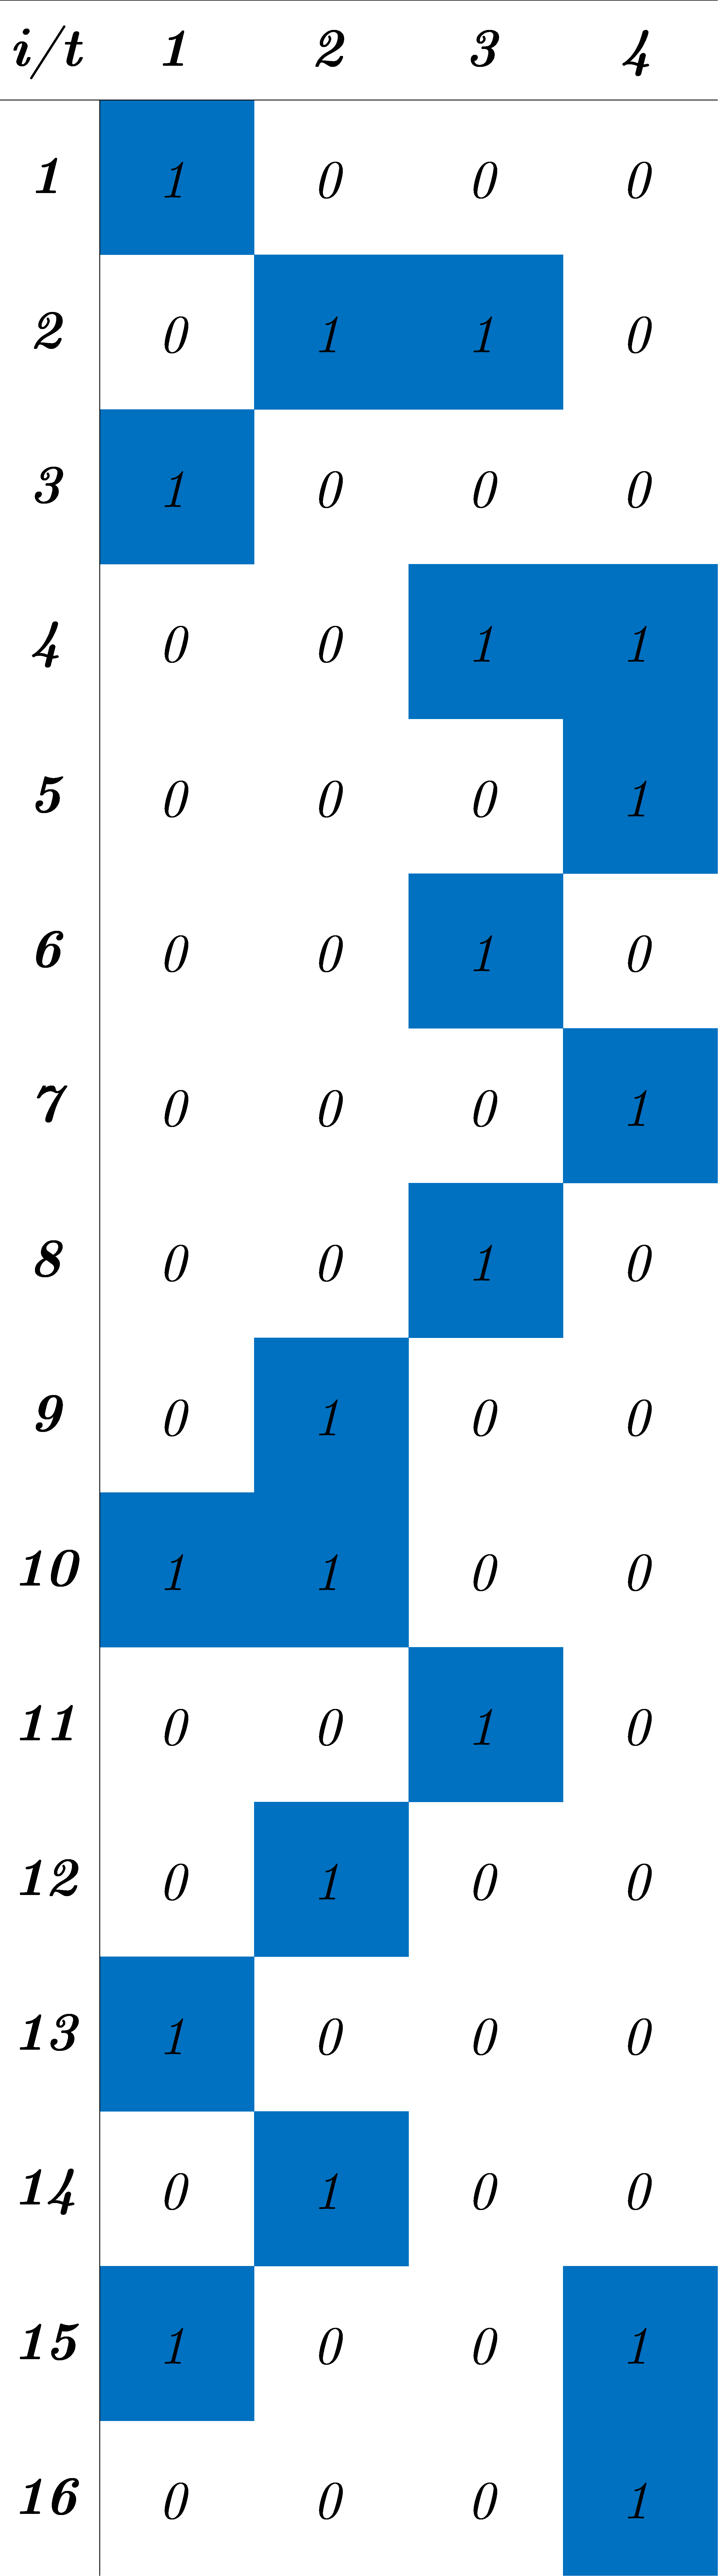
\includegraphics[width=5cm]{Figures/itemsxtests.png}
	\caption{An example of unbalanced \emph{items $\times$ tests} design, for $T=4$ tests with lenght equal to 5 and 2 anchor items (overlap), and $I=16$ items from the pool.}
	\label{fig:itemsxtests}
\end{figure}
\begin{figure}[ht]
	\centering
	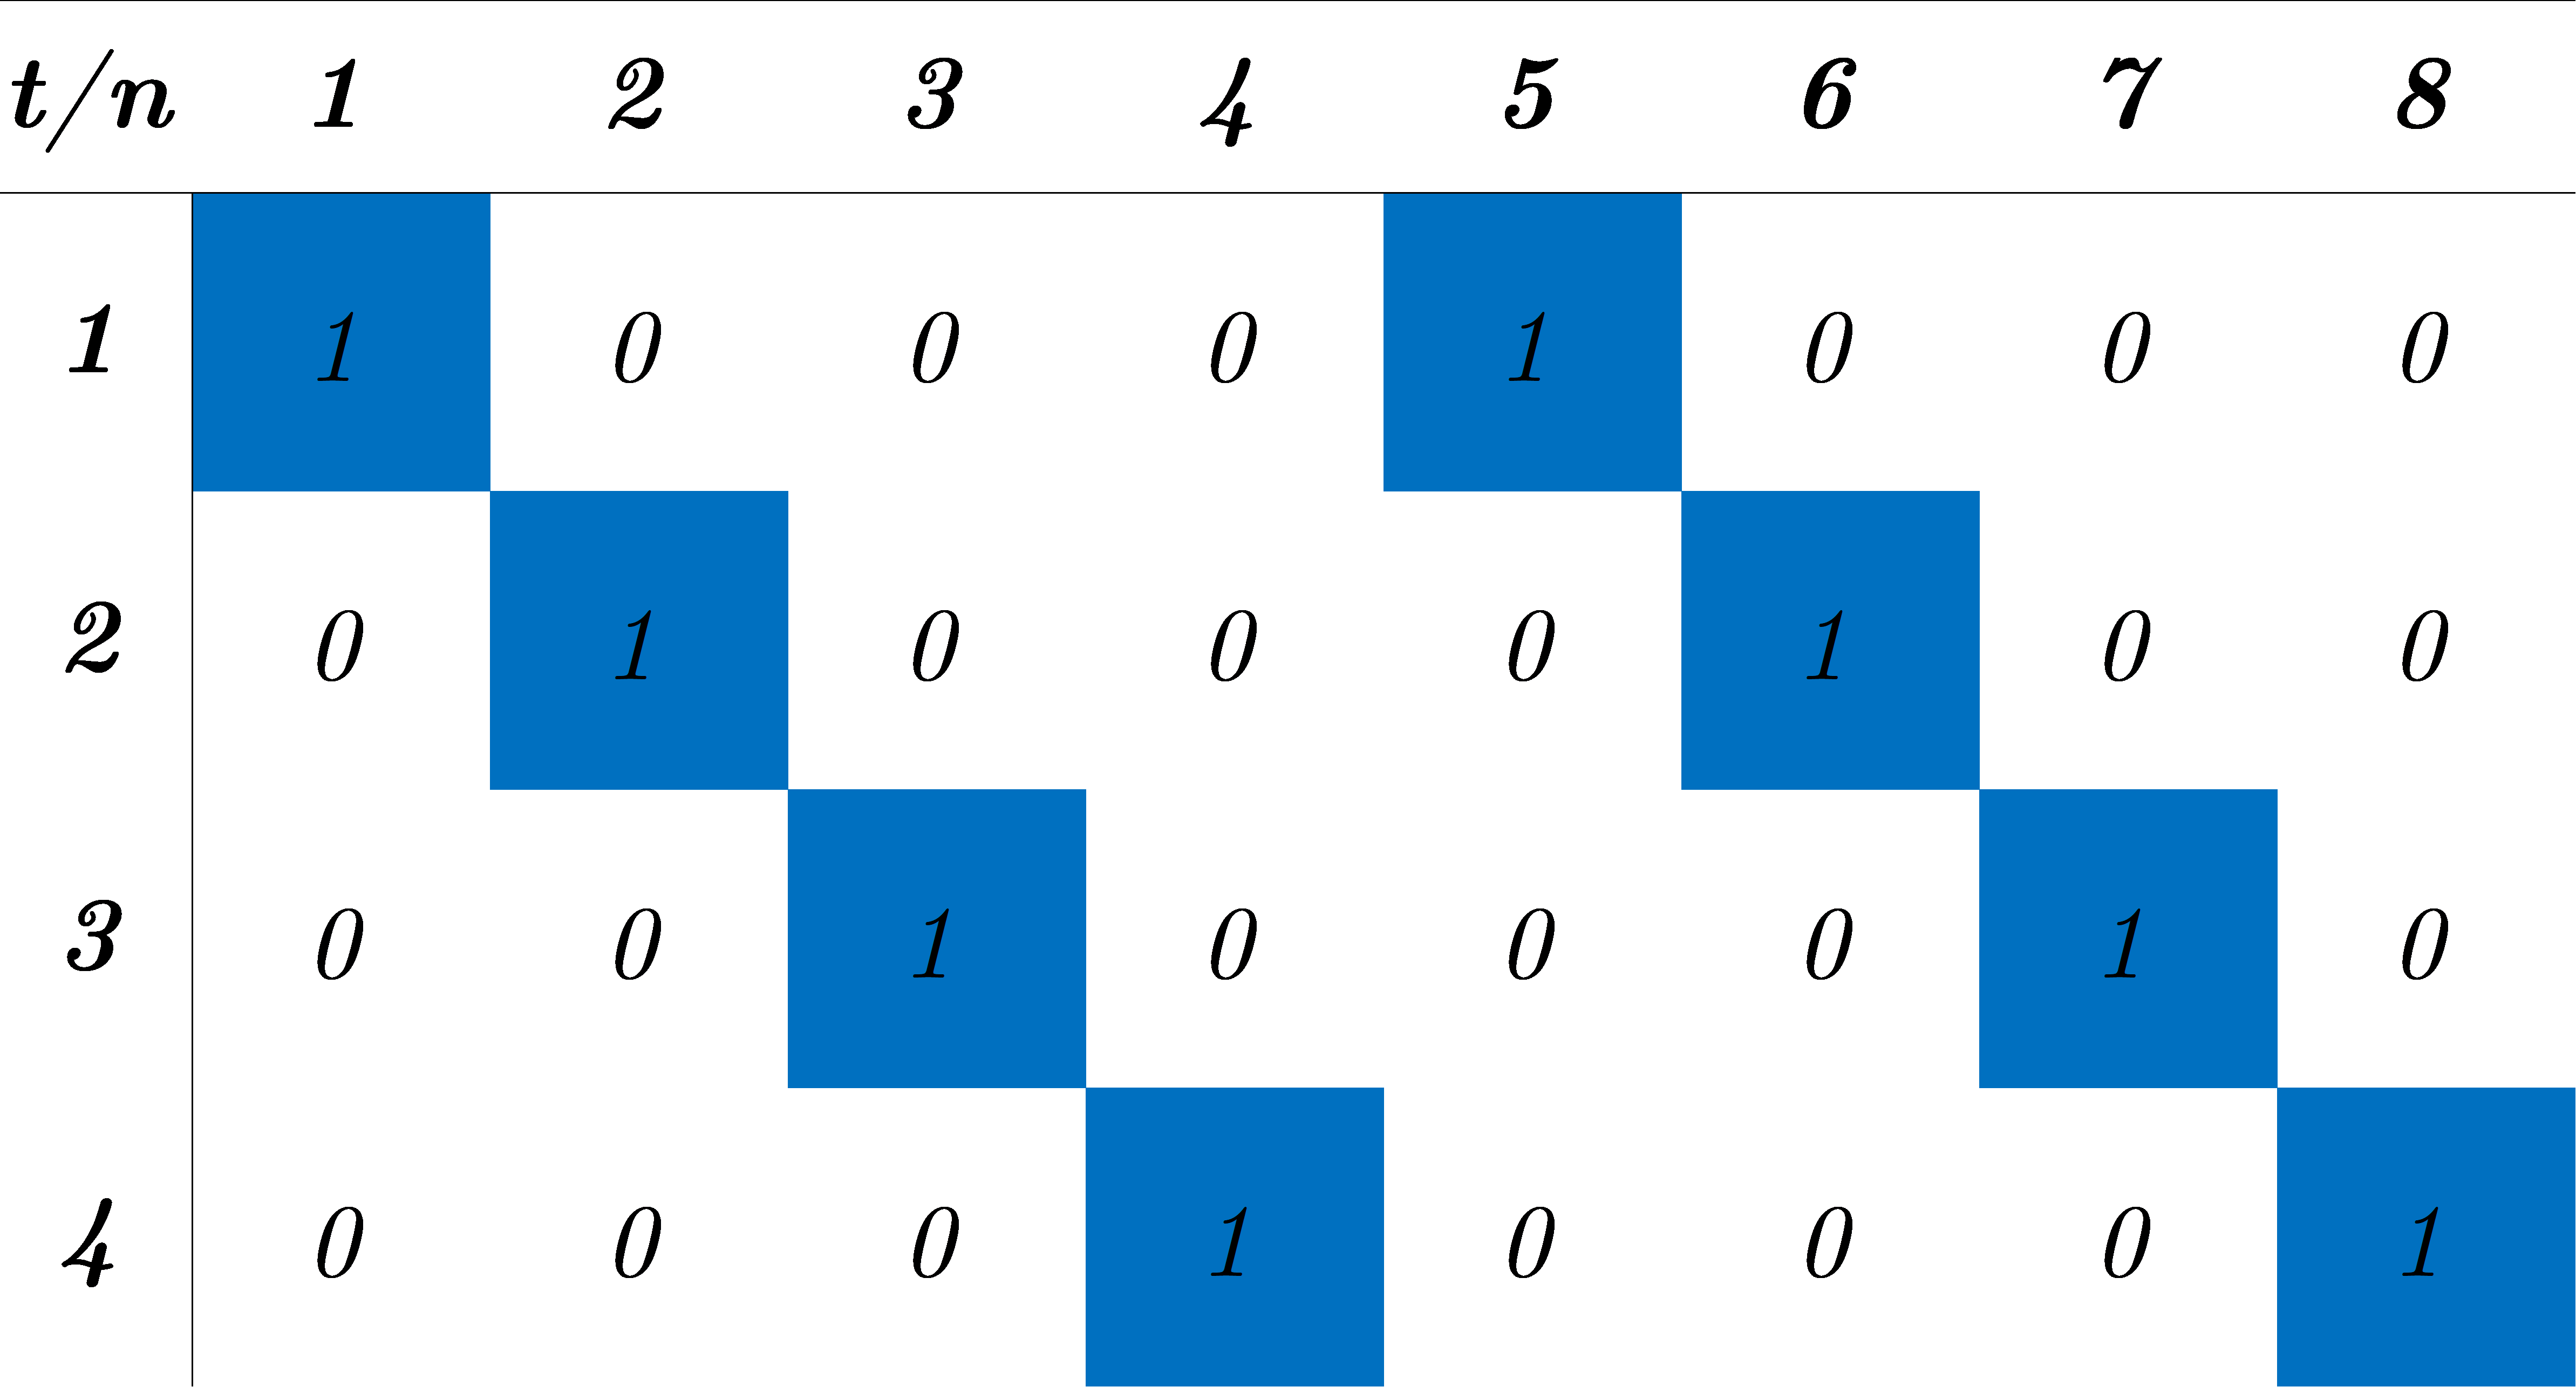
\includegraphics[width=10cm]{Figures/testsxexaminees.png}
	\caption{An example of \emph{tests $\times$ examinees} design, for $T=4$ tests, and $N=8$ test takers. To provide a random assignment we choose to distribute the tests in a sequential fashion.}
	\label{fig:testsxexaminees}
\end{figure}
\begin{figure}[ht]
	\centering
	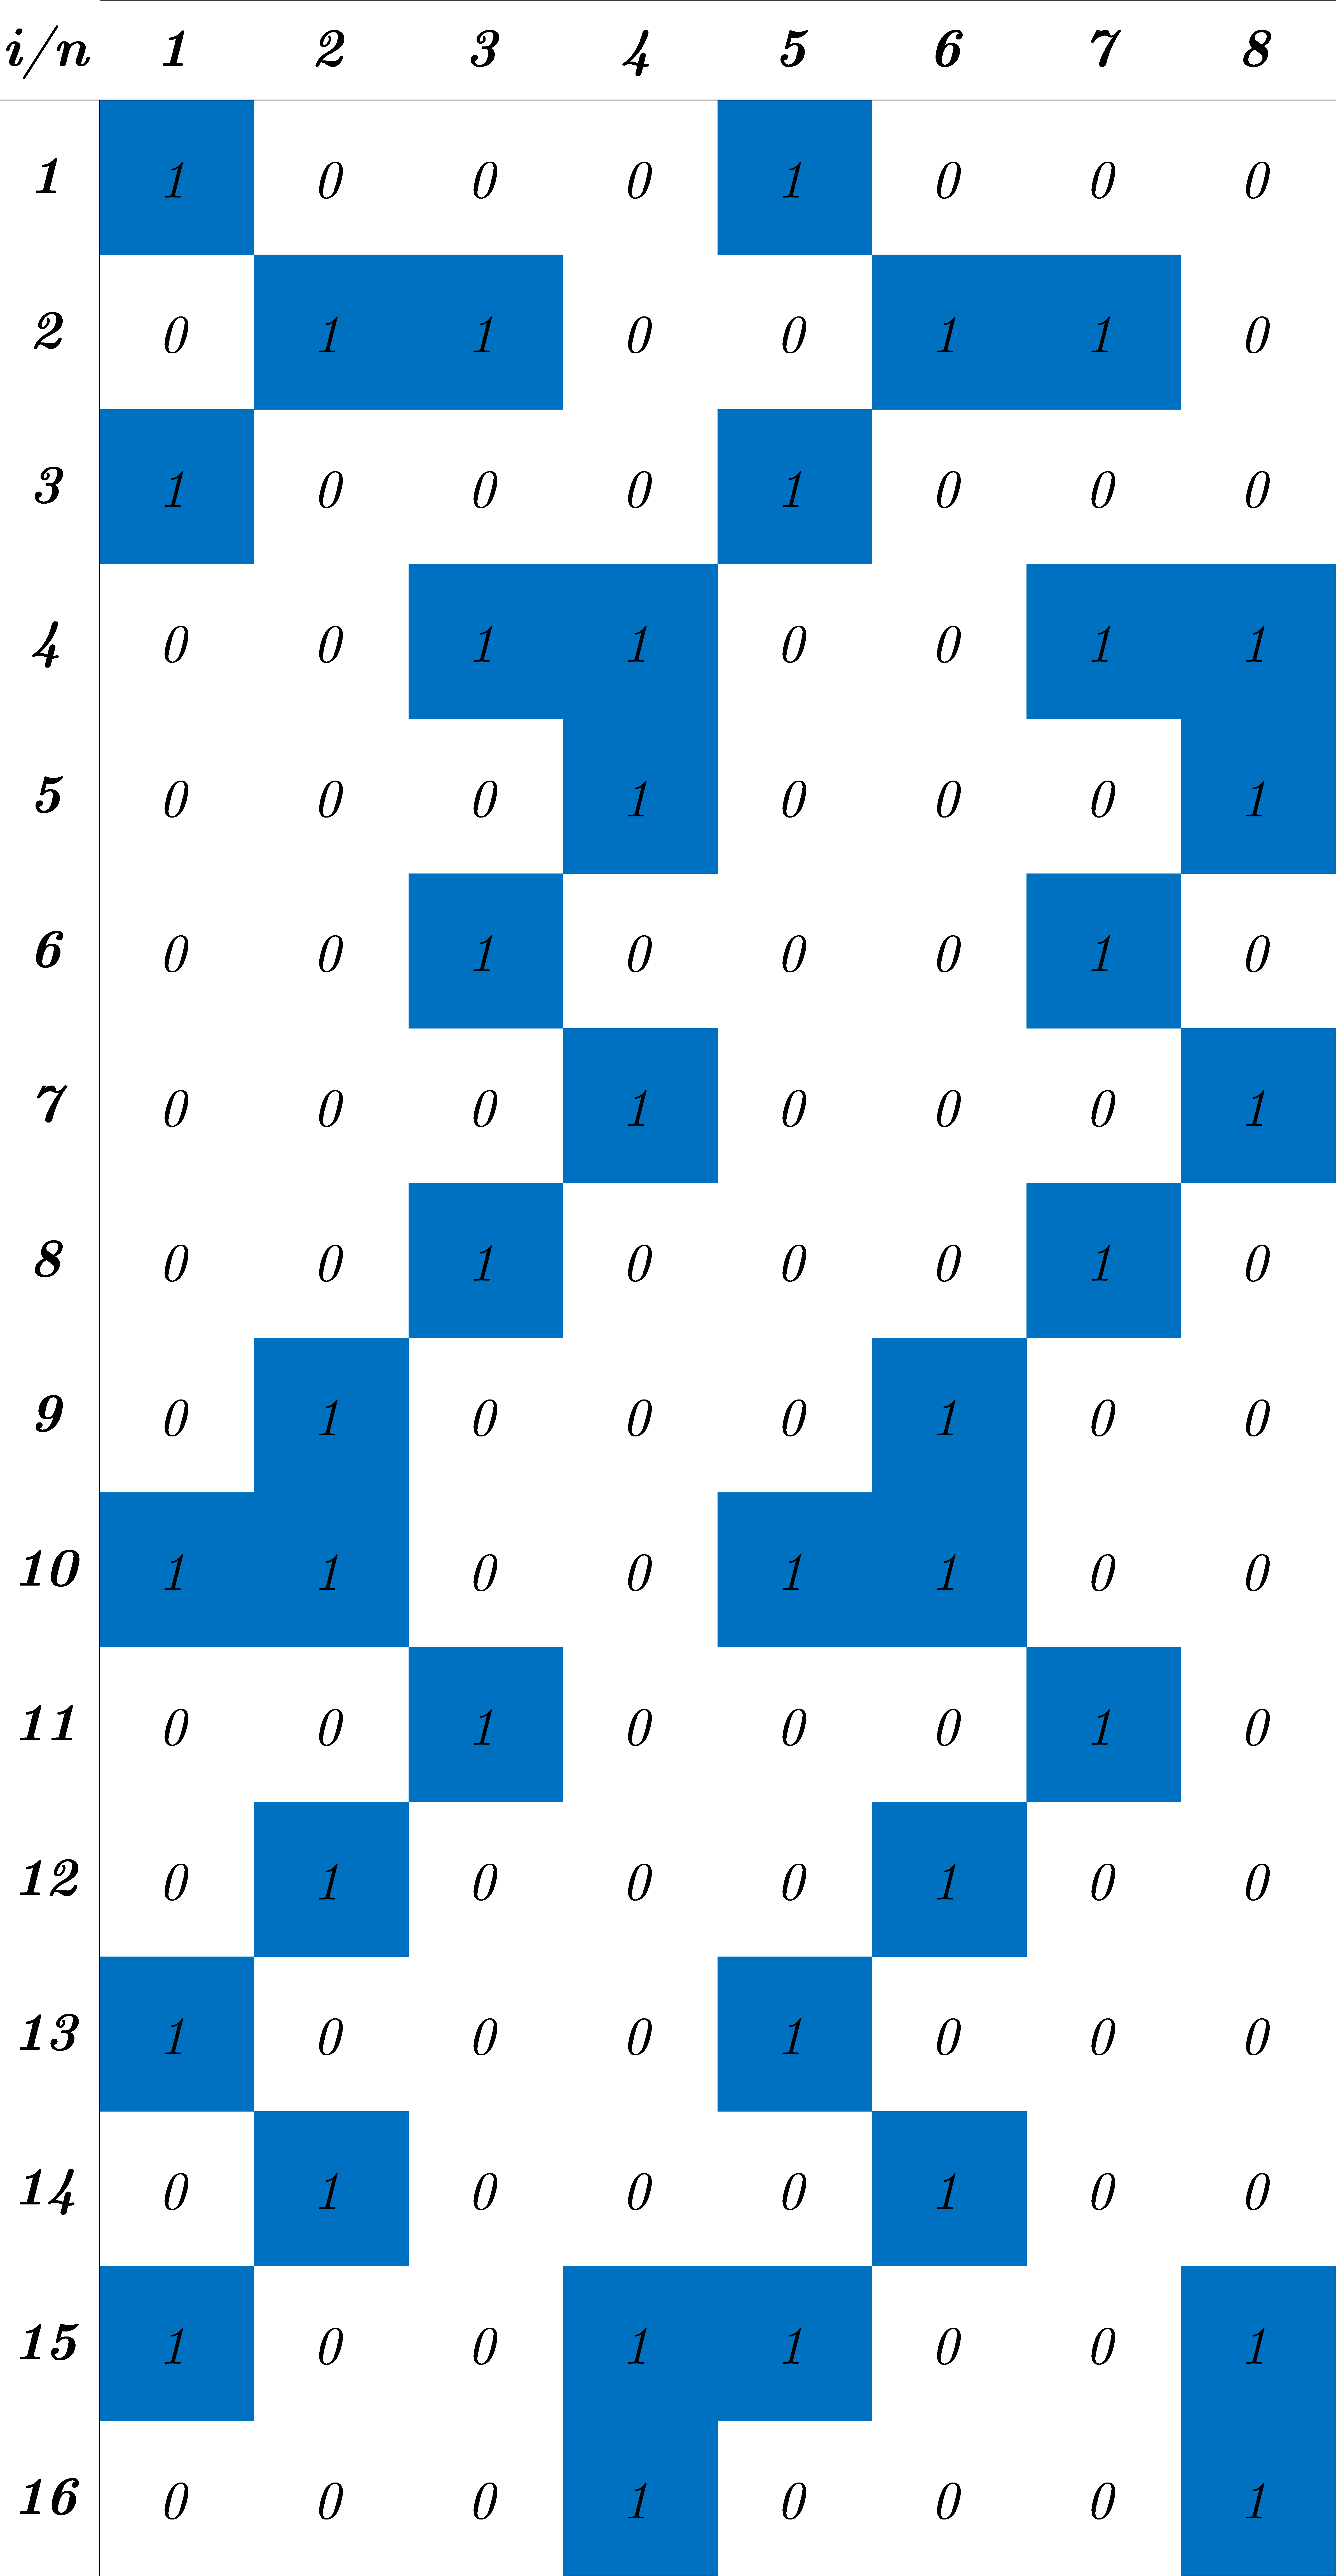
\includegraphics[width=10cm]{Figures/itemsxexaminees.png}
	\caption{An example of \emph{items $\times$ examinees} design, for $I=16$ items, and $N=8$ test takers.}
	\label{fig:itemsxexaminees}
\end{figure}


\section{Items calibration in Julia}
\subsection{Case 1a (Standard setup)}

\begin{sidewaystable}
	%\frac{p(X_k|\boldsymbol{u}_n,\boldsymbol{\tau},\hat{\boldsymbol{\xi}}^{(s)})W[k]}{\sum_{j=1}^K{p(X_j|\boldsymbol{u}_n,\boldsymbol{\tau},\hat{\boldsymbol{\xi}}^{(s)})W[j]}}
	\renewcommand{\arraystretch}{1}%
	\footnotesize
	\centering \begin{tabular}{|l|l|lll|lll|l|lll|lll}
		& &  \multicolumn{3}{c}{RMSE}& \multicolumn{3}{c}{BIAS}& & \multicolumn{3}{c}{RMSE}& \multicolumn{3}{c}{BIAS} \\
		i & $a_{true}$ & $a_{jl}$ & $a_{mirt}$ & $a_{mirt EHW}$ & $ a_{jl} $ & $ a_{mirt} $ & $ a_{mirt EHW} $ & $ b_{true} $ & $ b_{jl} $ & $ b_{mirt} $ & $ b_{mirt EHW} $ & $ b_{jl} $ & $b_{mirt}$ & $b_{mirt EHW}$\\
		\hline
		1 & 1.03 & 0.126 & 0.126 & 0.126 & 0.004 & -0.0 & -0.002 & -0.154 & 0.108 & 0.108 & 0.108 & -0.016 & -0.019 & -0.016 \\
		2 & 1.028 & 0.151 & 0.152 & 0.152 & 0.007 & 0.001 & -0.002 & 1.651 & 0.124 & 0.124 & 0.124 & 0.015 & 0.013 & 0.015 \\
		3 & 0.852 & 0.12 & 0.12 & 0.121 & -0.012 & -0.015 & -0.018 & -0.085 & 0.104 & 0.104 & 0.104 & -0.004 & -0.006 & -0.004 \\
		4 & 1.313 & 0.154 & 0.156 & 0.159 & -0.05 & -0.055 & -0.06 & .393 & 0.118 & 0.118 & 0.118 & 0.002 & -0.001 & 0.002 \\
		5 & 1.552 & 0.165 & 0.164 & 0.166 & 0.011 & 0.006 & 0.001 & -0.025 & 0.125 & 0.125 & 0.125 & -0.005 & -0.011 & -0.006 \\
		6 & 0.782 & 0.115 & 0.114 & 0.115 & 0.003 & -0.0 & -0.001 & -0.828 & 0.104 & 0.104 & 0.104 & -0.003 & -0.006 & -0.003 \\
		7 & 1.037 & 0.152 & 0.152 & 0.155 & -0.029 & -0.034 & -0.037 & 0.539 & 0.101 & 0.101 & 0.101 & -0.008 & -0.01 & -0.008 \\
		8 & 0.896 & 0.108 & 0.107 & 0.107 & 0.029 & 0.025 & 0.022 & 0.163 & 0.087 & 0.088 & 0.088 & -0.004 & -0.004 & -0.003 \\
		9 & 1.207 & 0.153 & 0.153 & 0.155 & -0.013 & -0.019 & -0.021 & 0.872 & 0.109 & 0.109 & 0.109 & -0.001 & -0.004 & -0.001 \\
		10 & 0.912 & 0.135 & 0.135 & 0.136 & 0.014 & 0.01 & 0.007 & -0.835 & 0.107 & 0.106 & 0.107 & 0.015 & 0.013 & 0.015 \\
		11 & 1.185 & 0.089 & 0.091 & 0.091 & -0.011 & -0.019 & -0.019 & 1.261 & 0.084 & 0.085 & 0.084 & -0.0 & -0.005 & -0.001 \\
		12 & 0.672 & 0.129 & 0.129 & 0.129 & 0.013 & 0.009 & 0.008 & 0.955 & 0.105 & 0.106 & 0.105 & -0.035 & -0.036 & -0.035 \\
		13 & 1.172 & 0.139 & 0.141 & 0.142 & -0.019 & -0.026 & -0.027 & 0.71 & 0.124 & 0.126 & 0.125 & -0.061 & -0.065 & -0.063 \\
		14 & 1.542 & 0.178 & 0.178 & 0.18 & -0.014 & -0.019 & -0.024 & -2.022 & 0.166 & 0.165 & 0.167 & 0.009 & 0.006 & 0.008 \\
		15 & 0.828 & 0.135 & 0.135 & 0.136 & -0.002 & -0.006 & -0.009 & -0.636 & 0.106 & 0.106 & 0.106 & 0.018 & 0.016 & 0.018 \\
		16 & 0.869 & 0.126 & 0.127 & 0.127 & -0.02 & -0.024 & -0.025 & 1.011 & 0.112 & 0.112 & 0.112 & -0.004 & -0.006 & -0.004 \\
		17 & 0.823 & 0.08 & 0.081 & 0.081 & -0.01 & -0.014 & -0.015 & -0.64 & 0.071 & 0.071 & 0.071 & 0.006 & 0.003 & 0.005 \\
		18 & 0.932 & 0.116 & 0.116 & 0.116 & 0.012 & 0.007 & 0.006 & 0.122 & 0.105 & 0.104 & 0.105 & 0.004 & 0.003 & 0.004 \\
		19 & 1.163 & 0.097 & 0.098 & 0.098 & -0.008 & -0.013 & -0.016 & 0.761 & 0.078 & 0.079 & 0.078 & -0.012 & -0.014 & -0.012 \\
		20 & 0.936 & 0.139 & 0.138 & 0.14 & 0.013 & 0.009 & 0.006 & -0.827 & 0.11 & 0.11 & 0.111 & 0.015 & 0.014 & 0.015 \\
		21 & 1.789 & 0.13 & 0.131 & 0.131 & -0.001 & -0.007 & -0.013 & 0.653 & 0.089 & 0.091 & 0.089 & -0.03 & -0.036 & -0.031 \\
		22 & 1.58 & 0.137 & 0.137 & 0.142 & -0.047 & -0.051 & -0.057 & -.364 & 0.082 & 0.081 & 0.082 & 0.021 & 0.017 & 0.02 \\
		23 & 1.248 & 0.146 & 0.146 & 0.146 & 0.021 & 0.016 & 0.013 & 0.424 & 0.122 & 0.123 & 0.122 & -0.015 & -0.019 & -0.015 \\
		24 & 0.618 & 0.124 & 0.125 & 0.125 & -0.006 & -0.01 & -0.01 & 0.441 & 0.103 & 0.103 & 0.103 & 0.004 & 0.003 & 0.004 \\
		25 & 0.757 & 0.115 & 0.115 & 0.115 & 0.011 & 0.007 & 0.006 & 0.082 & 0.1 & 0.099 & 0.1 & -0.002 & -0.002 & -0.002 \\
		26 & 0.916 & 0.143 & 0.144 & 0.144 & 0.011 & 0.006 & 0.004 & 2.277 & 0.132 & 0.134 & 0.133 & -0.01 & -0.013 & -0.011 \\
		27 & 1.36 & 0.14 & 0.141 & 0.142 & -0.014 & -0.019 & -0.023 & -0.087 & 0.114 & 0.114 & 0.113 & -0.013 & -0.017 & -0.015 \\
		28 & 0.769 & 0.133 & 0.133 & 0.134 & -0.001 & -0.006 & -0.006 & -1.576 & 0.126 & 0.126 & 0.126 & 0.003 & 0.001 & 0.003 \\
		29 & 0.909 & 0.1 & 0.101 & 0.103 & -0.032 & -0.036 & -0.038 & -0.013 & 0.071 & 0.071 & 0.071 & 0.015 & 0.013 & 0.015 \\
		30 & 1.082 & 0.146 & 0.146 & 0.147 & -0.018 & -0.022 & -0.024 & -0.595 & 0.118 & 0.117 & 0.118 & 0.009 & 0.005 & 0.008 \\
		31 & 0.925 & 0.136 & 0.139 & 0.138 & -0.014 & -0.019 & -0.02 & 0.807 & 0.111 & 0.111 & 0.111 & 0.013 & 0.01 & 0.012 \\
		32 & 0.748 & 0.109 & 0.11 & 0.11 & 0.003 & -0.0 & -0.001 & -.328 & 0.092 & 0.092 & 0.092 & 0.006 & 0.003 & 0.005 \\
		33 & 0.764 & 0.119 & 0.12 & 0.12 & -0.002 & -0.006 & -0.008 & 0.88 & 0.095 & 0.095 & 0.095 & 0.008 & 0.006 & 0.008 \\
		34 & 1.167 & 0.141 & 0.141 & 0.142 & -0.01 & -0.014 & -0.017 & -0.181 & 0.115 & 0.116 & 0.115 & -0.035 & -0.039 & -0.037 \\
		35 & 1.272 & .313 & .313 & .316 & -0.051 & -0.059 & -0.058 & -2.73 & .343 & .343 & .341 & 0.042 & 0.039 & 0.038 \\
		36 & 1.211 & 0.14 & 0.14 & 0.141 & -0.004 & -0.008 & -0.013 & -0.031 & 0.102 & 0.102 & 0.102 & 0.017 & 0.015 & 0.017 \\
		37 & 1.748 & 0.197 & 0.197 & .302 & -0.065 & -0.069 & -0.078 & -0.419 & 0.118 & 0.118 & 0.118 & 0.004 & -0.0 & 0.003 
	\end{tabular}

\end{sidewaystable}
\begin{sidewaystable}
	%\frac{p(X_k|\boldsymbol{u}_n,\boldsymbol{\tau},\hat{\boldsymbol{\xi}}^{(s)})W[k]}{\sum_{j=1}^K{p(X_j|\boldsymbol{u}_n,\boldsymbol{\tau},\hat{\boldsymbol{\xi}}^{(s)})W[j]}}
	\renewcommand{\arraystretch}{1}%
	\footnotesize
	\centering \begin{tabular}{|l|l|lll|lll|l|lll|lll}
		& &  \multicolumn{3}{c}{RMSE}& \multicolumn{3}{c}{BIAS}& & \multicolumn{3}{c}{RMSE}& \multicolumn{3}{c}{BIAS} \\
		i & $a_{true}$ & $a_{jl}$ & $a_{mirt}$ & $a_{mirt EHW}$ & $ a_{jl} $ & $ a_{mirt} $ & $ a_{mirt EHW} $ & $ b_{true} $ & $ b_{jl} $ & $ b_{mirt} $ & $ b_{mirt EHW} $ & $ b_{jl} $ & $b_{mirt}$ & $b_{mirt EHW}$\\
		\hline
		38 & 0.598 & 0.175 & 0.176 & 0.176 & 0.0 & -0.005 & -0.003 & -2.013 & 0.158 & 0.158 & 0.158 & 0.022 & 0.021 & 0.022 \\
		39 & 1.045 & 0.125 & 0.124 & 0.126 & 0.001 & -0.004 & -0.006 & -1.122 & 0.113 & 0.114 & 0.114 & -0.026 & -0.029 & -0.027 \\
		40 & 0.637 & 0.132 & 0.132 & 0.133 & -0.002 & -0.006 & -0.006 & -1.46 & 0.117 & 0.117 & 0.117 & 0.01 & 0.007 & 0.009 	\\
		
		41 & 1.628 & .301 & .302 & .304 & -0.021 & -0.031 & -0.032 & 1.35 & 0.14 & 0.14 & 0.141 & 0.027 & 0.02 & 0.026 \\
		42 & 0.877 & 0.121 & 0.12 & 0.12 & 0.027 & 0.022 & 0.02 & 0.509 & 0.115 & 0.116 & 0.115 & -0.01 & -0.011 & -0.01 \\
		43 & 0.734 & 0.126 & 0.128 & 0.128 & -0.022 & -0.026 & -0.026 & -0.001 & 0.095 & 0.095 & 0.095 & 0.007 & 0.005 & 0.007 \\
		44 & 0.636 & 0.076 & 0.076 & 0.076 & 0.011 & 0.008 & 0.007 & .303 & 0.065 & 0.065 & 0.065 & 0.0 & -0.001 & 0.0 \\
		45 & 1.072 & 0.094 & 0.095 & 0.097 & -0.022 & -0.026 & -0.03 & -0.981 & 0.087 & 0.087 & 0.087 & 0.011 & 0.01 & 0.011 \\
		46 & 0.923 & 0.133 & 0.133 & 0.134 & -0.002 & -0.005 & -0.009 & -0.31 & 0.111 & 0.11 & 0.111 & 0.016 & 0.014 & 0.016 \\
		47 & 1.547 & 0.166 & 0.169 & 0.17 & -0.022 & -0.03 & -0.033 & 0.901 & 0.12 & 0.12 & 0.121 & 0.004 & 0.001 & 0.005 \\
		48 & 1.479 & 0.182 & 0.183 & 0.183 & 0.009 & 0.005 & -0.001 & -0.584 & 0.12 & 0.119 & 0.119 & 0.02 & 0.018 & 0.02 \\
		49 & 1.108 & 0.137 & 0.137 & 0.136 & 0.023 & 0.019 & 0.016 & -0.768 & 0.109 & 0.111 & 0.109 & -0.043 & -0.047 & -0.045 \\
		50 & 0.701 & 0.126 & 0.127 & 0.126 & -0.003 & -0.007 & -0.007 & 0.857 & 0.112 & 0.113 & 0.112 & -0.026 & -0.028 & -0.027 \\
		51 & 0.745 & 0.108 & 0.108 & 0.108 & 0.012 & 0.008 & 0.007 & .308 & 0.087 & 0.087 & 0.087 & -0.001 & -0.004 & -0.001 \\
		52 & 1.041 & 0.102 & 0.102 & 0.103 & -0.001 & -0.004 & -0.008 & -0.568 & 0.074 & 0.074 & 0.074 & 0.005 & 0.003 & 0.005 \\
		53 & 1.337 & 0.138 & 0.139 & 0.141 & -0.034 & -0.038 & -0.043 & -0.059 & 0.104 & 0.105 & 0.104 & -0.007 & -0.01 & -0.007 \\
		54 & 0.556 & 0.133 & 0.134 & 0.134 & -0.011 & -0.014 & -0.014 & -1.985 & 0.136 & 0.136 & 0.136 & 0.006 & 0.005 & 0.006 \\
		55 & 0.986 & 0.132 & 0.132 & 0.132 & 0.014 & 0.009 & 0.008 & -1.001 & 0.112 & 0.112 & 0.112 & 0.013 & 0.01 & 0.012 \\
		56 & 0.758 & 0.108 & 0.107 & 0.108 & 0.025 & 0.021 & 0.02 & .342 & 0.098 & 0.098 & 0.098 & 0.005 & 0.005 & 0.005 \\
		57 & 0.609 & 0.107 & 0.108 & 0.108 & 0.001 & -0.002 & -0.003 & 0.975 & 0.117 & 0.117 & 0.117 & 0.017 & 0.016 & 0.017 \\
		58 & 1.427 & .306 & .306 & .308 & -0.004 & -0.009 & -0.013 & -2.69 & .325 & .323 & .325 & 0.017 & 0.014 & 0.016 \\
		59 & 0.855 & 0.11 & 0.109 & 0.111 & 0.003 & -0.001 & -0.002 & -.349 & 0.112 & 0.113 & 0.113 & -0.039 & -0.041 & -0.04 \\
		60 & 1.494 & 0.197 & 0.197 & 0.197 & 0.021 & 0.013 & 0.012 & 1.068 & 0.115 & 0.118 & 0.116 & -0.013 & -0.019 & -0.014 \\
		61 & 1.839 & .305 & .303 & .303 & 0.048 & 0.044 & 0.036 & -0.076 & 0.119 & 0.119 & 0.119 & -0.002 & -0.004 & -0.001 \\
		62 & 1.229 & 0.118 & 0.118 & 0.117 & 0.038 & 0.034 & 0.03 & -0.685 & 0.08 & 0.08 & 0.08 & 0.005 & 0.004 & 0.005 \\
		63 & 0.865 & 0.135 & 0.137 & 0.136 & -0.011 & -0.016 & -0.017 & -.364 & 0.099 & 0.099 & 0.099 & 0.01 & 0.007 & 0.009 \\
		64 & 0.747 & 0.114 & 0.116 & 0.116 & -0.03 & -0.034 & -0.035 & 0.652 & 0.112 & 0.112 & 0.112 & -0.029 & -0.032 & -0.03 \\
		65 & 1.201 & 0.138 & 0.136 & 0.139 & 0.009 & 0.006 & 0.0 & -.314 & 0.102 & 0.102 & 0.103 & 0.022 & 0.019 & 0.022 \\
		66 & 1.151 & 0.138 & 0.138 & 0.137 & 0.027 & 0.022 & 0.02 & -0.055 & 0.103 & 0.104 & 0.103 & 0.002 & -0.002 & 0.001 \\
		67 & 0.982 & 0.099 & 0.099 & 0.099 & 0.014 & 0.01 & 0.008 & -0.63 & 0.068 & 0.069 & 0.068 & -0.022 & -0.025 & -0.023 \\
		68 & 0.866 & 0.13 & 0.131 & 0.131 & -0.018 & -0.023 & -0.024 & -0.775 & 0.104 & 0.104 & 0.104 & 0.008 & 0.006 & 0.008 \\
		69 & 0.738 & 0.117 & 0.117 & 0.119 & -0.004 & -0.008 & -0.01 & 1.163 & 0.108 & 0.108 & 0.108 & 0.003 & 0.001 & 0.003 \\
		70 & 1.19 & 0.152 & 0.152 & 0.154 & -0.003 & -0.01 & -0.011 & 0.966 & 0.12 & 0.121 & 0.12 & -0.043 & -0.048 & -0.045 \\
		71 & 1.236 & 0.139 & 0.139 & 0.141 & -0.008 & -0.012 & -0.016 & -0.646 & 0.112 & 0.113 & 0.112 & -0.007 & -0.009 & -0.007 \\
		72 & 1.52 & 0.163 & 0.162 & 0.163 & 0.032 & 0.027 & 0.021 & 0.156 & 0.113 & 0.113 & 0.113 & 0.029 & 0.027 & 0.029 \\
		73 & 1.021 & 0.102 & 0.101 & 0.102 & 0.017 & 0.01 & 0.011 & 1.658 & 0.099 & 0.099 & 0.099 & 0.011 & 0.008 & 0.011 \\
		74 & 1.037 & 0.15 & 0.151 & 0.152 & -0.026 & -0.032 & -0.033 & .333 & 0.1 & 0.1 & 0.1 & 0.007 & 0.004 & 0.007 
	\end{tabular}
	
\end{sidewaystable}
\begin{sidewaystable}
	%\frac{p(X_k|\boldsymbol{u}_n,\boldsymbol{\tau},\hat{\boldsymbol{\xi}}^{(s)})W[k]}{\sum_{j=1}^K{p(X_j|\boldsymbol{u}_n,\boldsymbol{\tau},\hat{\boldsymbol{\xi}}^{(s)})W[j]}}
	\renewcommand{\arraystretch}{1}%
	\footnotesize
	\centering \begin{tabular}{|l|l|lll|lll|l|lll|lll}
		& &  \multicolumn{3}{c}{RMSE}& \multicolumn{3}{c}{BIAS}& & \multicolumn{3}{c}{RMSE}& \multicolumn{3}{c}{BIAS} \\
		i & $a_{true}$ & $a_{jl}$ & $a_{mirt}$ & $a_{mirt EHW}$ & $ a_{jl} $ & $ a_{mirt} $ & $ a_{mirt EHW} $ & $ b_{true} $ & $ b_{jl} $ & $ b_{mirt} $ & $ b_{mirt EHW} $ & $ b_{jl} $ & $b_{mirt}$ & $b_{mirt EHW}$\\
		\hline
		75 & 1.547 & .308 & .307 & .309 & 0.003 & -0.005 & -0.006 & -2.704 & .314 & .314 & .315 & -0.039 & -0.043 & -0.042 \\
		76 & 1.021 & 0.149 & 0.149 & 0.15 & 0.019 & 0.014 & 0.013 & 0.996 & 0.124 & 0.125 & 0.124 & -0.004 & -0.008 & -0.005 \\
		77 & 1.814 & 0.133 & 0.133 & 0.134 & 0.002 & -0.006 & -0.01 & 1.055 & 0.108 & 0.106 & 0.107 & 0.022 & 0.015 & 0.021 \\
		78 & 0.996 & 0.137 & 0.141 & 0.139 & -0.016 & -0.023 & -0.023 & 1.774 & 0.175 & 0.176 & 0.175 & -0.059 & -0.062 & -0.06 \\
		79 & 0.841 & 0.128 & 0.129 & 0.13 & -0.03 & -0.035 & -0.037 & 0.82 & 0.106 & 0.106 & 0.106 & -0.002 & -0.003 & -0.002 \\
		80 & 0.946 & 0.13 & 0.129 & 0.131 & 0.012 & 0.008 & 0.005 & -1.351 & 0.128 & 0.128 & 0.129 & 0.017 & 0.016 & 0.017 \\
		81 & 1.317 & 0.158 & 0.158 & 0.16 & -0.006 & -0.011 & -0.015 & -0.652 & 0.114 & 0.113 & 0.114 & 0.025 & 0.022 & 0.025 \\
		82 & 1.117 & 0.144 & 0.144 & 0.145 & 0.001 & -0.004 & -0.006 & -1.044 & 0.112 & 0.114 & 0.113 & -0.027 & -0.031 & -0.029 \\
		83 & 0.779 & 0.137 & 0.137 & 0.138 & -0.005 & -0.009 & -0.012 & 0.697 & 0.105 & 0.105 & 0.106 & 0.027 & 0.025 & 0.027 \\
		84 & 0.768 & 0.126 & 0.127 & 0.128 & -0.015 & -0.019 & -0.02 & -0.363 & 0.091 & 0.09 & 0.091 & 0.004 & 0.003 & 0.004 \\
		85 & 1.522 & 0.1 & 0.102 & 0.102 & -0.007 & -0.013 & -0.017 & 0.414 & 0.072 & 0.071 & 0.072 & 0.011 & 0.007 & 0.01 \\
		86 & 0.819 & 0.069 & 0.07 & 0.07 & -0.006 & -0.01 & -0.012 & 0.348 & 0.064 & 0.063 & 0.064 & 0.007 & 0.006 & 0.007 \\
		87 & 1.714 & 0.179 & 0.177 & 0.179 & 0.028 & 0.022 & 0.016 & 0.515 & 0.114 & 0.114 & 0.114 & -0.006 & -0.009 & -0.006 \\
		88 & 0.928 & 0.126 & 0.126 & 0.127 & 0.003 & -0.002 & -0.003 & 0.374 & 0.118 & 0.118 & 0.118 & -0.011 & -0.014 & -0.011 \\
		89 & 0.591 & 0.091 & 0.092 & 0.092 & -0.012 & -0.015 & -0.016 & 0.077 & 0.092 & 0.093 & 0.093 & -0.006 & -0.007 & -0.006 \\
		90 & 0.803 & 0.132 & 0.131 & 0.132 & 0.022 & 0.016 & 0.016 & 1.614 & 0.138 & 0.138 & 0.138 & 0.012 & 0.011 & 0.012 \\
		91 & 0.977 & 0.134 & 0.133 & 0.133 & 0.049 & 0.045 & 0.042 & -1.44 & 0.124 & 0.124 & 0.124 & 0.018 & 0.017 & 0.019 \\
		92 & 1.435 & 0.117 & 0.116 & 0.117 & 0.021 & 0.015 & 0.012 & 0.586 & 0.086 & 0.088 & 0.086 & -0.028 & -0.033 & -0.029 \\
		93 & 0.776 & 0.148 & 0.15 & 0.15 & -0.013 & -0.018 & -0.019 & 2.543 & 0.156 & 0.157 & 0.156 & -0.026 & -0.028 & -0.027 \\
		94 & 1.413 & 0.164 & 0.166 & 0.167 & -0.016 & -0.024 & -0.026 & 0.744 & 0.115 & 0.115 & 0.115 & 0.015 & 0.01 & 0.014 \\
		95 & 1.039 & 0.131 & 0.131 & 0.131 & 0.013 & 0.009 & 0.007 & -0.326 & 0.1 & 0.101 & 0.1 & -0.013 & -0.016 & -0.014 \\
		96 & 0.769 & 0.11 & 0.11 & 0.111 & 0.008 & 0.005 & 0.004 & -0.48 & 0.091 & 0.091 & 0.091 & -0.007 & -0.009 & -0.008 \\
		97 & 0.957 & 0.132 & 0.131 & 0.132 & 0.015 & 0.01 & 0.01 & 0.871 & 0.098 & 0.099 & 0.098 & -0.007 & -0.01 & -0.007 \\
		98 & 1.31 & 0.148 & 0.149 & 0.149 & -0.003 & -0.007 & -0.011 & -1.123 & 0.126 & 0.126 & 0.126 & -0.021 & -0.023 & -0.021 \\
		99 & 1.702 & 0.122 & 0.121 & 0.123 & 0.012 & 0.007 & 0.001 & 0.115 & 0.088 & 0.09 & 0.089 & -0.013 & -0.018 & -0.014 \\
		100 & 1.052 & 0.142 & 0.142 & 0.143 & -0.002 & -0.006 & -0.01 & -.357 & 0.111 & 0.111 & 0.112 & 0.003 & 0.001 & 0.003 \\
		101 & 1.033 & 0.097 & 0.097 & 0.097 & 0.013 & 0.009 & 0.007 & 0.005 & 0.069 & 0.068 & 0.068 & 0.012 & 0.009 & 0.012 \\
		102 & 1.131 & 0.14 & 0.14 & 0.143 & -0.031 & -0.035 & -0.038 & -0.753 & 0.116 & 0.115 & 0.116 & 0.013 & 0.01 & 0.012 \\
		103 & 0.941 & 0.096 & 0.096 & 0.096 & 0.004 & 0.0 & -0.003 & .312 & 0.072 & 0.073 & 0.072 & -0.003 & -0.005 & -0.003 \\
		104 & 1.344 & 0.141 & 0.142 & 0.143 & -0.009 & -0.012 & -0.019 & -0.523 & 0.119 & 0.118 & 0.119 & 0.039 & 0.036 & 0.039 \\
		105 & 0.929 & 0.124 & 0.126 & 0.126 & -0.015 & -0.02 & -0.021 & .337 & 0.106 & 0.105 & 0.106 & 0.036 & 0.033 & 0.036 \\
		106 & 1.271 & 0.168 & 0.168 & 0.168 & 0.038 & 0.033 & 0.029 & -1.183 & 0.144 & 0.143 & 0.144 & 0.003 & 0.001 & 0.003 \\
		107 & 1.275 & 0.16 & 0.16 & 0.161 & 0.012 & 0.006 & 0.003 & 0.59 & 0.109 & 0.109 & 0.109 & -0.022 & -0.024 & -0.022 \\
		108 & 1.215 & 0.14 & 0.14 & 0.142 & -0.011 & -0.016 & -0.019 & -0.616 & 0.139 & 0.14 & 0.139 & -0.041 & -0.045 & -0.043 \\
		109 & 1.113 & 0.153 & 0.153 & 0.154 & 0.0 & -0.003 & -0.008 & -0.989 & 0.118 & 0.118 & 0.118 & 0.01 & 0.008 & 0.011 \\
		110 & 1.793 & 0.124 & 0.124 & 0.124 & 0.005 & 0.001 & -0.008 & -.373 & 0.086 & 0.085 & 0.086 & 0.012 & 0.009 & 0.013 \\
		111 & 0.776 & 0.126 & 0.126 & 0.128 & -0.01 & -0.014 & -0.015 & -1.098 & 0.104 & 0.104 & 0.104 & -0.01 & -0.012 & -0.011 
	\end{tabular}
	
\end{sidewaystable}
\begin{sidewaystable}
	%\frac{p(X_k|\boldsymbol{u}_n,\boldsymbol{\tau},\hat{\boldsymbol{\xi}}^{(s)})W[k]}{\sum_{j=1}^K{p(X_j|\boldsymbol{u}_n,\boldsymbol{\tau},\hat{\boldsymbol{\xi}}^{(s)})W[j]}}
	\renewcommand{\arraystretch}{1}%
	\footnotesize
	\centering \begin{tabular}{|l|l|lll|lll|l|lll|lll}
		& &  \multicolumn{3}{c}{RMSE}& \multicolumn{3}{c}{BIAS}& & \multicolumn{3}{c}{RMSE}& \multicolumn{3}{c}{BIAS} \\
		i & $a_{true}$ & $a_{jl}$ & $a_{mirt}$ & $a_{mirt EHW}$ & $ a_{jl} $ & $ a_{mirt} $ & $ a_{mirt EHW} $ & $ b_{true} $ & $ b_{jl} $ & $ b_{mirt} $ & $ b_{mirt EHW} $ & $ b_{jl} $ & $b_{mirt}$ & $b_{mirt EHW}$\\
		\hline
		112 & 1.044 & 0.141 & 0.14 & 0.142 & -0.001 & -0.006 & -0.008 & 0.505 & 0.106 & 0.106 & 0.106 & 0.013 & 0.011 & 0.013 \\
		113 & 0.82 & 0.086 & 0.087 & 0.088 & -0.013 & -0.017 & -0.018 & -0.527 & 0.063 & 0.063 & 0.063 & 0.008 & 0.005 & 0.008 \\
		114 & 1.109 & 0.141 & 0.14 & 0.141 & 0.018 & 0.014 & 0.01 & 0.03 & 0.107 & 0.107 & 0.107 & -0.005 & -0.007 & -0.005 \\
		115 & 0.695 & 0.092 & 0.093 & 0.094 & -0.015 & -0.018 & -0.02 & 0.632 & 0.083 & 0.083 & 0.083 & 0.012 & 0.01 & 0.012 \\
		116 & 0.823 & 0.127 & 0.129 & 0.13 & -0.039 & -0.044 & -0.044 & 1.01 & 0.114 & 0.114 & 0.114 & 0.018 & 0.016 & 0.018 \\
		117 & 1.063 & 0.108 & 0.107 & 0.106 & 0.037 & 0.033 & 0.03 & -0.477 & 0.103 & 0.103 & 0.103 & -0.006 & -0.007 & -0.005 \\
		118 & 1.485 & 0.149 & 0.148 & 0.153 & -0.029 & -0.034 & -0.04 & -0.053 & 0.131 & 0.133 & 0.132 & -0.045 & -0.05 & -0.047 \\
		119 & 0.858 & 0.12 & 0.12 & 0.122 & -0.007 & -0.011 & -0.013 & -0.039 & 0.094 & 0.094 & 0.094 & -0.006 & -0.007 & -0.006 \\
		120 & 1.022 & 0.146 & 0.146 & 0.146 & 0.017 & 0.01 & 0.01 & 1.612 & 0.137 & 0.139 & 0.138 & -0.031 & -0.034 & -0.032 \\
		121 & 1.215 & 0.15 & 0.15 & 0.151 & 0.006 & 0.002 & -0.001 & -.317 & 0.118 & 0.119 & 0.119 & -0.036 & -0.039 & -0.037 \\
		122 & 0.798 & 0.127 & 0.126 & 0.127 & 0.004 & 0.0 & -0.001 & -1.203 & 0.112 & 0.111 & 0.112 & 0.009 & 0.008 & 0.009 \\
		123 & 0.934 & 0.108 & 0.108 & 0.109 & -0.007 & -0.012 & -0.015 & 1.059 & 0.084 & 0.085 & 0.084 & -0.012 & -0.014 & -0.012 \\
		124 & 1.574 & 0.156 & 0.156 & 0.157 & 0.002 & -0.004 & -0.009 & 0.377 & 0.107 & 0.107 & 0.107 & -0.008 & -0.01 & -0.007 \\
		125 & 0.855 & 0.109 & 0.109 & 0.111 & -0.008 & -0.012 & -0.013 & 0.142 & 0.096 & 0.097 & 0.096 & -0.019 & -0.021 & -0.02 \\
		126 & 0.843 & 0.12 & 0.121 & 0.121 & 0.006 & 0.002 & 0.001 & -0.966 & 0.106 & 0.106 & 0.106 & 0.026 & 0.025 & 0.026 \\
		127 & 1.047 & 0.102 & 0.101 & 0.102 & 0.016 & 0.011 & 0.009 & -0.379 & 0.086 & 0.087 & 0.087 & -0.015 & -0.018 & -0.015 \\
		128 & 0.905 & 0.144 & 0.144 & 0.146 & -0.007 & -0.01 & -0.013 & -1.35 & 0.128 & 0.128 & 0.127 & -0.003 & -0.005 & -0.003 \\
		129 & 1.149 & 0.1 & 0.1 & 0.102 & -0.006 & -0.013 & -0.014 & 0.931 & 0.089 & 0.089 & 0.089 & 0.019 & 0.016 & 0.019 \\
		130 & 1.453 & 0.113 & 0.113 & 0.115 & -0.002 & -0.005 & -0.012 & -0.646 & 0.076 & 0.076 & 0.077 & 0.009 & 0.006 & 0.009 \\
		131 & 0.825 & 0.115 & 0.115 & 0.116 & -0.012 & -0.016 & -0.018 & -0.389 & 0.104 & 0.105 & 0.104 & -0.008 & -0.011 & -0.008 \\
		132 & 1.298 & 0.194 & 0.193 & 0.196 & -0.009 & -0.013 & -0.018 & -2.356 & .31 & .311 & .31 & 0.035 & 0.033 & 0.035 \\
		133 & 1.188 & 0.139 & 0.141 & 0.141 & -0.029 & -0.035 & -0.037 & -0.141 & 0.105 & 0.104 & 0.105 & 0.03 & 0.027 & 0.03 \\
		134 & 0.849 & 0.126 & 0.127 & 0.128 & -0.032 & -0.036 & -0.038 & -0.918 & 0.111 & 0.11 & 0.111 & 0.005 & 0.004 & 0.005 \\
		135 & 1.161 & .301 & .305 & .304 & -0.029 & -0.039 & -0.04 & 2.419 & .339 & .341 & .339 & -0.041 & -0.046 & -0.042 \\
		136 & 1.709 & 0.186 & 0.187 & 0.188 & -0.007 & -0.011 & -0.018 & -0.003 & 0.115 & 0.116 & 0.115 & -0.026 & -0.033 & -0.027 \\
		137 & 1.235 & 0.149 & 0.15 & 0.151 & -0.02 & -0.025 & -0.028 & -.312 & 0.114 & 0.114 & 0.114 & 0.032 & 0.029 & 0.032 \\
		138 & 0.773 & 0.136 & 0.137 & 0.136 & 0.009 & 0.004 & 0.003 & 1.345 & 0.117 & 0.117 & 0.117 & 0.003 & 0.002 & 0.003 \\
		139 & 1.468 & 0.181 & 0.184 & 0.182 & -0.012 & -0.023 & -0.021 & 1.63 & 0.171 & 0.172 & 0.171 & 0.022 & 0.016 & 0.021 \\
		140 & 1.136 & 0.153 & 0.152 & 0.154 & 0.009 & 0.002 & 0.002 & 1.012 & 0.106 & 0.107 & 0.106 & -0.018 & -0.022 & -0.019 \\
		141 & 0.937 & 0.123 & 0.123 & 0.124 & -0.016 & -0.021 & -0.022 & -0.607 & 0.097 & 0.097 & 0.097 & 0.002 & -0.0 & 0.002 \\
		142 & 0.812 & 0.128 & 0.128 & 0.129 & 0.005 & 0.001 & -0.0 & 0.71 & 0.108 & 0.109 & 0.109 & -0.025 & -0.028 & -0.026 \\
		143 & 1.242 & 0.129 & 0.128 & 0.128 & 0.033 & 0.026 & 0.024 & 0.737 & 0.117 & 0.118 & 0.117 & -0.004 & -0.006 & -0.004 \\
		144 & 0.774 & 0.121 & 0.122 & 0.123 & -0.013 & -0.017 & -0.019 & 0.432 & 0.106 & 0.106 & 0.106 & -0.019 & -0.021 & -0.02 \\
		145 & 0.832 & 0.125 & 0.127 & 0.127 & -0.025 & -0.029 & -0.031 & .333 & 0.097 & 0.097 & 0.097 & -0.019 & -0.02 & -0.019 \\
		146 & 0.978 & 0.085 & 0.085 & 0.086 & -0.0 & -0.004 & -0.007 & -0.051 & 0.071 & 0.071 & 0.071 & 0.007 & 0.006 & 0.007 \\
		147 & 0.917 & 0.11 & 0.111 & 0.111 & 0.008 & 0.004 & 0.002 & .398 & 0.096 & 0.095 & 0.096 & -0.003 & -0.004 & -0.003 \\
		148 & 1.454 & 0.157 & 0.157 & 0.16 & -0.031 & -0.035 & -0.04 & -0.394 & 0.128 & 0.129 & 0.128 & -0.03 & -0.035 & -0.032 
	\end{tabular}
	
\end{sidewaystable}
\begin{sidewaystable}
	%\frac{p(X_k|\boldsymbol{u}_n,\boldsymbol{\tau},\hat{\boldsymbol{\xi}}^{(s)})W[k]}{\sum_{j=1}^K{p(X_j|\boldsymbol{u}_n,\boldsymbol{\tau},\hat{\boldsymbol{\xi}}^{(s)})W[j]}}
	\renewcommand{\arraystretch}{1}%
	\footnotesize
	\centering \begin{tabular}{|l|l|lll|lll|l|lll|lll}
		& &  \multicolumn{3}{c}{RMSE}& \multicolumn{3}{c}{BIAS}& & \multicolumn{3}{c}{RMSE}& \multicolumn{3}{c}{BIAS} \\
		i & $a_{true}$ & $a_{jl}$ & $a_{mirt}$ & $a_{mirt EHW}$ & $ a_{jl} $ & $ a_{mirt} $ & $ a_{mirt EHW} $ & $ b_{true} $ & $ b_{jl} $ & $ b_{mirt} $ & $ b_{mirt EHW} $ & $ b_{jl} $ & $b_{mirt}$ & $b_{mirt EHW}$\\
		\hline
		149 & 0.712 & 0.14 & 0.141 & 0.141 & -0.002 & -0.005 & -0.007 & -1.431 & 0.116 & 0.116 & 0.116 & 0.025 & 0.024 & 0.025 \\
		150 & 1.557 & 0.191 & 0.191 & 0.193 & -0.009 & -0.014 & -0.019 & -0.146 & 0.11 & 0.111 & 0.11 & -0.015 & -0.02 & -0.015 \\
		151 & 0.673 & 0.128 & 0.129 & 0.129 & -0.009 & -0.013 & -0.013 & -0.737 & 0.12 & 0.12 & 0.12 & 0.008 & 0.006 & 0.007 \\
		152 & 1.468 & 0.165 & 0.164 & 0.167 & -0.003 & -0.006 & -0.014 & 0.045 & 0.111 & 0.11 & 0.111 & 0.024 & 0.021 & 0.024 \\
		153 & 1.224 & 0.142 & 0.142 & 0.143 & -0.008 & -0.013 & -0.016 & 0.363 & 0.105 & 0.105 & 0.104 & -0.02 & -0.022 & -0.02 \\
		154 & 0.903 & 0.125 & 0.125 & 0.125 & 0.014 & 0.01 & 0.008 & 0.39 & 0.105 & 0.105 & 0.105 & -0.001 & -0.003 & -0.002 \\
		155 & 1.279 & 0.136 & 0.135 & 0.138 & 0.0 & -0.005 & -0.008 & 0.134 & 0.11 & 0.11 & 0.11 & 0.014 & 0.01 & 0.014 \\
		156 & 0.534 & 0.081 & 0.081 & 0.082 & -0.008 & -0.011 & -0.012 & -0.483 & 0.076 & 0.076 & 0.076 & -0.003 & -0.004 & -0.003 \\
		157 & 0.988 & 0.129 & 0.128 & 0.128 & 0.039 & 0.035 & 0.033 & -0.008 & 0.094 & 0.094 & 0.094 & 0.007 & 0.006 & 0.007 \\
		158 & 0.975 & 0.127 & 0.127 & 0.128 & -0.006 & -0.01 & -0.013 & -0.514 & 0.116 & 0.116 & 0.116 & -0.011 & -0.012 & -0.011 \\
		159 & 1.131 & 0.152 & 0.151 & 0.152 & 0.029 & 0.025 & 0.022 & -0.419 & 0.113 & 0.114 & 0.113 & 0.009 & 0.007 & 0.009 \\
		160 & 1.251 & 0.153 & 0.153 & 0.153 & 0.013 & 0.007 & 0.005 & 0.667 & 0.119 & 0.121 & 0.12 & -0.041 & -0.045 & -0.043 \\
		161 & 1.347 & 0.155 & 0.155 & 0.155 & 0.016 & 0.013 & 0.006 & -0.335 & 0.104 & 0.104 & 0.104 & -0.01 & -0.013 & -0.01 \\
		162 & 0.856 & 0.091 & 0.091 & 0.092 & -0.014 & -0.018 & -0.019 & 0.655 & 0.072 & 0.072 & 0.072 & -0.027 & -0.029 & -0.027 \\
		163 & 1.14 & 0.098 & 0.098 & 0.099 & -0.002 & -0.008 & -0.009 & 0.775 & 0.077 & 0.079 & 0.078 & -0.02 & -0.024 & -0.021 \\
		164 & 1.298 & 0.151 & 0.15 & 0.151 & 0.021 & 0.016 & 0.013 & -0.073 & 0.123 & 0.124 & 0.124 & -0.045 & -0.049 & -0.046 \\
		165 & 0.894 & 0.088 & 0.087 & 0.087 & 0.019 & 0.014 & 0.013 & 0.799 & 0.074 & 0.075 & 0.074 & -0.006 & -0.009 & -0.007 \\
		166 & 0.637 & 0.082 & 0.083 & 0.083 & -0.008 & -0.011 & -0.012 & -0.924 & 0.076 & 0.075 & 0.076 & 0.018 & 0.016 & 0.017 \\
		167 & 1.146 & 0.143 & 0.142 & 0.142 & 0.045 & 0.041 & 0.037 & -0.919 & 0.127 & 0.126 & 0.127 & 0.003 & 0.002 & 0.003 \\
		168 & 1.011 & 0.134 & 0.134 & 0.135 & -0.014 & -0.019 & -0.021 & -1.43 & 0.124 & 0.124 & 0.124 & -0.008 & -0.011 & -0.009 \\
		169 & 0.743 & 0.122 & 0.122 & 0.123 & 0.019 & 0.015 & 0.013 & 0.985 & 0.102 & 0.102 & 0.102 & 0.0 & -0.0 & 0.0 \\
		170 & 1.095 & 0.143 & 0.144 & 0.144 & -0.015 & -0.019 & -0.022 & -0.482 & 0.1 & 0.1 & 0.101 & 0.015 & 0.012 & 0.015 \\
		171 & 0.87 & 0.127 & 0.127 & 0.127 & 0.01 & 0.004 & 0.003 & 0.964 & 0.108 & 0.108 & 0.108 & 0.015 & 0.014 & 0.015 \\
		172 & 0.726 & 0.117 & 0.117 & 0.118 & 0.001 & -0.003 & -0.005 & 0.175 & 0.094 & 0.094 & 0.094 & -0.008 & -0.009 & -0.008 \\
		173 & 0.742 & 0.12 & 0.119 & 0.121 & 0.003 & -0.001 & -0.002 & -0.366 & 0.09 & 0.09 & 0.09 & -0.007 & -0.01 & -0.007 \\
		174 & 1.332 & 0.159 & 0.16 & 0.161 & -0.005 & -0.009 & -0.014 & -.308 & 0.105 & 0.105 & 0.106 & 0.008 & 0.005 & 0.008 \\
		175 & 1.157 & 0.132 & 0.132 & 0.132 & 0.019 & 0.015 & 0.011 & 0.117 & 0.104 & 0.104 & 0.104 & 0.009 & 0.008 & 0.009 \\
		176 & 1.392 & 0.119 & 0.119 & 0.12 & 0.007 & 0.003 & -0.003 & -0.198 & 0.073 & 0.072 & 0.073 & 0.02 & 0.018 & 0.02 \\
		177 & 0.626 & 0.105 & 0.105 & 0.105 & 0.008 & 0.005 & 0.004 & 0.92 & 0.109 & 0.109 & 0.109 & -0.006 & -0.007 & -0.006 \\
		178 & 0.697 & 0.129 & 0.129 & 0.129 & 0.024 & 0.021 & 0.019 & -1.74 & 0.113 & 0.112 & 0.113 & 0.0 & -0.001 & -0.0 \\
		179 & 1.084 & 0.143 & 0.145 & 0.145 & -0.023 & -0.028 & -0.03 & 0.453 & 0.113 & 0.114 & 0.113 & -0.031 & -0.034 & -0.032 \\
		180 & 1.298 & 0.14 & 0.138 & 0.141 & 0.009 & 0.005 & 0.001 & -0.444 & 0.113 & 0.114 & 0.113 & -0.018 & -0.022 & -0.019 \\
		181 & 1.062 & 0.134 & 0.134 & 0.134 & 0.021 & 0.017 & 0.014 & -0.825 & 0.097 & 0.097 & 0.097 & 0.011 & 0.01 & 0.011 \\
		182 & 1.246 & 0.17 & 0.173 & 0.173 & -0.034 & -0.043 & -0.042 & 1.706 & 0.173 & 0.174 & 0.174 & -0.032 & -0.036 & -0.033 \\
		183 & 1.148 & 0.15 & 0.153 & 0.152 & -0.006 & -0.012 & -0.015 & 1.055 & 0.143 & 0.144 & 0.143 & -0.011 & -0.014 & -0.011 \\
		184 & 0.976 & 0.117 & 0.118 & 0.118 & -0.002 & -0.007 & -0.009 & 0.357 & 0.103 & 0.103 & 0.103 & -0.01 & -0.012 & -0.011 \\
		185 & 1.08 & 0.133 & 0.133 & 0.133 & 0.003 & -0.001 & -0.004 & -0.621 & 0.106 & 0.106 & 0.107 & -0.012 & -0.016 & -0.012 
	\end{tabular}
	
\end{sidewaystable}
\begin{sidewaystable}
	%\frac{p(X_k|\boldsymbol{u}_n,\boldsymbol{\tau},\hat{\boldsymbol{\xi}}^{(s)})W[k]}{\sum_{j=1}^K{p(X_j|\boldsymbol{u}_n,\boldsymbol{\tau},\hat{\boldsymbol{\xi}}^{(s)})W[j]}}
	\renewcommand{\arraystretch}{1}%
	\footnotesize
	\centering \begin{tabular}{|l|l|lll|lll|l|lll|lll}
		& &  \multicolumn{3}{c}{RMSE}& \multicolumn{3}{c}{BIAS}& & \multicolumn{3}{c}{RMSE}& \multicolumn{3}{c}{BIAS} \\
		i & $a_{true}$ & $a_{jl}$ & $a_{mirt}$ & $a_{mirt EHW}$ & $ a_{jl} $ & $ a_{mirt} $ & $ a_{mirt EHW} $ & $ b_{true} $ & $ b_{jl} $ & $ b_{mirt} $ & $ b_{mirt EHW} $ & $ b_{jl} $ & $b_{mirt}$ & $b_{mirt EHW}$\\
		\hline
		186 & 0.822 & 0.116 & 0.116 & 0.116 & 0.012 & 0.008 & 0.007 & -1.061 & 0.115 & 0.115 & 0.115 & 0.006 & 0.004 & 0.006 \\
		187 & 0.725 & 0.121 & 0.121 & 0.122 & -0.012 & -0.016 & -0.016 & -1.042 & 0.099 & 0.098 & 0.099 & 0.017 & 0.015 & 0.017 \\
		188 & 1.313 & 0.122 & 0.122 & 0.123 & 0.013 & 0.009 & 0.004 & -0.133 & 0.11 & 0.109 & 0.11 & -0.001 & -0.002 & -0.0 \\
		189 & 0.707 & 0.108 & 0.109 & 0.109 & -0.017 & -0.02 & -0.021 & -0.661 & 0.11 & 0.11 & 0.111 & -0.006 & -0.009 & -0.007 \\
		190 & 0.751 & 0.115 & 0.115 & 0.116 & -0.02 & -0.024 & -0.024 & -1.335 & 0.114 & 0.114 & 0.114 & -0.019 & -0.021 & -0.02 \\
		191 & 0.864 & 0.094 & 0.095 & 0.095 & 0.003 & -0.002 & -0.002 & 1.225 & 0.072 & 0.072 & 0.072 & 0.008 & 0.006 & 0.008 \\
		192 & 0.915 & 0.145 & 0.146 & 0.147 & -0.016 & -0.021 & -0.024 & 1.56 & 0.14 & 0.14 & 0.14 & -0.011 & -0.014 & -0.011 \\
		193 & 1.183 & 0.122 & 0.122 & 0.125 & -0.014 & -0.017 & -0.023 & -.349 & 0.109 & 0.108 & 0.109 & 0.033 & 0.031 & 0.033 \\
		194 & 1.209 & 0.135 & 0.135 & 0.136 & -0.004 & -0.01 & -0.011 & -2.239 & 0.145 & 0.145 & 0.145 & 0.01 & 0.007 & 0.009 \\
		195 & 0.932 & 0.143 & 0.141 & 0.145 & -0.005 & -0.009 & -0.01 & -1.275 & 0.129 & 0.127 & 0.128 & 0.009 & 0.007 & 0.008 \\
		196 & 1.087 & 0.154 & 0.153 & 0.156 & 0.002 & -0.002 & -0.004 & -1.054 & 0.117 & 0.117 & 0.117 & -0.017 & -0.02 & -0.019 \\
		197 & 0.96 & 0.139 & 0.139 & 0.14 & -0.003 & -0.007 & -0.01 & -.301 & 0.087 & 0.087 & 0.087 & -0.001 & -0.003 & -0.002 \\
		198 & 1.081 & 0.138 & 0.139 & 0.14 & -0.035 & -0.041 & -0.042 & -1.198 & 0.131 & 0.13 & 0.131 & 0.027 & 0.024 & 0.026 \\
		199 & 0.61 & 0.131 & 0.132 & 0.131 & 0.014 & 0.011 & 0.01 & -1.403 & 0.126 & 0.126 & 0.126 & 0.01 & 0.009 & 0.01 \\
		200 & 1.079 & 0.138 & 0.138 & 0.139 & 0.018 & 0.013 & 0.011 & 0.333 & 0.114 & 0.116 & 0.114 & -0.033 & -0.036 & -0.034 \\
		201 & 1.005 & 0.126 & 0.127 & 0.128 & -0.009 & -0.014 & -0.016 & -0.027 & 0.114 & 0.115 & 0.114 & -0.025 & -0.028 & -0.027 \\
		202 & 0.744 & 0.137 & 0.137 & 0.137 & 0.022 & 0.018 & 0.016 & 2.062 & 0.161 & 0.161 & 0.161 & 0.047 & 0.045 & 0.047 \\
		203 & 1.408 & 0.115 & 0.116 & 0.119 & -0.026 & -0.03 & -0.036 & 0.125 & 0.078 & 0.077 & 0.078 & 0.021 & 0.019 & 0.021 \\
		204 & 1.152 & 0.129 & 0.128 & 0.13 & -0.004 & -0.008 & -0.012 & -0.803 & 0.102 & 0.102 & 0.102 & -0.017 & -0.019 & -0.017 \\
		205 & 0.89 & 0.139 & 0.14 & 0.14 & -0.012 & -0.018 & -0.018 & 1.259 & 0.115 & 0.116 & 0.115 & -0.007 & -0.009 & -0.007 \\
		206 & 1.17 & 0.105 & 0.106 & 0.107 & -0.001 & -0.005 & -0.01 & -0.964 & 0.082 & 0.082 & 0.082 & -0.001 & -0.003 & -0.001 \\
		207 & 0.902 & 0.14 & 0.141 & 0.141 & -0.016 & -0.02 & -0.022 & 0.899 & 0.105 & 0.106 & 0.105 & -0.023 & -0.025 & -0.023 \\
		208 & 1.547 & 0.122 & 0.121 & 0.122 & 0.018 & 0.014 & 0.007 & .349 & 0.088 & 0.088 & 0.088 & 0.004 & 0.001 & 0.004 \\
		209 & 1.284 & 0.184 & 0.183 & 0.185 & 0.03 & 0.026 & 0.021 & -1.953 & 0.197 & 0.197 & 0.197 & 0.03 & 0.028 & 0.03 \\
		210 & 0.77 & 0.112 & 0.112 & 0.113 & -0.001 & -0.006 & -0.007 & 0.964 & 0.123 & 0.123 & 0.123 & -0.027 & -0.028 & -0.027 \\
		211 & 0.847 & 0.132 & 0.133 & 0.133 & 0.01 & 0.005 & 0.005 & 1.064 & 0.109 & 0.11 & 0.11 & -0.022 & -0.024 & -0.023 \\
		212 & 1.12 & 0.157 & 0.158 & 0.158 & 0.011 & 0.004 & 0.002 & 1.289 & 0.136 & 0.136 & 0.136 & -0.017 & -0.018 & -0.017 \\
		213 & 0.861 & 0.117 & 0.118 & 0.118 & -0.001 & -0.005 & -0.007 & 0.391 & 0.1 & 0.1 & 0.1 & -0.005 & -0.006 & -0.005 \\
		214 & 1.082 & 0.117 & 0.117 & 0.118 & 0.002 & -0.004 & -0.005 & 0.509 & 0.11 & 0.109 & 0.11 & 0.019 & 0.016 & 0.018 \\
		215 & 0.877 & 0.119 & 0.12 & 0.119 & -0.005 & -0.01 & -0.011 & 0.77 & 0.1 & 0.1 & 0.1 & -0.0 & -0.003 & -0.0 \\
		216 & 1.175 & 0.144 & 0.146 & 0.147 & -0.018 & -0.023 & -0.027 & 0.871 & 0.111 & 0.111 & 0.111 & -0.003 & -0.006 & -0.003 \\
		217 & 0.773 & 0.086 & 0.087 & 0.087 & -0.001 & -0.004 & -0.006 & 0.004 & 0.06 & 0.06 & 0.06 & 0.01 & 0.009 & 0.01 \\
		218 & 0.875 & 0.099 & 0.098 & 0.098 & 0.017 & 0.012 & 0.01 & 1.562 & 0.105 & 0.105 & 0.104 & -0.002 & -0.004 & -0.002 \\
		219 & 0.869 & 0.112 & 0.113 & 0.114 & -0.013 & -0.018 & -0.018 & 0.582 & 0.102 & 0.103 & 0.102 & -0.019 & -0.021 & -0.019 \\
		220 & 0.785 & 0.075 & 0.075 & 0.076 & 0.002 & -0.002 & -0.004 & 0.018 & 0.067 & 0.067 & 0.068 & 0.003 & 0.002 & 0.003 \\
		221 & 1.311 & 0.126 & 0.127 & 0.127 & 0.006 & 0.001 & -0.004 & 0.728 & 0.116 & 0.116 & 0.116 & 0.002 & -0.001 & 0.002 \\
		222 & 0.914 & 0.127 & 0.128 & 0.128 & -0.0 & -0.004 & -0.006 & -0.871 & 0.116 & 0.115 & 0.116 & 0.019 & 0.016 & 0.018 
	\end{tabular}
	
\end{sidewaystable}
\begin{sidewaystable}
	%\frac{p(X_k|\boldsymbol{u}_n,\boldsymbol{\tau},\hat{\boldsymbol{\xi}}^{(s)})W[k]}{\sum_{j=1}^K{p(X_j|\boldsymbol{u}_n,\boldsymbol{\tau},\hat{\boldsymbol{\xi}}^{(s)})W[j]}}
	\renewcommand{\arraystretch}{1}%
	\footnotesize
	\centering \begin{tabular}{|l|l|lll|lll|l|lll|lll}
		& &  \multicolumn{3}{c}{RMSE}& \multicolumn{3}{c}{BIAS}& & \multicolumn{3}{c}{RMSE}& \multicolumn{3}{c}{BIAS} \\
		i & $a_{true}$ & $a_{jl}$ & $a_{mirt}$ & $a_{mirt EHW}$ & $ a_{jl} $ & $ a_{mirt} $ & $ a_{mirt EHW} $ & $ b_{true} $ & $ b_{jl} $ & $ b_{mirt} $ & $ b_{mirt EHW} $ & $ b_{jl} $ & $b_{mirt}$ & $b_{mirt EHW}$\\
		\hline
		223 & 1.575 & 0.184 & 0.184 & 0.187 & -0.012 & -0.015 & -0.023 & -0.629 & 0.116 & 0.115 & 0.116 & 0.015 & 0.012 & 0.015 \\
		224 & 1.217 & 0.154 & 0.153 & 0.155 & 0.004 & -0.0 & -0.004 & -1.396 & 0.111 & 0.11 & 0.111 & 0.016 & 0.015 & 0.016 \\
		225 & 1.387 & .322 & .327 & .327 & -0.046 & -0.058 & -0.059 & 2.406 & .338 & .341 & .338 & -0.061 & -0.068 & -0.062 \\
		226 & 0.725 & 0.101 & 0.102 & 0.102 & -0.004 & -0.008 & -0.009 & 0.111 & 0.094 & 0.094 & 0.094 & 0.011 & 0.01 & 0.011 \\
		227 & 0.929 & 0.138 & 0.137 & 0.138 & 0.009 & 0.003 & 0.002 & 1.286 & 0.121 & 0.121 & 0.121 & 0.001 & -0.002 & -0.001 \\
		228 & 0.548 & 0.116 & 0.116 & 0.117 & 0.007 & 0.004 & 0.003 & 0.31 & 0.09 & 0.091 & 0.09 & -0.012 & -0.014 & -0.012 \\
		229 & 1.123 & 0.123 & 0.123 & 0.123 & 0.024 & 0.019 & 0.016 & 0.358 & 0.1 & 0.1 & 0.1 & -0.011 & -0.015 & -0.012 \\
		230 & 0.772 & 0.074 & 0.073 & 0.075 & 0.002 & -0.002 & -0.003 & -.362 & 0.07 & 0.07 & 0.071 & 0.008 & 0.006 & 0.008 \\
		231 & 1.015 & 0.091 & 0.091 & 0.092 & -0.008 & -0.013 & -0.015 & -1.32 & 0.094 & 0.093 & 0.094 & -0.003 & -0.005 & -0.003 \\
		232 & 0.915 & 0.1 & 0.1 & 0.1 & 0.022 & 0.019 & 0.016 & -1.181 & 0.085 & 0.085 & 0.085 & 0.011 & 0.01 & 0.012 \\
		233 & 0.702 & 0.08 & 0.08 & 0.081 & -0.004 & -0.007 & -0.009 & 0.114 & 0.069 & 0.069 & 0.069 & 0.004 & 0.003 & 0.005 \\
		234 & 0.94 & 0.173 & 0.173 & 0.174 & -0.002 & -0.009 & -0.007 & -2.256 & 0.198 & 0.197 & 0.198 & 0.034 & 0.032 & 0.033 \\
		235 & 0.784 & 0.113 & 0.112 & 0.114 & 0.006 & 0.003 & 0.0 & -0.054 & 0.096 & 0.096 & 0.096 & 0.012 & 0.011 & 0.012 \\
		236 & 0.841 & 0.154 & 0.154 & 0.156 & -0.013 & -0.019 & -0.018 & -1.825 & 0.155 & 0.154 & 0.155 & 0.013 & 0.011 & 0.013 \\
		237 & 1.343 & 0.167 & 0.169 & 0.17 & -0.022 & -0.029 & -0.031 & 0.577 & 0.122 & 0.122 & 0.122 & 0.037 & 0.032 & 0.036 \\
		238 & 1.112 & 0.181 & 0.18 & 0.181 & 0.037 & 0.032 & 0.03 & -1.645 & 0.147 & 0.147 & 0.148 & -0.003 & -0.004 & -0.003 \\
		239 & 1.821 & 0.143 & 0.143 & 0.147 & -0.027 & -0.031 & -0.039 & -0.717 & 0.094 & 0.092 & 0.095 & 0.027 & 0.021 & 0.026 \\
		240 & 0.998 & 0.127 & 0.127 & 0.128 & 0.01 & 0.005 & 0.003 & 0.662 & 0.1 & 0.101 & 0.101 & -0.029 & -0.032 & -0.03 \\
		241 & 0.766 & 0.138 & 0.138 & 0.139 & -0.005 & -0.009 & -0.01 & 1.438 & 0.137 & 0.138 & 0.137 & -0.02 & -0.023 & -0.02 \\
		242 & 1.008 & 0.146 & 0.146 & 0.148 & -0.013 & -0.018 & -0.02 & -0.414 & 0.108 & 0.108 & 0.108 & -0.002 & -0.005 & -0.002 \\
		243 & 0.842 & 0.196 & 0.198 & 0.198 & -0.006 & -0.011 & -0.012 & 2.185 & 0.179 & 0.181 & 0.18 & -0.044 & -0.047 & -0.044 \\
		244 & 1.311 & 0.145 & 0.143 & 0.145 & 0.025 & 0.021 & 0.017 & -.358 & 0.127 & 0.128 & 0.127 & -0.034 & -0.038 & -0.036 \\
		245 & 1.187 & 0.124 & 0.123 & 0.126 & -0.008 & -0.011 & -0.017 & -.362 & 0.099 & 0.1 & 0.099 & 0.01 & 0.008 & 0.011 \\
		246 & 0.617 & 0.074 & 0.074 & 0.074 & 0.02 & 0.017 & 0.015 & -.369 & 0.067 & 0.068 & 0.068 & 0.006 & 0.005 & 0.006 \\
		247 & 1.111 & 0.116 & 0.115 & 0.114 & 0.035 & 0.028 & 0.028 & 1.772 & 0.098 & 0.099 & 0.098 & -0.019 & -0.023 & -0.02 \\
		248 & 1.122 & 0.138 & 0.138 & 0.138 & 0.009 & 0.005 & 0.002 & -0.714 & 0.109 & 0.109 & 0.109 & -0.019 & -0.022 & -0.02 \\
		249 & 0.919 & 0.144 & 0.144 & 0.146 & -0.014 & -0.017 & -0.021 & -1.056 & 0.136 & 0.136 & 0.137 & 0.03 & 0.028 & 0.03 \\
		250 & 0.791 & 0.113 & 0.112 & 0.112 & 0.031 & 0.027 & 0.026 & 0.585 & 0.095 & 0.094 & 0.095 & 0.013 & 0.013 & 0.013 \\
	\end{tabular}
\end{sidewaystable}
\subsection{Case 1a}
\begin{figure}[ht]
	\centering \begin{tabular}[b]{c c c}
		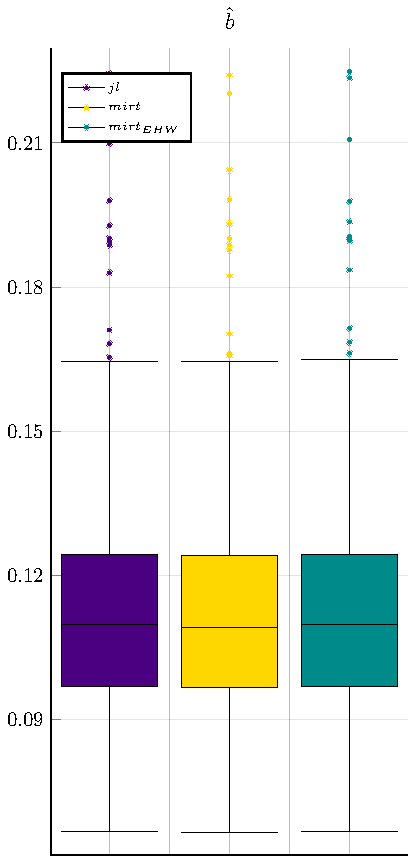
\includegraphics[width=.3\textwidth]{Figures/1a/RMSE_b.pdf} & 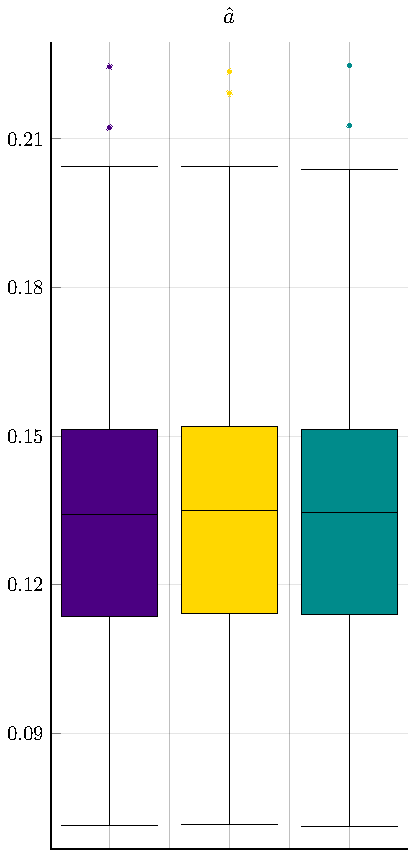
\includegraphics[width=.3\textwidth]{Figures/1a/RMSE_a.pdf} & 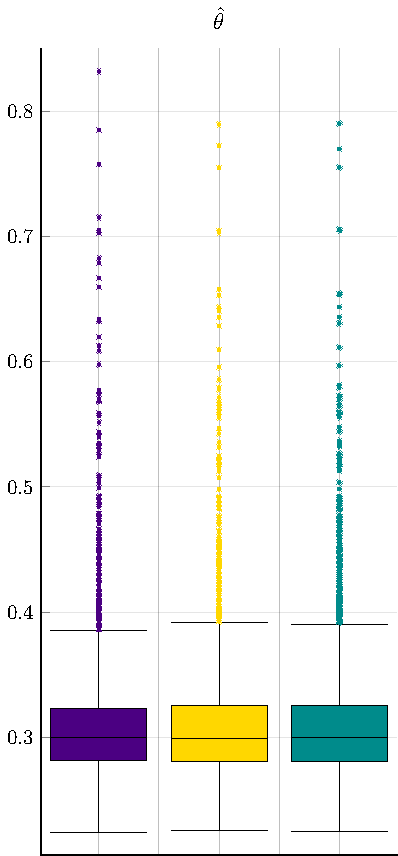
\includegraphics[width=.3\textwidth]{Figures/1a/RMSE_t.pdf}
	\end{tabular}
	\caption{Case 1a - Boxplots of RMSEs.}
	\label{fig:bpRMSE1a}
\end{figure}
\begin{figure}[ht]
	\centering \begin{tabular}[b]{c c c}
		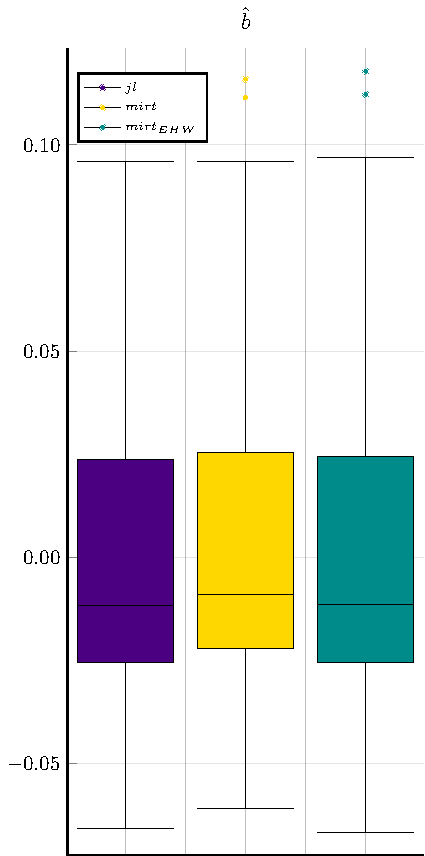
\includegraphics[width=.3\textwidth]{Figures/1a/BIAS_b.pdf} & 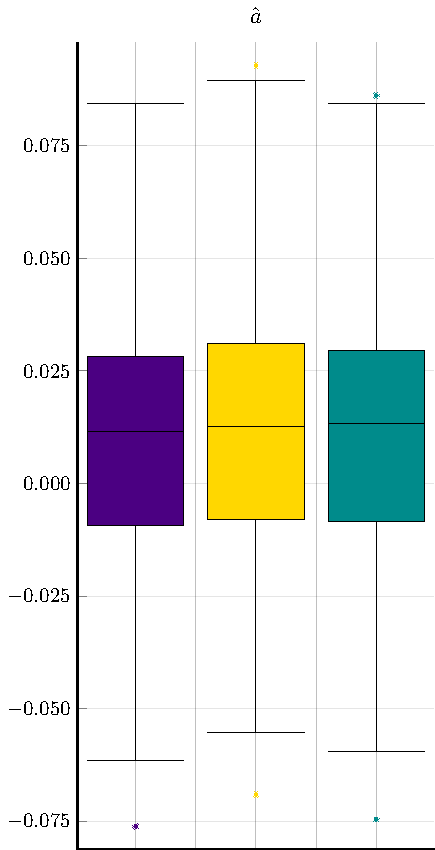
\includegraphics[width=.3\textwidth]{Figures/1a/BIAS_a.pdf} & 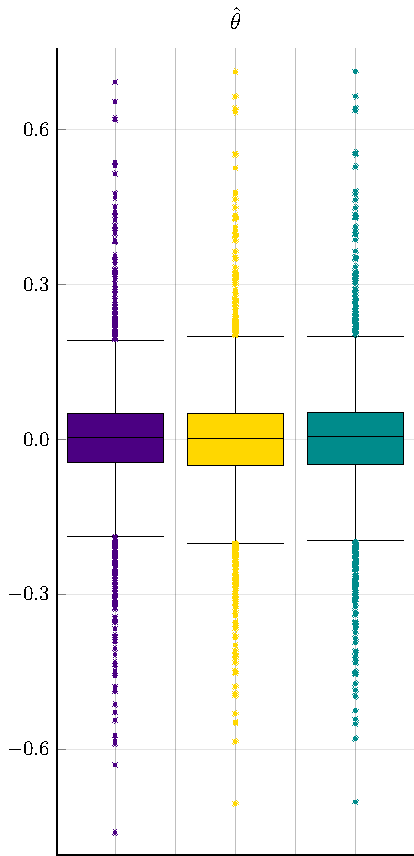
\includegraphics[width=.3\textwidth]{Figures/1a/BIAS_t.pdf}
	\end{tabular}
	\caption{Case 1a - Boxplots of BIASs.}
	\label{fig:bpBIAS1a}
\end{figure}
\begin{figure}[ht]
	\centering
	%\textbf{RMSEs of estimates with respect to the true values of item parameters and ability }\par\medskip
	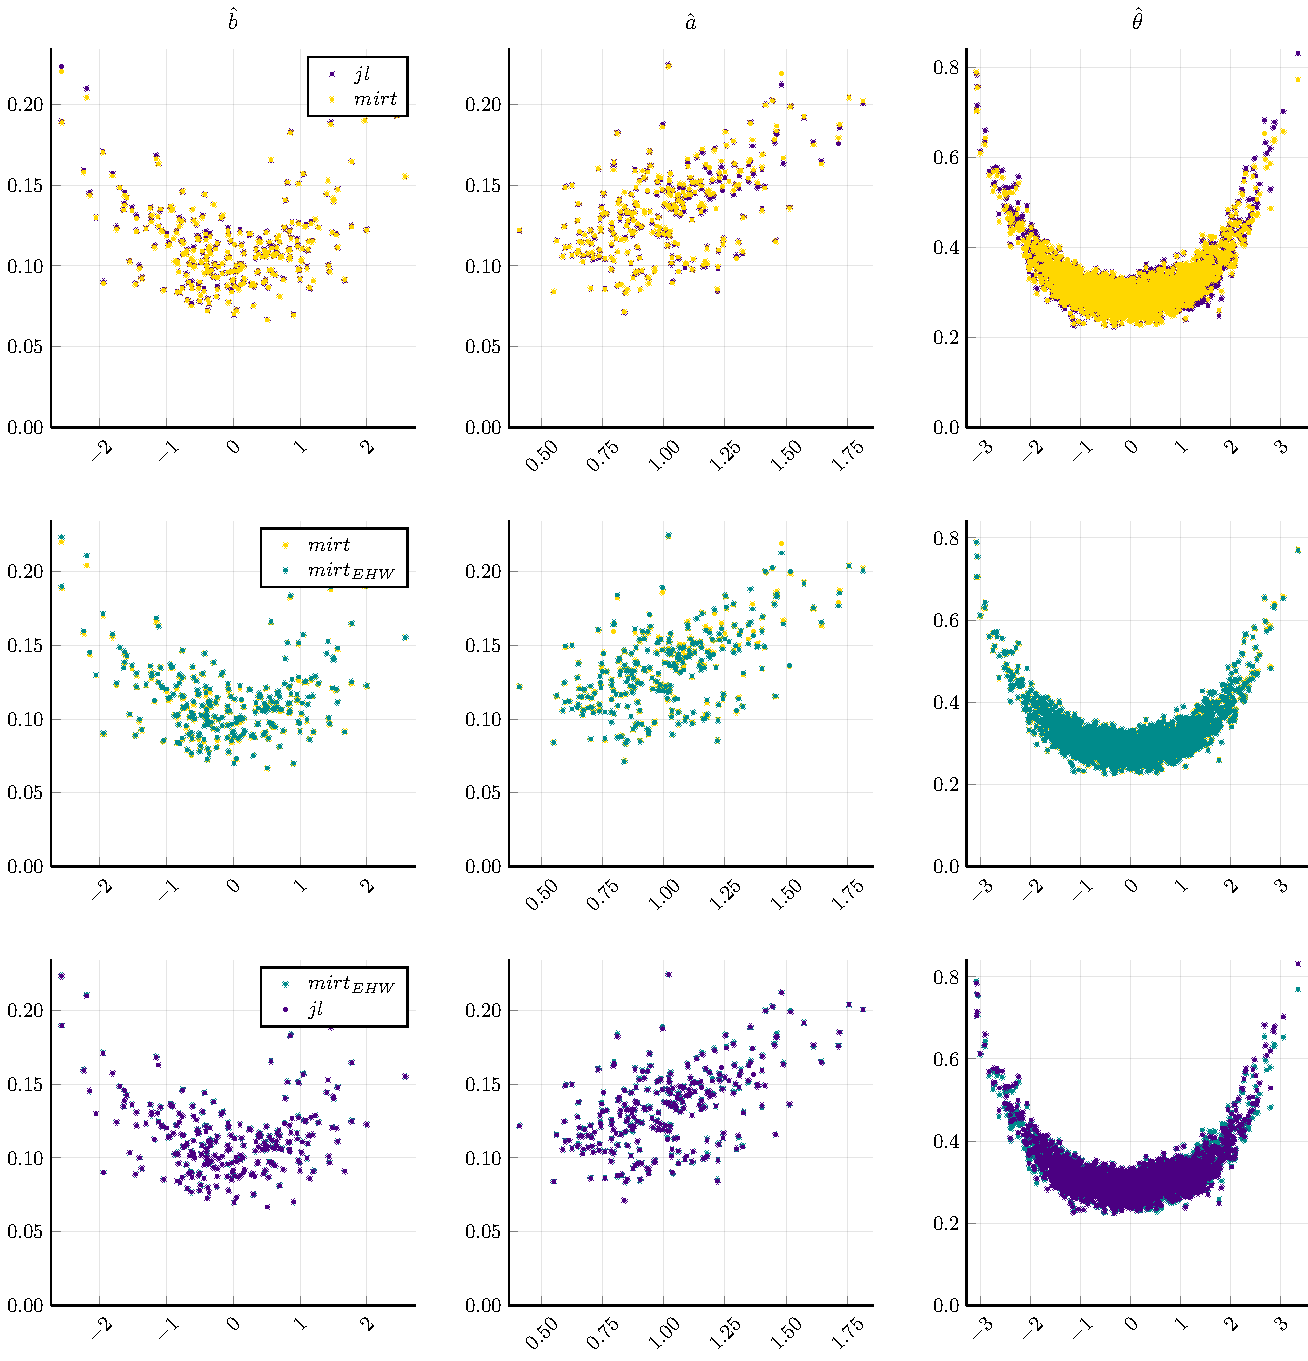
\includegraphics[width=\textwidth]{Figures/1a/RMSEscatter.pdf}
	\caption{Case 1b - Scatter plots of RMSEs.}
	\label{fig:spRMSE1a}
\end{figure}
\begin{figure}[ht]
	\centering
	%\textbf{BIASs of estimates with respect to the true values of item parameters and ability}\par\medskip
	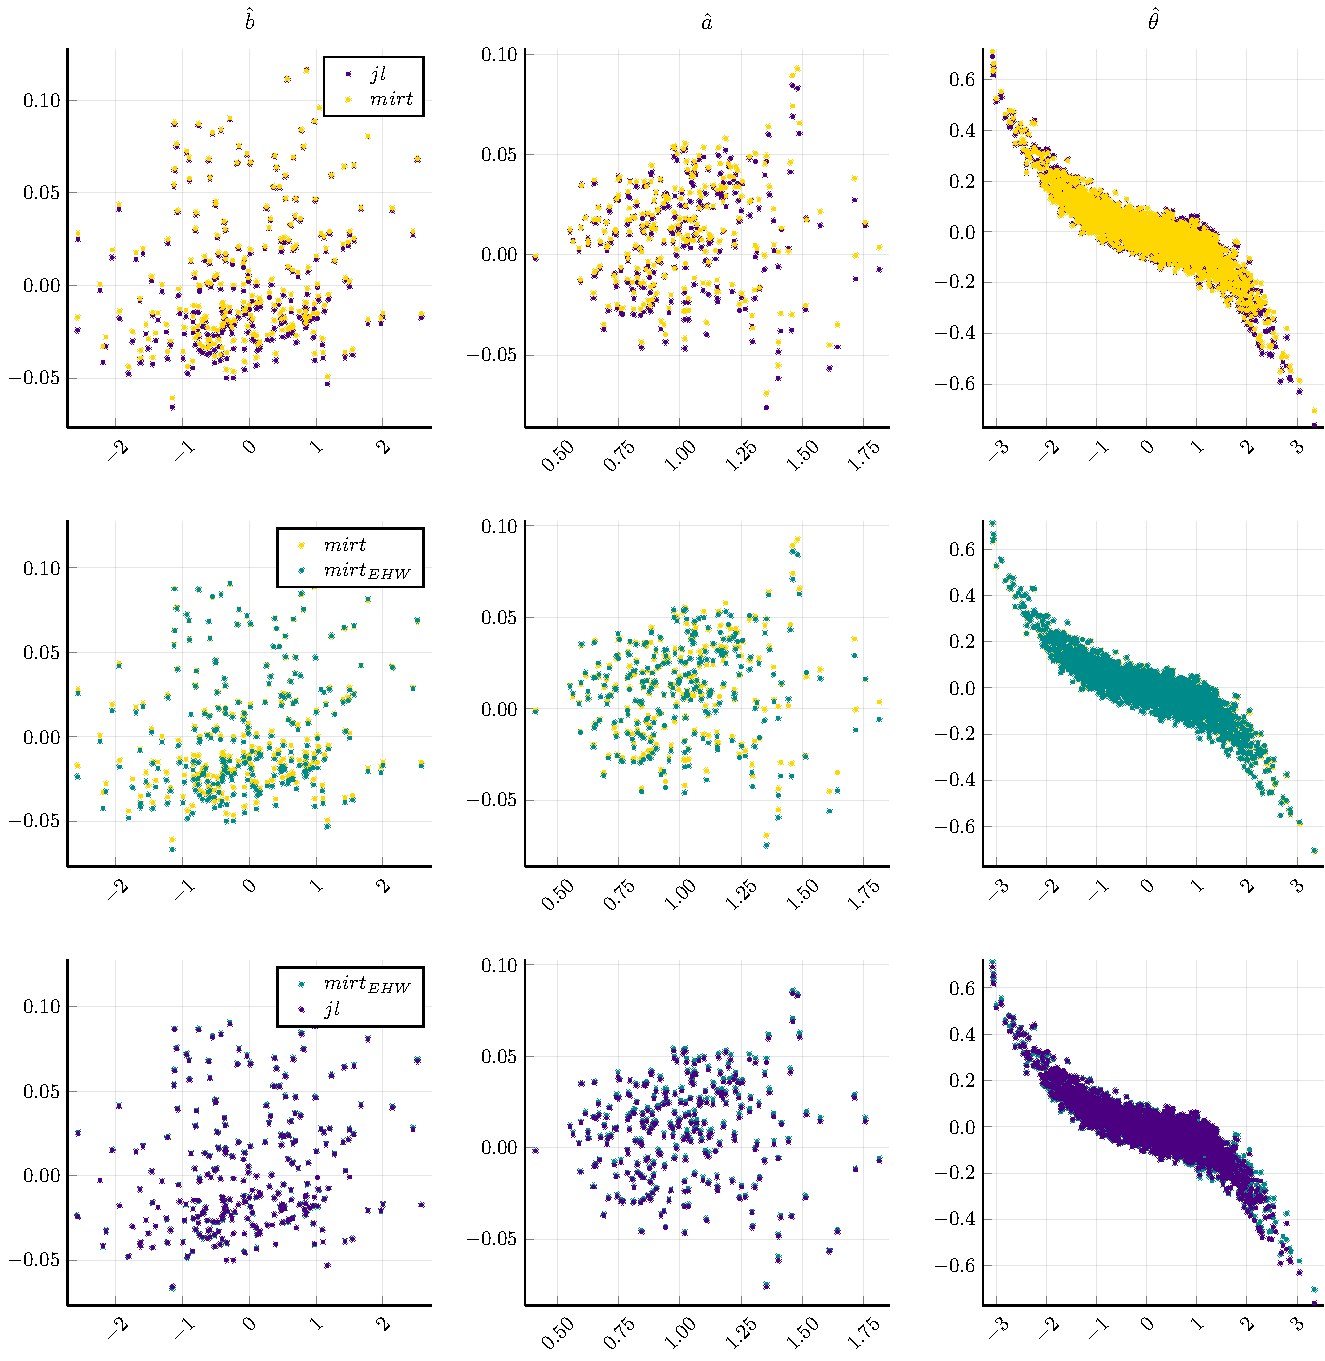
\includegraphics[width=\textwidth]{Figures/1a/BIASscatter.pdf}
	\caption{Case 1a - Scatter plots of BIASs }
	\label{fig:spBIAS1a}
\end{figure}
\subsection{Case 1b}
\begin{figure}[ht]
			\centering \begin{tabular}[b]{c c c}
		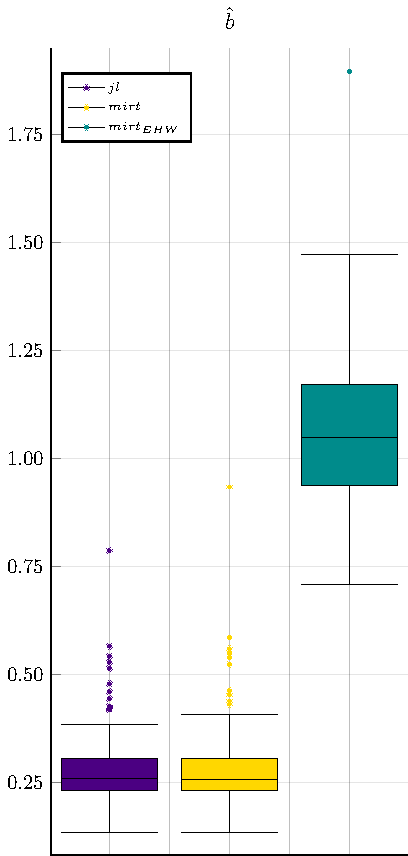
\includegraphics[width=.3\textwidth]{Figures/1b/RMSE_b.pdf} & 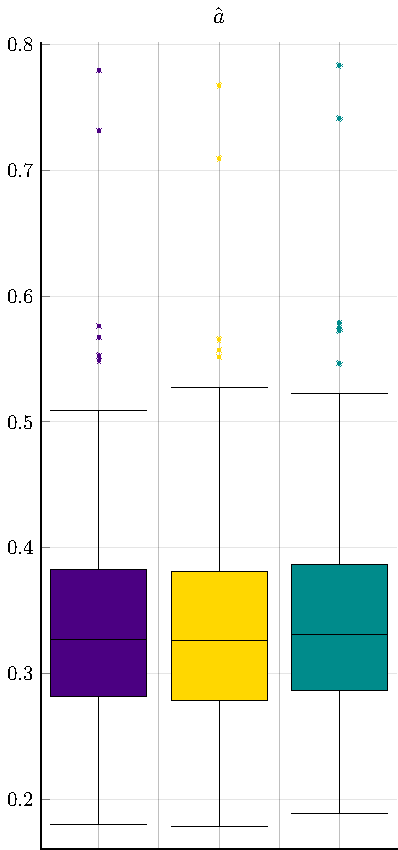
\includegraphics[width=.3\textwidth]{Figures/1b/RMSE_a.pdf} & 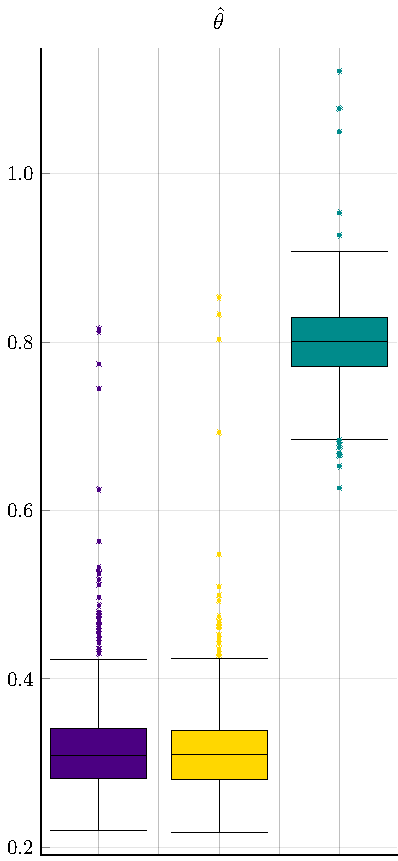
\includegraphics[width=.3\textwidth]{Figures/1b/RMSE_t.pdf}
	\end{tabular}
\caption{Case 1b - Boxplots of RMSEs.}
	\label{fig:bpRMSE1b}
\end{figure}
\begin{figure}[ht]
	\centering \begin{tabular}[b]{c c c}
		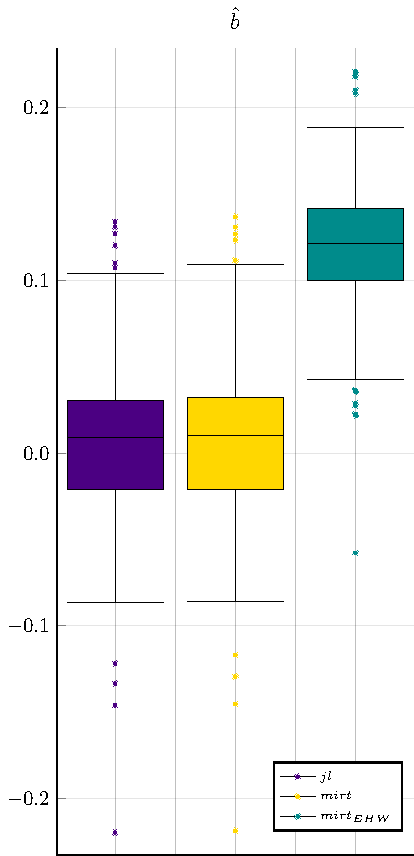
\includegraphics[width=.3\textwidth]{Figures/1b/BIAS_b.pdf} & 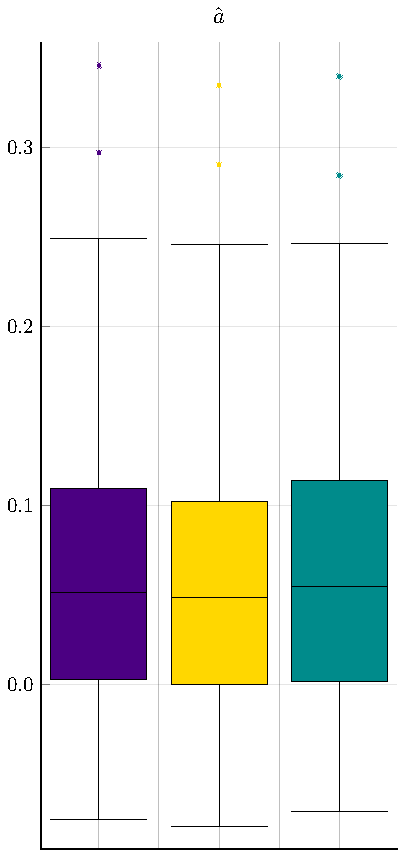
\includegraphics[width=.3\textwidth]{Figures/1b/BIAS_a.pdf} & 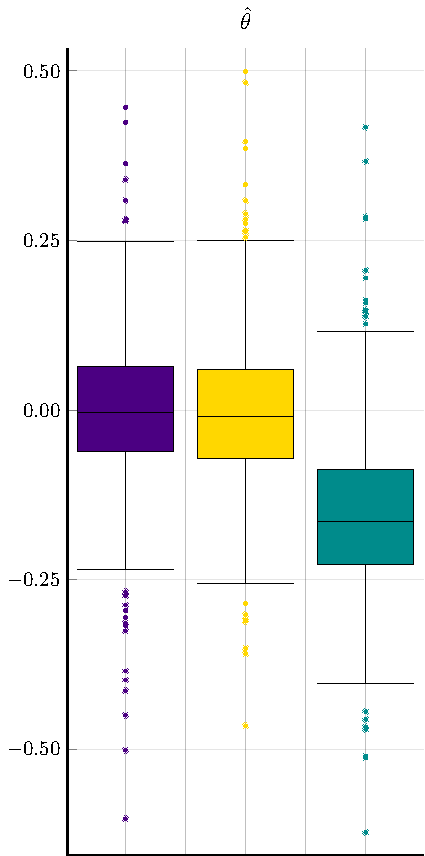
\includegraphics[width=.3\textwidth]{Figures/1b/BIAS_t.pdf}
	\end{tabular}
\caption{Case 1b - Boxplots of BIASs.}
	\label{fig:bpBIAS1b}
\end{figure}
\begin{figure}[ht]
	\centering
	%\textbf{RMSEs of estimates with respect to the true values of item parameters and ability }\par\medskip
	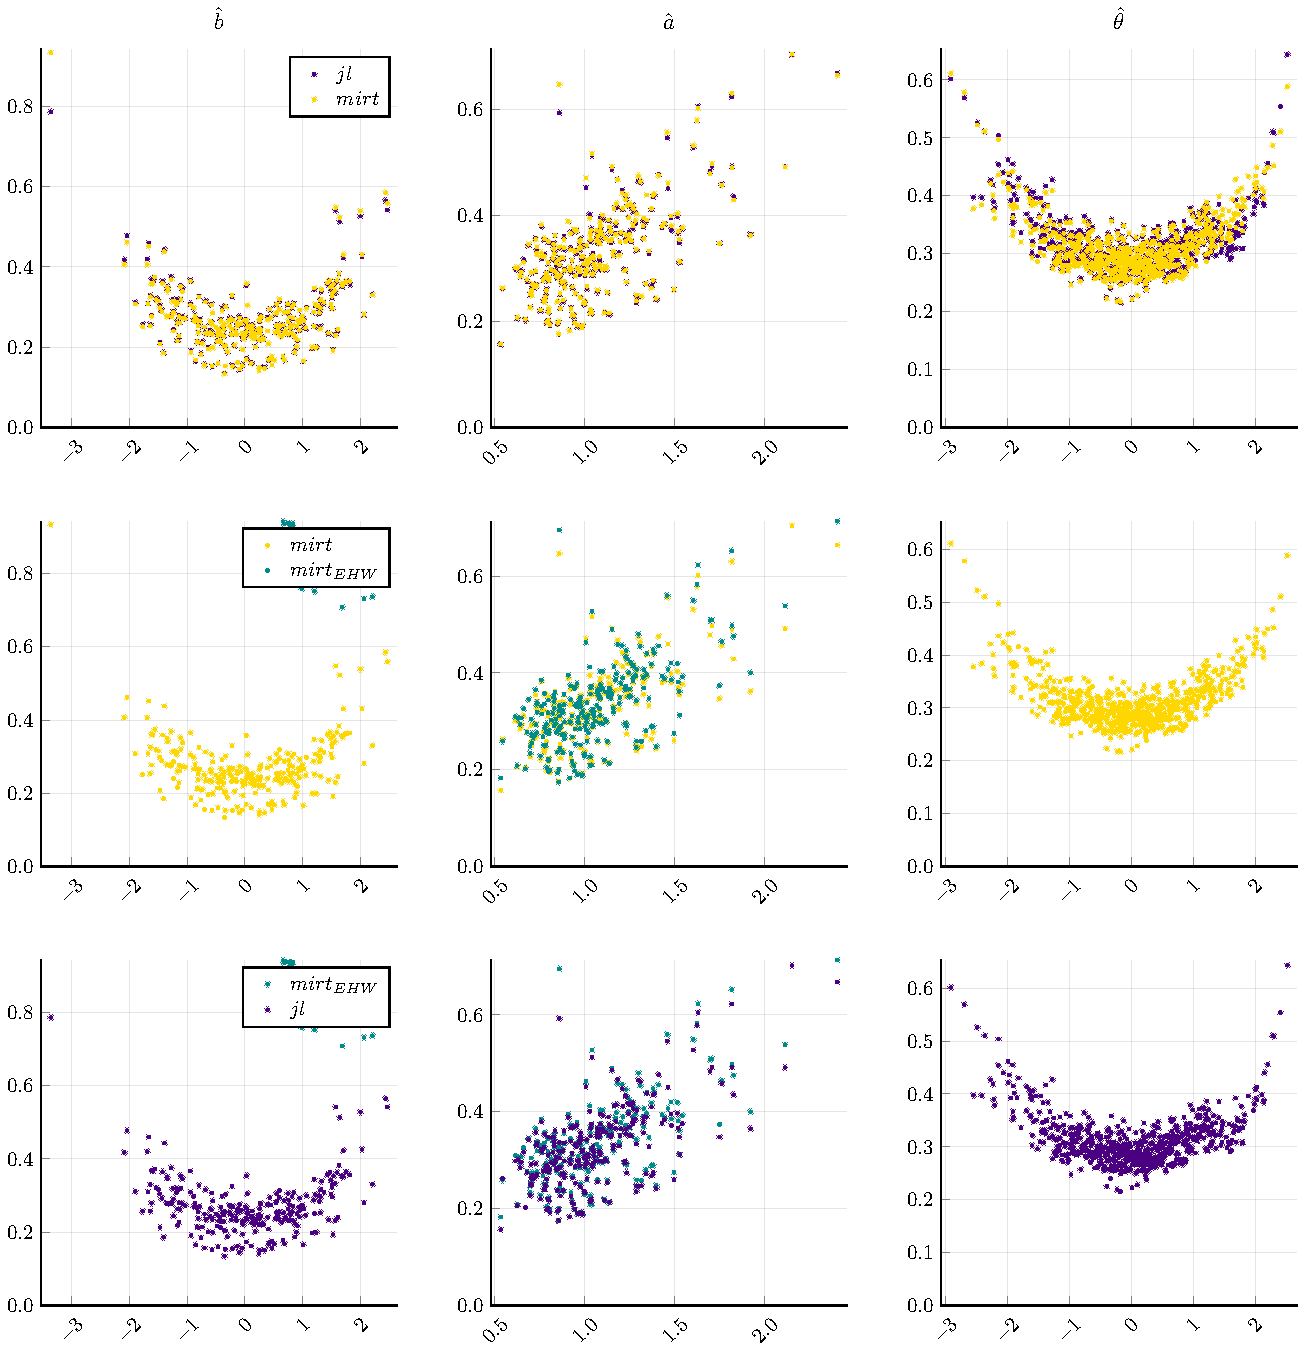
\includegraphics[width=\textwidth]{Figures/1b/RMSEscatter.pdf}
	\caption{Case 1b - Scatter plots of RMSEs.}
	\label{fig:spRMSE1b}
\end{figure}
\begin{figure}[ht]
	\centering
	%\textbf{BIASs of estimates with respect to the true values of item parameters and ability}\par\medskip
	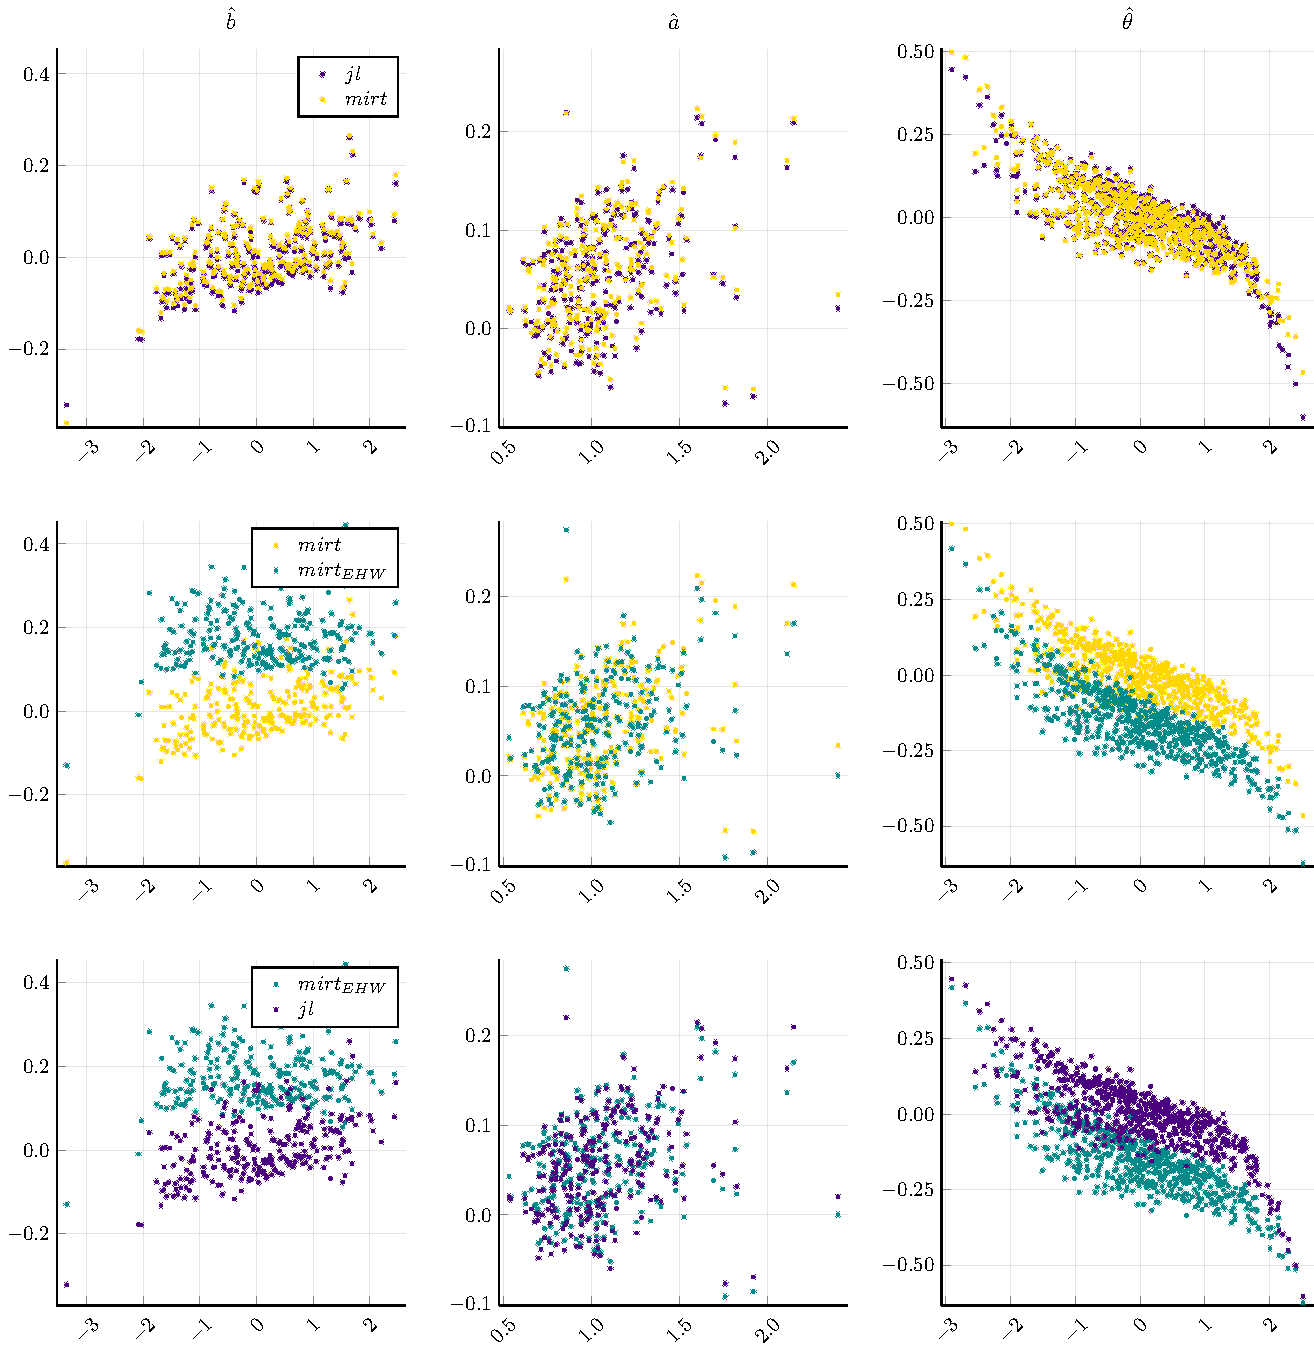
\includegraphics[width=\textwidth]{Figures/1b/BIASscatter.pdf}
	\caption{Case 1b - Scatter plots of BIASs }
	\label{fig:spBIAS1b}
\end{figure}
\subsection{Case 1c}
\begin{figure}[ht]
		\centering
		\begin{tabular}[b]{c c c}
		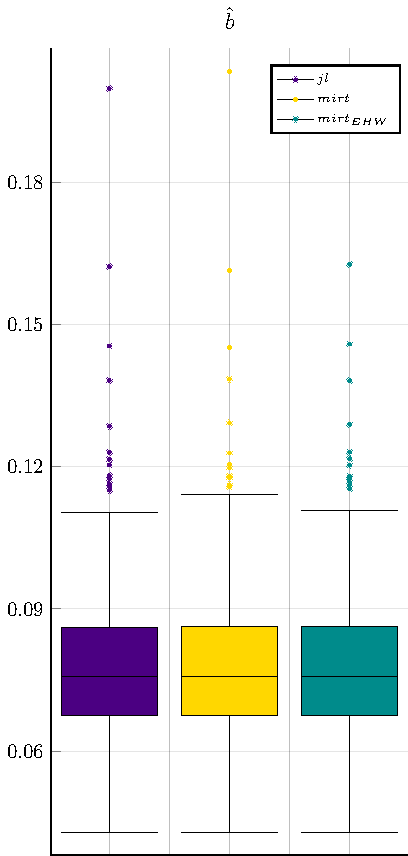
\includegraphics[width=.3\textwidth]{Figures/1c/RMSE_b.pdf} & 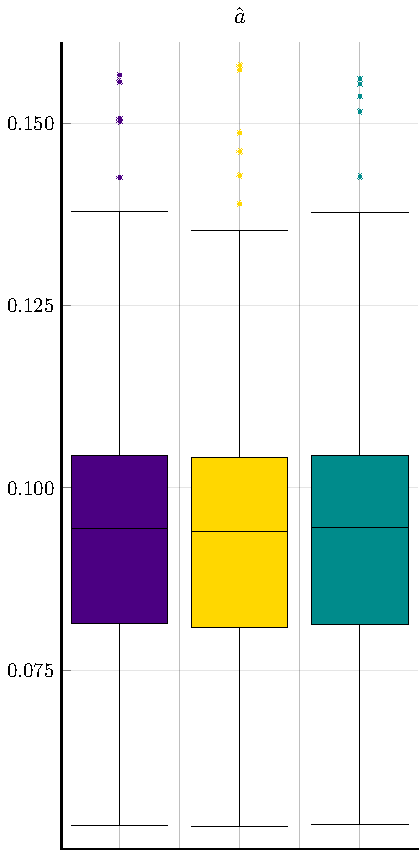
\includegraphics[width=.3\textwidth]{Figures/1c/RMSE_a.pdf} & 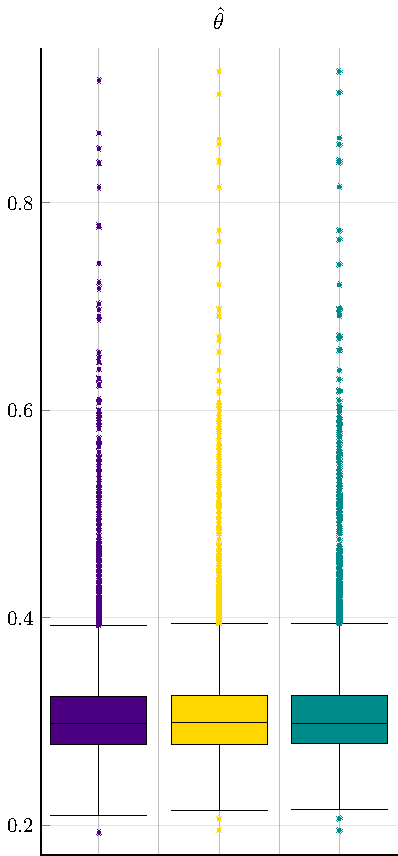
\includegraphics[width=.3\textwidth]{Figures/1c/RMSE_t.pdf}
	\end{tabular}
\caption{Case 1c - Boxplots of RMSEs.}
	\label{fig:bpRMSE1c}
\end{figure}
\begin{figure}[ht]
	
	\centering
	\begin{tabular}[b]{c c c}
		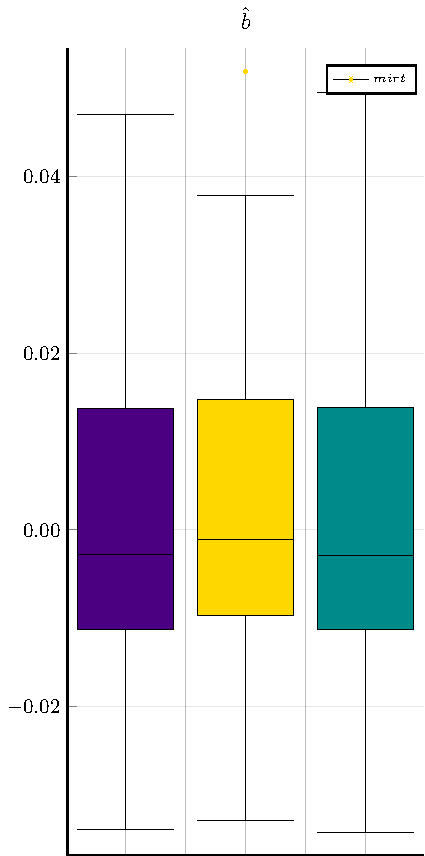
\includegraphics[width=.3\textwidth]{Figures/1c/BIAS_b.pdf} & 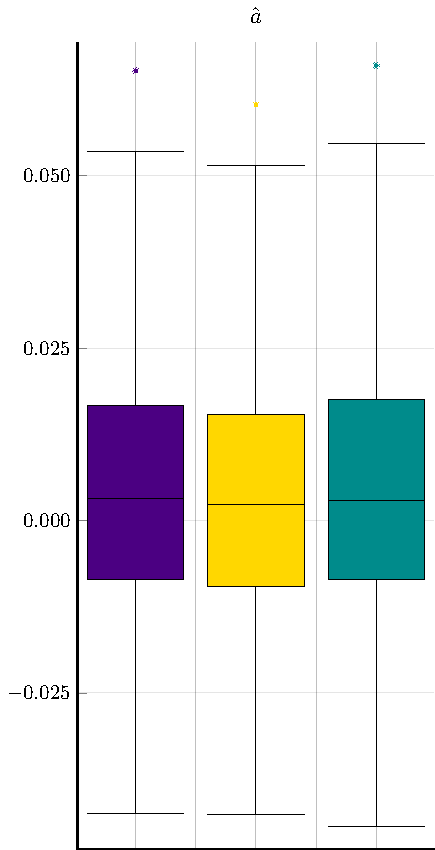
\includegraphics[width=.3\textwidth]{Figures/1c/BIAS_a.pdf} & 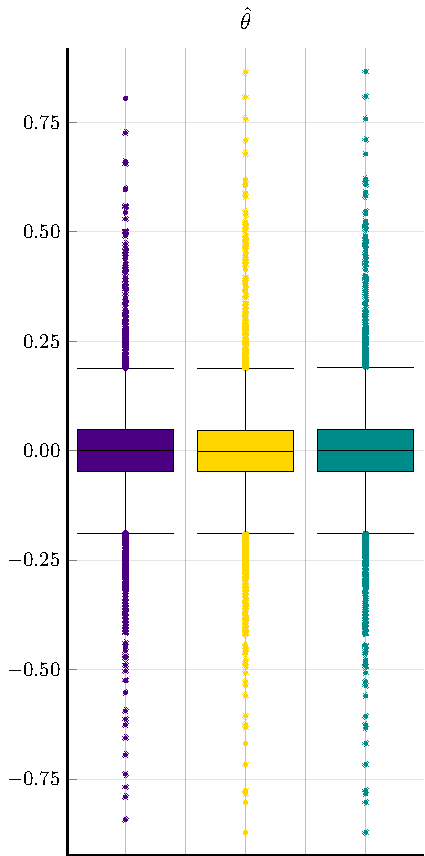
\includegraphics[width=.3\textwidth]{Figures/1c/BIAS_t.pdf}
	\end{tabular}
	\caption{Case 1c - Boxplots of BIASs.}
	\label{fig:bpBIAS1c}
\end{figure}
\begin{figure}[ht]
	\centering
	%\textbf{RMSEs of estimates with respect to the true values of item parameters and ability }\par\medskip
	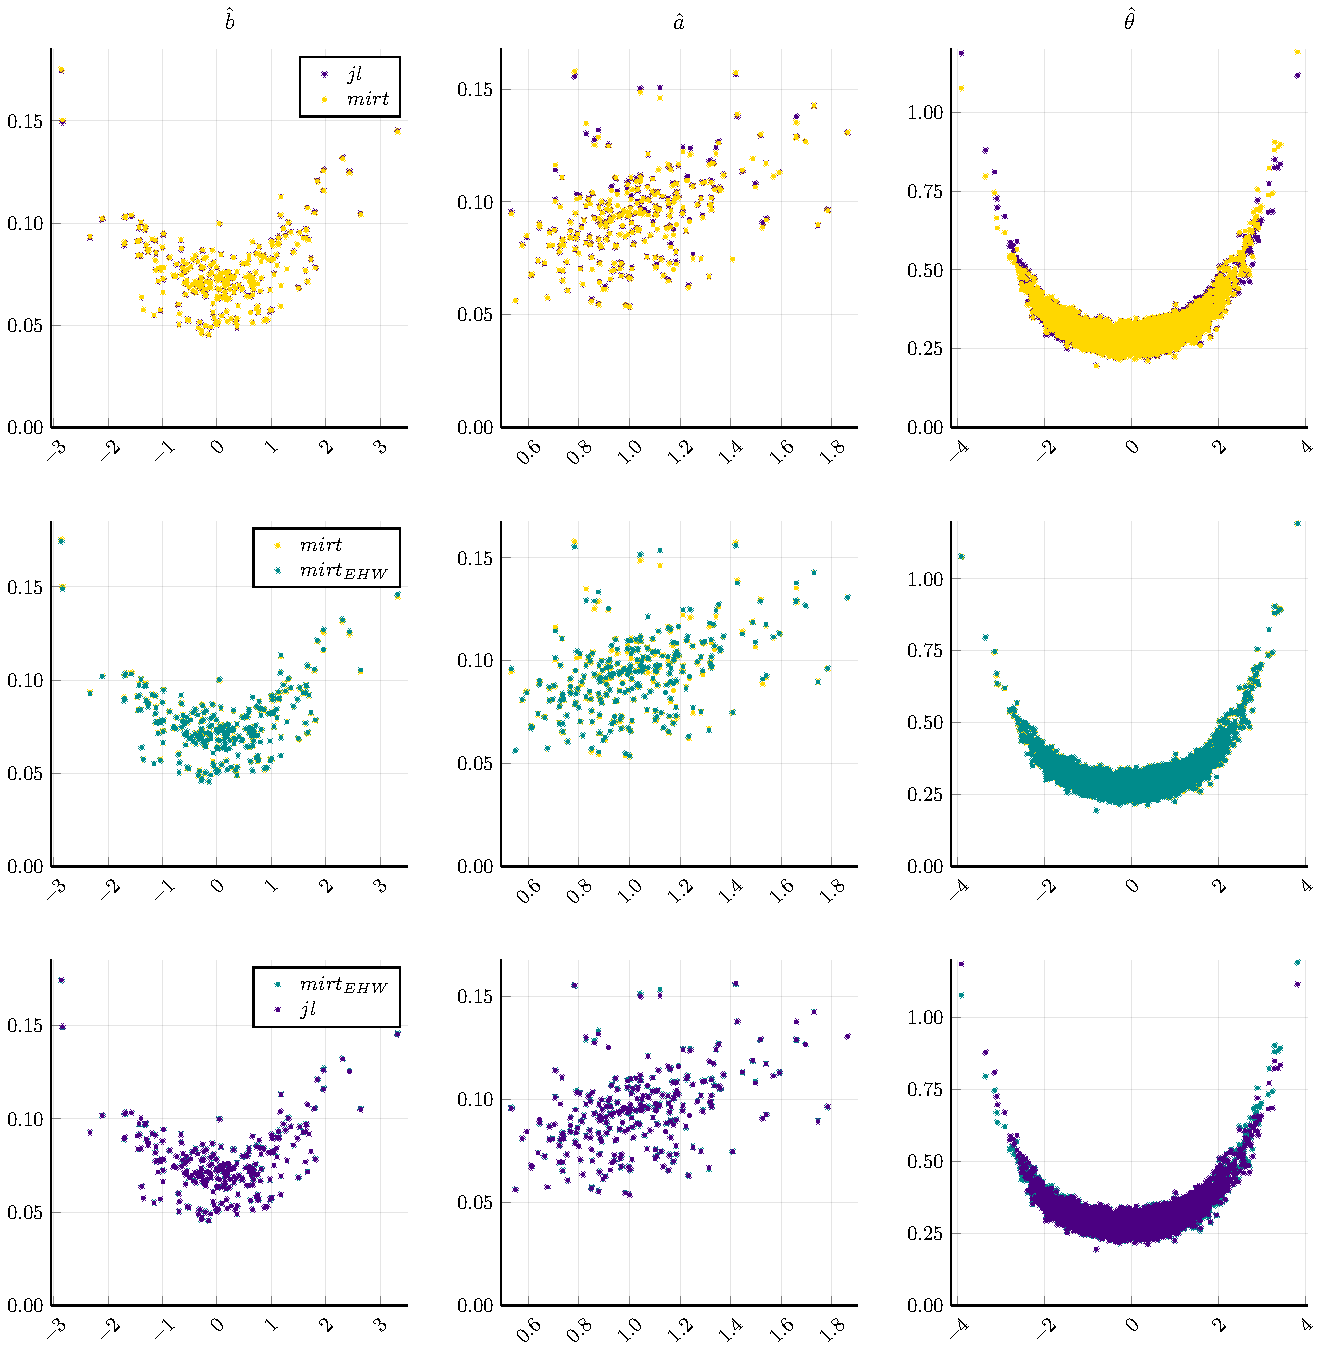
\includegraphics[width=\textwidth]{Figures/1c/RMSEscatter.pdf}
	\caption{Case 1c - Scatter plots of RMSEs.}
	\label{fig:spRMSE1c}
\end{figure}
\begin{figure}[ht]
	\centering
	%\textbf{BIASs of estimates with respect to the true values of item parameters and ability}\par\medskip
	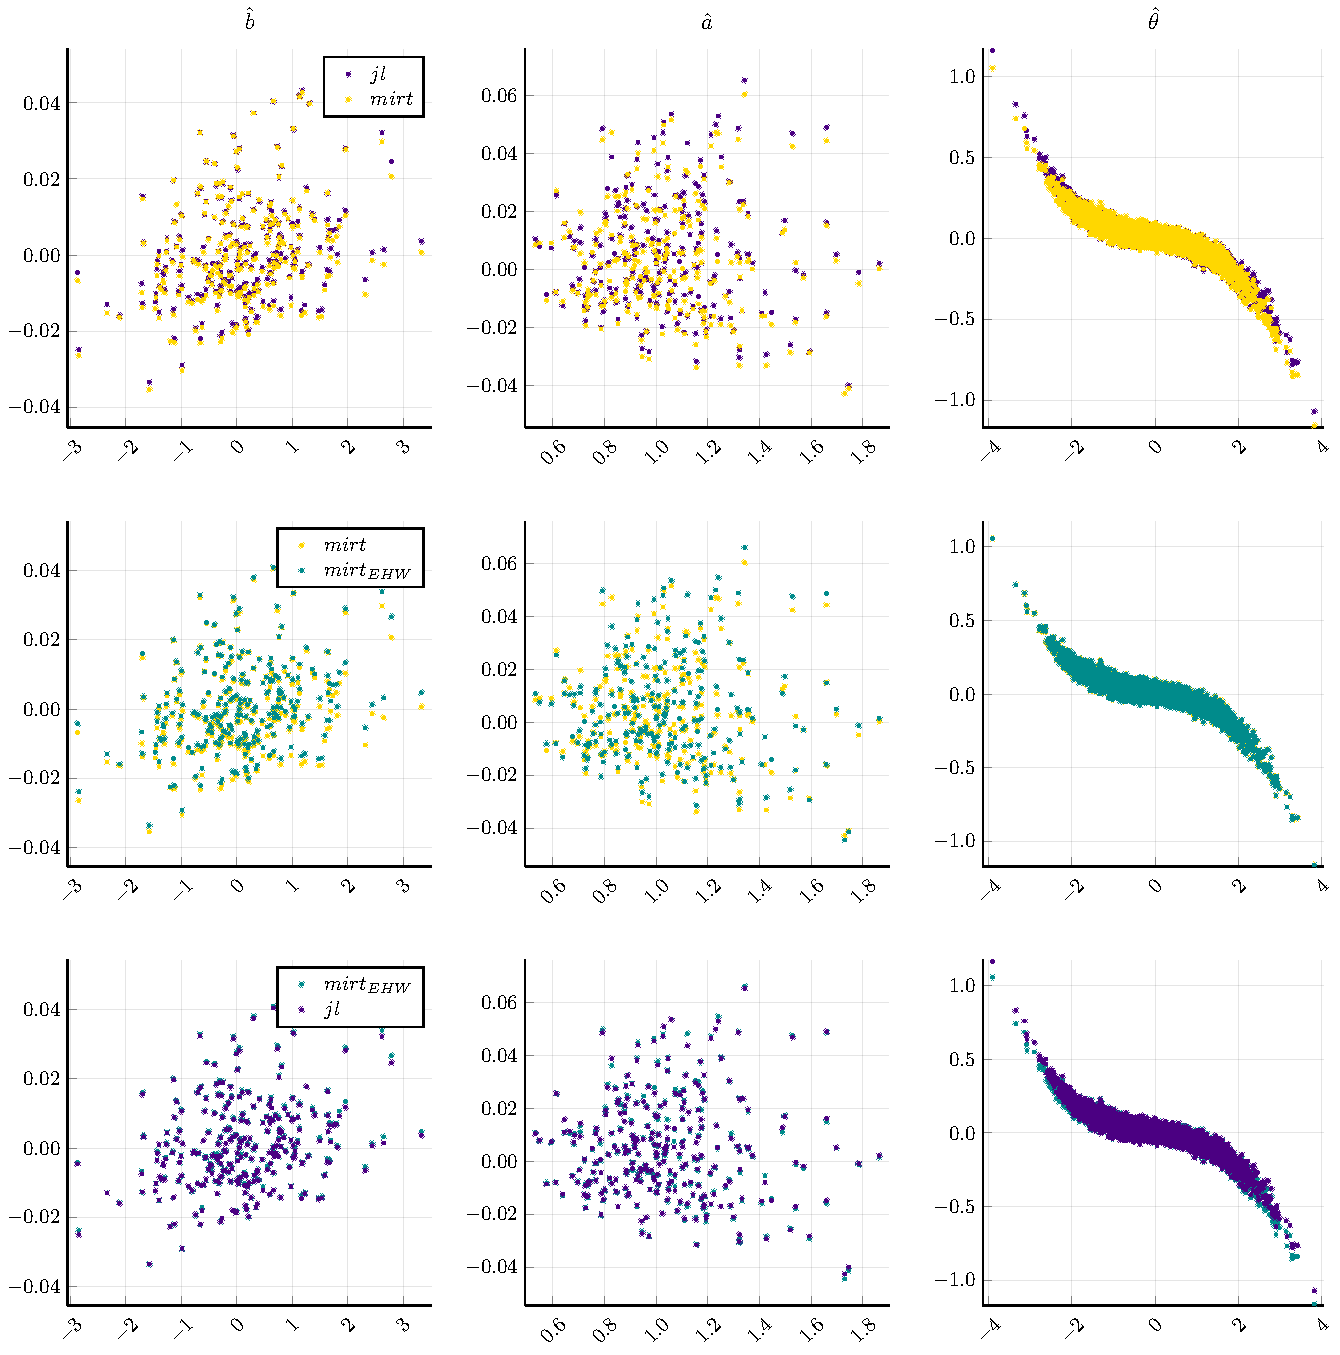
\includegraphics[width=\textwidth]{Figures/1c/BIASscatter.pdf}
	\caption{Case 1c - Scatter plots of BIASs }
	\label{fig:spBIAS1c}
\end{figure}
\subsection{Case 2a}
\begin{figure}[ht]
\centering
	 \begin{tabular}[b]{c c c}
		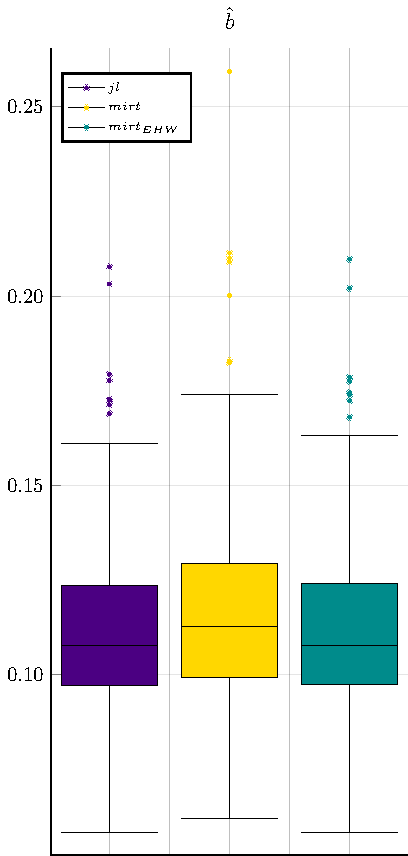
\includegraphics[width=.3\textwidth]{Figures/2a/RMSE_b.pdf} & 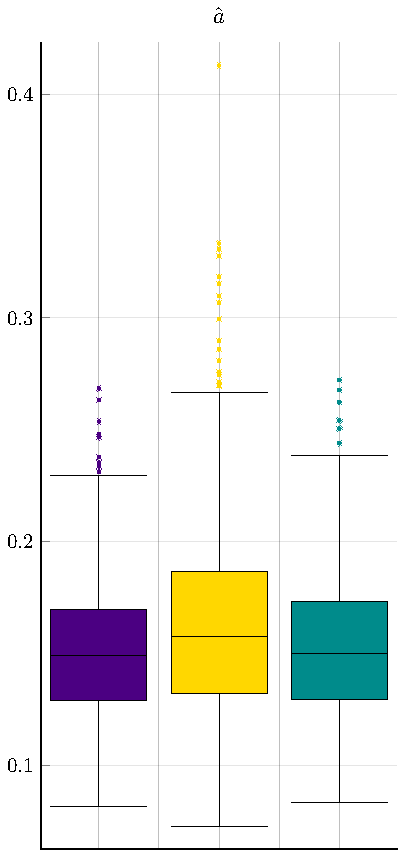
\includegraphics[width=.3\textwidth]{Figures/2a/RMSE_a.pdf} & 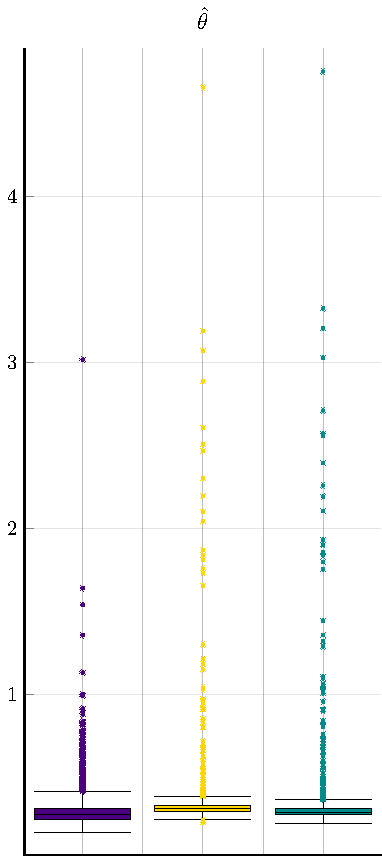
\includegraphics[width=.3\textwidth]{Figures/2a/RMSE_t.pdf}
	\end{tabular}
\caption{Case 2a - Boxplots of RMSEs.}
	\label{fig:bpRMSE2a}
\end{figure}
\begin{figure}[ht]
	\centering
	\begin{tabular}[b]{c c c}
		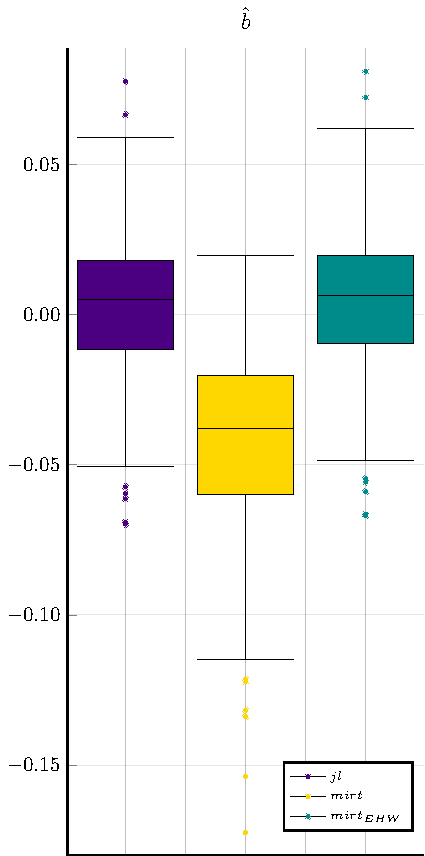
\includegraphics[width=.3\textwidth]{Figures/2a/BIAS_b.pdf} & 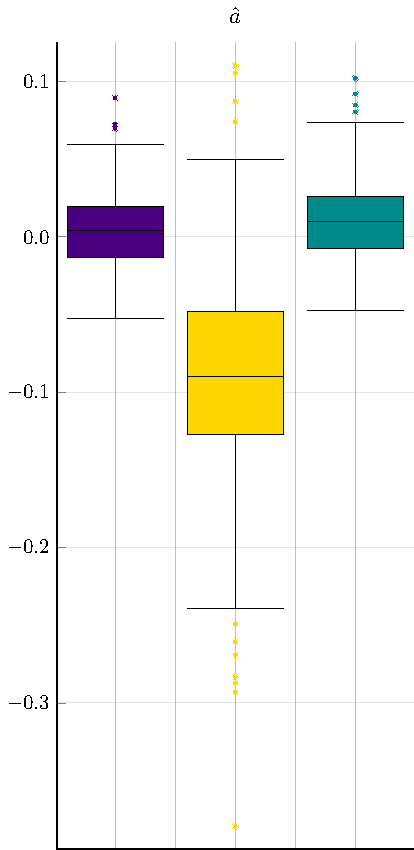
\includegraphics[width=.3\textwidth]{Figures/2a/BIAS_a.pdf} & 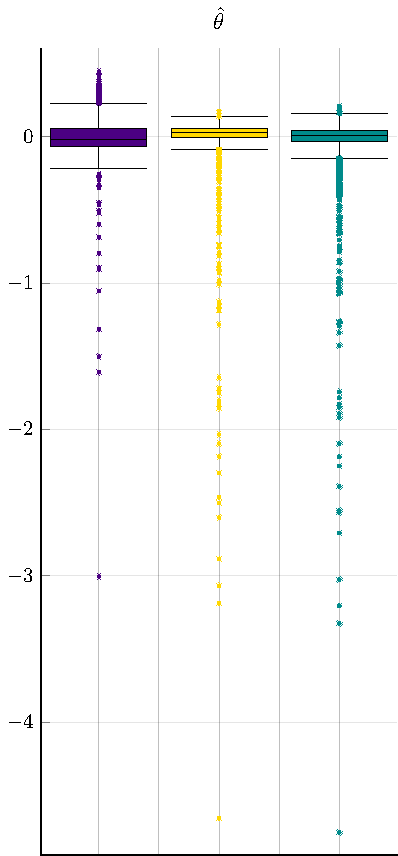
\includegraphics[width=.3\textwidth]{Figures/2a/BIAS_t.pdf}
	\end{tabular}
	\caption{Case 2a - Boxplots of BIASs.}
	\label{fig:bpBIAS2a}
\end{figure}
\begin{figure}[ht]
	\centering
	%\textbf{RMSEs of estimates with respect to the true values of item parameters and ability }\par\medskip
	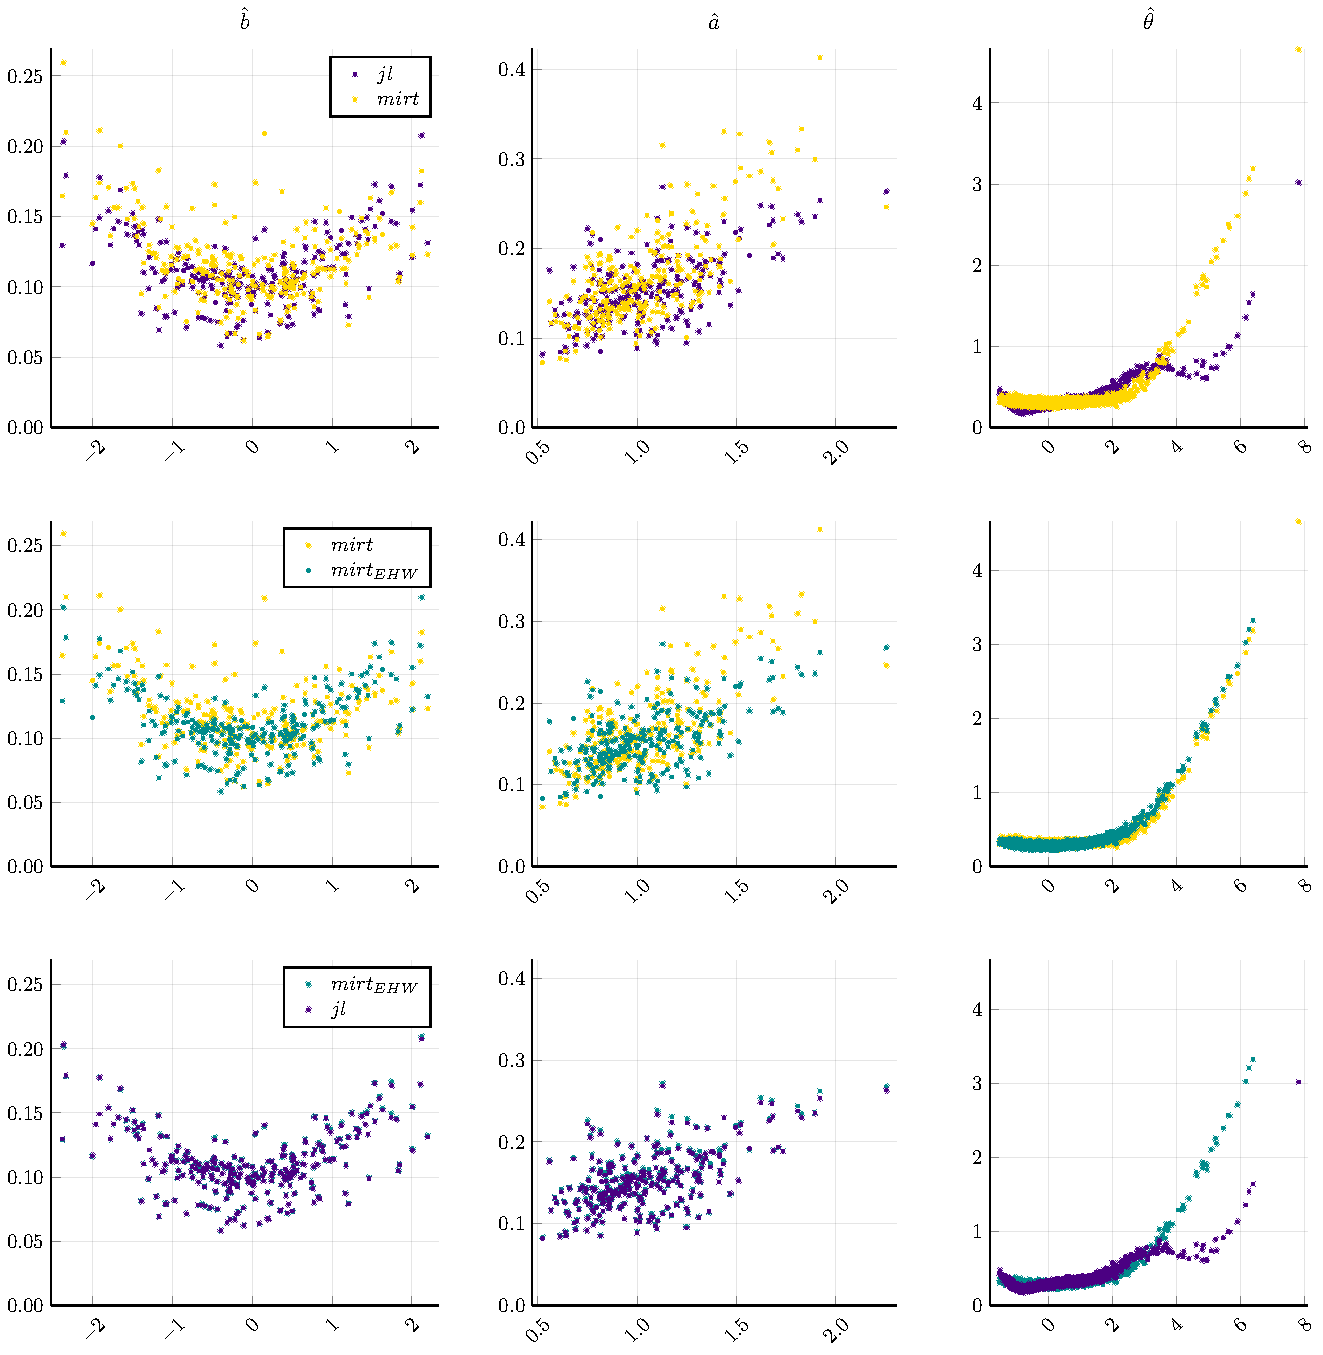
\includegraphics[width=\textwidth]{Figures/2a/RMSEscatter.pdf}
	\caption{Case 2a - Scatter plots of RMSEs.}
	\label{fig:spRMSE2a}
\end{figure}
\begin{figure}[ht]
	\centering
	%\textbf{BIASs of estimates with respect to the true values of item parameters and ability}\par\medskip
	\includegraphics[width=\textwidth]{Figures/2a/BIASscatter.pdf}
	\caption{Case 2a - Scatter plots of BIASs }
	\label{fig:spBIAS2a}
\end{figure}
\subsection{Case 2b}
\begin{figure}[ht]
	
	\centering
	\begin{tabular}[b]{c c c}
		\includegraphics[width=.3\textwidth]{Figures/2b/RMSE_b.pdf} & \includegraphics[width=.3\textwidth]{Figures/2b/RMSE_a.pdf} & \includegraphics[width=.3\textwidth]{Figures/2b/RMSE_t.pdf}
	\end{tabular}
\caption{Case 2b - Boxplots of RMSEs.}
	\label{fig:bpRMSE2b}
\end{figure}
\begin{figure}[ht]
	
	\centering \begin{tabular}[b]{c c c}
		\includegraphics[width=.3\textwidth]{Figures/2b/BIAS_b.pdf} & \includegraphics[width=.3\textwidth]{Figures/2b/BIAS_a.pdf} & \includegraphics[width=.3\textwidth]{Figures/2b/BIAS_t.pdf}
	\end{tabular}
	\caption{Case 2b - Boxplots of BIASs.}
	\label{fig:bpBIAS2b}
\end{figure}
\begin{figure}[ht]
	\centering
	%\textbf{RMSEs of estimates with respect to the true values of item parameters and ability }\par\medskip
	\includegraphics[width=\textwidth]{Figures/2b/RMSEscatter.pdf}
	\caption{Case 2b - Scatter plots of RMSEs.}
	\label{fig:spRMSE2b}
\end{figure}
\begin{figure}[ht]
	\centering
	%\textbf{BIASs of estimates with respect to the true values of item parameters and ability}\par\medskip
	\includegraphics[width=\textwidth]{Figures/2b/BIASscatter.pdf}
	\caption{Case 2b - Scatter plots of BIASs }
	\label{fig:spBIAS2b}
\end{figure}
\subsection{Case 3}
\begin{figure}[ht]
	
	\centering
	\begin{tabular}[b]{c c c}
		\includegraphics[width=.30\textwidth]{Figures/3/RMSE_b.pdf} & \includegraphics[width=.3\textwidth]{Figures/3/RMSE_a.pdf} & \includegraphics[width=.3\textwidth]{Figures/3/RMSE_t.pdf}
	\end{tabular}
\caption{Case 3 - Boxplots of RMSEs.}
	\label{fig:bpRMSE3}
\end{figure}
\begin{figure}[ht]
	
	\centering
	\begin{tabular}[b]{c c c}
		\includegraphics[width=.3\textwidth]{Figures/3/BIAS_b.pdf} & \includegraphics[width=.3\textwidth]{Figures/3/BIAS_a.pdf} & \includegraphics[width=.3\textwidth]{Figures/3/BIAS_t.pdf}
	\end{tabular}
	\caption{Case 3 - Boxplots of BIASs.}
	\label{fig:bpBIAS3}
\end{figure}
\begin{figure}[ht]
	\centering
	%\textbf{RMSEs of estimates with respect to the true values of item parameters and ability }\par\medskip
	\includegraphics[width=\textwidth]{Figures/3/RMSEscatter.pdf}
	\caption{Case 3 - Scatter plots of RMSEs.}
	\label{fig:spRMSE3}
\end{figure}
\begin{figure}[ht]
	\centering
	%\textbf{BIASs of estimates with respect to the true values of item parameters and ability}\par\medskip
	\includegraphics[width=\textwidth]{Figures/3/BIASscatter.pdf}
	\caption{Case 3 - Scatter plots of BIASs }
	\label{fig:spBIAS3}
\end{figure}
\subsection{Case 4}
\begin{figure}[ht]
	\centering
	\begin{tabular}[b]{c c c}
		\includegraphics[width=.3\textwidth]{Figures/4/RMSE_b.pdf} & \includegraphics[width=.3\textwidth]{Figures/4/RMSE_a.pdf} & \includegraphics[width=.3\textwidth]{Figures/4/RMSE_t.pdf}
	\end{tabular}
\caption{Case 4 - Boxplots of RMSEs.}
	\label{fig:bpRMSE4}
\end{figure}
\begin{figure}[ht]
	
	\centering
	\begin{tabular}[b]{c c c}
		\includegraphics[width=.3\textwidth]{Figures/4/BIAS_b.pdf} & \includegraphics[width=.3\textwidth]{Figures/4/BIAS_a.pdf} & \includegraphics[width=.3\textwidth]{Figures/4/BIAS_t.pdf}
	\end{tabular}
	\caption{Case 4 - Boxplots of BIASs.}
	\label{fig:bpBIAS4}
\end{figure}
\begin{figure}[ht]
	\centering
	%\textbf{RMSEs of estimates with respect to the true values of item parameters and ability }\par\medskip
	\includegraphics[width=\textwidth]{Figures/4/RMSEscatter.pdf}
	\caption{Case 4 - Scatter plots of RMSEs.}
	\label{fig:spRMSE4}
\end{figure}
\begin{figure}[ht]
	\centering
	%\textbf{BIASs of estimates with respect to the true values of item parameters and ability}\par\medskip
	\includegraphics[width=\textwidth]{Figures/4/BIASscatter.pdf}
	\caption{Case 4 - Scatter plots of BIASs }
	\label{fig:spBIAS4}
\end{figure}


	%\include{Appendices/Relazione}
	%\include{Appendices/AppendixB}
	%\include{Appendices/AppendixC}
	
	%----------------------------------------------------------------------------------------
	%	BIBLIOGRAPHY
	%----------------------------------------------------------------------------------------
	% with biblatex
	\printbibliography
	
	%----------------------------------------------------------------------------------------
	
\end{document}  
